\documentclass[a4paper]{article}
\usepackage{import}
\usepackage{graphicx}
\usepackage{float}
\usepackage{pgfplots}
\usepackage{listings}
\usepackage{enumitem}
\usepackage{textcomp}
\usepackage{tikz}
\usetikzlibrary{decorations.pathreplacing} % for angle arc
\usetikzlibrary{angles, quotes, calc, positioning, trees} % for drawing angles
\pgfplotsset{compat=1.18,width=10cm}
\usepackage{tikz-cd}
\usepackage{booktabs}
\usepackage{cancel}
\usepackage{amsmath}
\usepackage{minted}
\usepackage{csquotes}
\usepackage{gensymb}
\usepackage{forest}
\usepackage{amsthm}
\usepackage{amssymb}
\usepackage{fontawesome} 
\usepackage{varwidth}
\usepackage{pgfplots}
\usepackage{lipsum}
\usepackage{mdframed} 
\usepackage{color}   
\usepackage{hyperref}
\newmdtheoremenv{theo}{Theorem}
\usepackage{mathtools}
\DeclarePairedDelimiter\ceil{\lceil}{\rceil}
\DeclarePairedDelimiter\floor{\lfloor}{\rfloor}

\hypersetup{
    colorlinks=true, %set true if you want colored links
    linktoc=all,     %set to all if you want both sections and subsections linked
    linkcolor=black,  %choose some color if you want links to stand out
}

% Define theorem styles
\newtheorem{theorem}{Theorem}[section]    % Theorems numbered within sections
\newtheorem{lemma}[theorem]{Lemma}        % Lemmas use the same counter as theorems
\newtheorem{corollary}[theorem]{Corollary} % Corollaries use the same counter as theorems
\newtheorem{proposition}[theorem]{Proposition} % Proposition uses the same counter
\newtheorem{property}[theorem]{Property}
\theoremstyle{definition}
\newtheorem{definition}[theorem]{Definition} % Now uses the same counter as theorems


% Remark-style theorem
\theoremstyle{remark}
\newtheorem{remark}[theorem]{Remark}

% Boxed environment for theorems
\newmdenv[
  linewidth=0.8pt,
  roundcorner=5pt,
  linecolor=black,
  backgroundcolor=white!5,
  skipabove=\baselineskip,
  skipbelow=\baselineskip,
  innerleftmargin=10pt,
  innerrightmargin=10pt,
  innertopmargin=5pt,
  innerbottommargin=5pt
]{thmbox}

% Custom proof environment (also boxed)
\renewenvironment{proof}[1][Proof]{%
  \begin{mdframed}[linewidth=0.8pt, roundcorner=5pt, linecolor=black, skipabove=\baselineskip, skipbelow=\baselineskip, innertopmargin=5pt, innerbottommargin=5pt]%
  \noindent\textbf{#1. }%
}{%
  \end{mdframed}%
}

% Redefine theorem environments to use thmbox
\let\oldtheorem\theorem
\renewenvironment{theorem}{\begin{thmbox}\begin{oldtheorem}}{\end{oldtheorem}\end{thmbox}}

\let\oldlemma\lemma
\renewenvironment{lemma}{\begin{thmbox}\begin{oldlemma}}{\end{oldlemma}\end{thmbox}}

\let\oldcorollary\corollary
\renewenvironment{corollary}{\begin{thmbox}\begin{oldcorollary}}{\end{oldcorollary}\end{thmbox}}

\let\oldproposition\proposition
\renewenvironment{proposition}{\begin{thmbox}\begin{oldproposition}}{\end{oldproposition}\end{thmbox}}

\let\oldproperty\property
  \renewenvironment{property}{\begin{oldproperty}}{\end{oldproperty}}


% Reference shortcuts
\newcommand{\thmref}[1]{Theorem~\ref{#1}}
\newcommand{\lemref}[1]{Lemma~\ref{#1}}
\newcommand{\corref}[1]{Corollary~\ref{#1}}
\newcommand{\propref}[1]{Property~\ref{#1}} 

% To customize QED symbol
\renewcommand{\qedsymbol}{$\blacksquare$}

\usetikzlibrary{decorations.pathreplacing} % for angle arc
\usetikzlibrary{angles, quotes, calc} % for drawing angles

\usepackage{color}   %May be necessary if you want to color links
\usepackage{hyperref}
\hypersetup{
    colorlinks=true, %set true if you want colored links
    linktoc=all,     %set to all if you want both sections and subsections linked
    linkcolor=black,  %choose some color if you want links to stand out
}

\usepackage{xcolor}
\usepackage[most]{tcolorbox}


% Define a custom tcolorbox environment for examples
\newtcolorbox{examplebox}[2][]{
  colback=blue!5!white,
  colframe=blue!30!black,
  title=#2,
  boxrule=0mm,
  fonttitle=\bfseries,
  width=\textwidth,
  breakable,
  #1
}

\newtcolorbox{definizione}[2] {
  colback=green!5!white,
  colframe=green!30!black,
  title=#2,
  boxrule=0mm,
  fonttitle=\bfseries,
  width=\textwidth,
  breakable,
  #1
}

\definecolor{codegreen}{rgb}{0,0.6,0}
\definecolor{codegray}{rgb}{0.5,0.5,0.5}
\definecolor{codepurple}{rgb}{0.58,0,0.82}
\definecolor{backcolour}{rgb}{0.95,0.95,0.92}

\lstdefinestyle{mystyle}{
    backgroundcolor=\color{backcolour},   
    commentstyle=\color{codegreen},
    keywordstyle=\color{magenta},
    numberstyle=\tiny\color{codegray},
    stringstyle=\color{codepurple},
    basicstyle=\ttfamily\footnotesize,
    breakatwhitespace=false,         
    breaklines=true,                 
    captionpos=b,                    
    keepspaces=true,                 
    numbers=left,                    
    numbersep=5pt,                  
    showspaces=false,                
    showstringspaces=false,
    showtabs=false,                  
    tabsize=2
}

\lstset{style=mystyle}

\makeatletter
\renewcommand*\env@matrix[1][*\c@MaxMatrixCols c]{%
  \hskip -\arraycolsep
  \let\@ifnextchar\new@ifnextchar
  \array{#1}}
\makeatother

\title{Sistemi}
\author{Università di Verona\\Imbriani Paolo -VR500437\\Professor Francesco Visentin}

\begin{document}

\begin{figure}
    \centering
    
\includegraphics[width=0.3\textwidth]{UniversityofVerona.png}
    \label{fig:centered-image}
\end{figure}

\maketitle 

\pagebreak

\tableofcontents

\pagebreak

\section{Trasformata di Laplace}

\begin{definition}
$v(t)$ è definito nel tempo. V(s) è la sua trasformata. 
    \[\mathcal{L}[f(t)](s) = \int_{0}^{+\infty} v(t)e^{-st}dt\]
\end{definition}

\begin{figure}[H]
    \centering
    \caption{$\alpha \ge max\{\lambda_i\}$}
    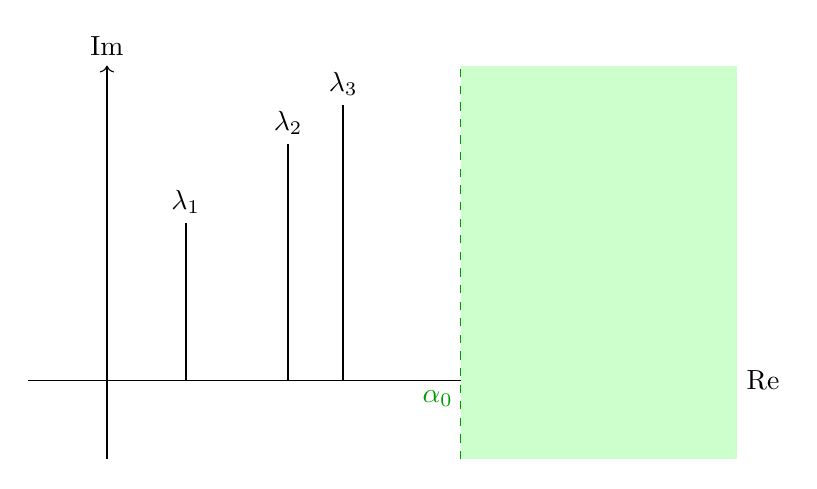
\begin{tikzpicture}
        % Axes
        \draw[->] (-1, 0) -- (8, 0) node[right] {$\operatorname{Re}$};
        \draw[->] (0, -1) -- (0, 4) node[above] {$\operatorname{Im}$};
    

        \draw[thick] (1, 0) -- (1, 2);
        \node[above] at (1, 2) {$\lambda_1$};
        \draw[thick] (2.3, 0) -- (2.3, 3);
        \node[above] at (2.3, 3) {$\lambda_2$};
        \draw[thick] (3, 0) -- (3, 3.5);
        \node[above] at (3, 3.5) {$\lambda_3$};
    
        % Dashed line for region boundary at x = 4.5
        \draw[dashed, thick, green!60!black] (4.5, -1) -- (4.5, 4);
        \node[below, green!60!black] at (4.2, 0) {$\alpha_0$};
    
        % Green filled region of convergence
        \fill[green!20] (4.5, -1) rectangle (8, 4);

    \end{tikzpicture}
\end{figure}


\subsection{Proprietà}

La trasformata di LaPlace ha svariate utili proprietà che possiamo utilizzare a nostro vantaggio:
\indent
\begin{property}
\label{prop:linearity_lap}
    \textbf{Linearità}: \[a_1v_1(t) + a_2v_2(t) = a_1V_1(s) + a_2V_2(s)\]
\end{property}
\begin{property}
\label{prop:traslas_time_lap}
    \textbf{Traslazione nel dom. del tempo: } \[\mathcal{L}[v(t-\tau)](s) = \overbrace{e^{-st}V(s)}^{\tau > 0}\]
\end{property}
\begin{property}
\label{prop:traslas_compl_lap}
    \textbf{Tralaslazione nel dom. dei complessi: }
    \[\mathcal{L}[e^{\lambda t}v(t)] = V(s - \lambda)\]
\end{property}
\begin{property}
\label{prop:cambio_di_scala}
    \textbf{Cambio di scala:}
    \[\mathcal{L}[v(rt)](s) = \frac{1}{r}V\left(\frac{s}{r}\right)\]
\end{property}
\begin{property}
\label{prop:derivata_lap}
    \textbf{Proprietà delle derivate:} Se $v(t)$ ammette TdL (Trasformata di Laplace) ed esiste finito $v(0^-) = \lim_{t \rightarrow 0} v(t)$ 
    allora anche la sua derivata i-esima ammette TdL.
    \[\mathcal{L}\left[\frac{d^iv(t)}{dt}\right] = S^iV(s) - \sum_{k = 0}^{i-1} \frac{d^kv(t)}{d^t}\bigg|_{t = 0^-} (S^{i-1-k})\]
\end{property}
\begin{proof}
    Per la derivata prima:
    \begin{align*}
        \mathcal{L}\left[\frac{d}{dt}v(t)\right](s) &= \int_{0}^{\infty} \frac{d}{dt}v(t)e^{-st}dt =\\ 
        &= v(t)e^{-st}\bigg|_0^{+\infty} + s\int_{0}^{\infty}v(t)e^{-st}dt\\
        &= \lim_{\varepsilon \rightarrow 0} v(\varepsilon)e^{-s\varepsilon} - \lim_{\varepsilon \rightarrow 0^-} v(\varepsilon)e^{-s\varepsilon} + sV(s)\\
        &= sV(s) - v(0^-)
    \end{align*}
\end{proof}
\begin{proof}
    Per la derivata seconda:
    \begin{align*}
        \mathcal{L}\left[\frac{d^2}{dt^2}v(t)\right](s) &= \mathcal{L}\left[\frac{d}{dt}\left(\frac{d}{dt}v(t)\right)\right](s)\\  &= s\mathcal{L}\left[\frac{d}{dt}v(t)\right](s) - \frac{d}{dt} v(t)\bigg|_{t = 0^-}\\
        &= \int_{0}^{+\infty} \left[S\mathcal{L}[v(t)](s) - v(0^-)\right] - \frac{d}{dt}v(t)\bigg|_{t = 0^-}\\
        &= s^2V(s) - sv(0^-) - \frac{d}{dt}v(t)\bigg|_{t = 0^-}
    \end{align*}
\end{proof}
\begin{property}
    \label{prop:molt_funz_pol}
    \textbf{Moltiplicazione per funzioni polinomiali:} Se $v(t)$ ammette TdL e t è un polinomio allora anche $tV(s)$ ammette TdL.
    \[\mathcal{L}[t^iv(t)](s) = (-1)^i\frac{d^iV(s)}{dS^i}\]
\end{property}
\begin{proof}
    \textbf{Per $i = 1$}: 
    \begin{align*}
        \mathcal{L}[tv(t)](s) = \int_{0^-}^{+\infty} tv(t)e^{-st}dt &= -\int_{0^-}^{+\infty}v(t) \cdot (te^{-st})dt\\
        &= -\int_{0}^{+\infty} v(t)\frac{d}{ds}te^{-st}dt \\
        &= -\frac{d}{ds}\overbrace{\int_{0}^{\infty}v(t)e^{-st}dt}^{\text{TdL}}\\
        &= -\frac{d}{ds}V(s)
    \end{align*}
\end{proof}
\begin{property}
    \textbf{Integrazione nel dom. del tempo}: Se $v(t)$ ammette TdL, allora $\Psi(t) = \int_{0^-}^{t}v(t)dt$ ammette TdL
    \[\mathcal{L}[\Psi(t)](s) = \frac{V(s)}{s}\]
    Ascissa di convergenza: $\alpha = max\{0, \alpha_0\}$
\end{property}
\begin{proof}
    \begin{align*}
        v_1(t) = \int_{0^-}^{\infty} v(t)dt \Longrightarrow \begin{cases}
            v_1' = v(t)\\
            v(0^-) = \int_{0^-}^{0^-}v(t)dt = 0
        \end{cases}
    \end{align*}
    \begin{align*}
        V(s) = \mathcal{L}[v(t)](s) &= \mathcal{L}[v_1'(t)](s) = S\mathcal{L}[v_1'(t)](s) - v_1(0^-)\\
        &= \mathcal{L}\left[\int_{0}^{t}v(t)dt\right](s)\\ &= \frac{V(s)}{s}
    \end{align*}
\end{proof}
\begin{property}
    \textbf{Integrazione nel dom. dei complessi}: Se $v(t)$ ammette TdL e esiste $\lim_{t \rightarrow 0^-}\frac{v(t)}{t}$
    allora:
    \[\mathcal{L}\left[\frac{v(t)}{t}\right](s) = \int_{s}^{\infty} \mathcal{L}[v(t)](\zeta)d\zeta\]
\end{property}
\begin{proof}
    \begin{align*}
        \int_{s}^{+\infty} \mathcal{L}[v(t)](\zeta)d\zeta &= \int_{s}^{\infty} \int_{0^-}^{\infty} v(t)e^{-st} dtd\zeta\\
        &= \int_{0^-}^{\infty} v(t)\underbrace{\left(\int_{s}^{+\infty}e^{-t\zeta}d\zeta\right)}_{= \frac{e^{-st}}{t}}dt\\
        &= \int_{0}^{\infty}\frac{v(t)}{t}e^{-st}dt = \mathcal{L}\left[\frac{v(t)}{t}\right](s)
    \end{align*}
\end{proof}
\begin{theorem}
    \label{thm:val_iniziale_lap} \textbf{Teorema del valore iniziale}:
    Se $v(t)$ ammette TdL ed esiste finito $\lim_{t \rightarrow 0^-}v(t)$ allora 
    \[\lim_{t \rightarrow 0^-} v(t) = \lim_{s \rightarrow \infty} S\mathcal{L}[v(t)](s)\]
\end{theorem}
\begin{theorem}
    \label{thm:val_finale_lap} \textbf{Teorema del valore finale}:
    Se $v(t)$ ammette TdL ed esiste finito $\lim_{t \rightarrow \infty}v(t)$ allora 
    \[\lim_{t \rightarrow \infty} v(t) = \lim_{s \rightarrow 0^+} S\mathcal{L}[v(t)](s)\]
\end{theorem}
\begin{property}
    \textbf{Convoluzione nel dom. del tempo}: Siano $u(t)$ e $v(t)$ due funzioni causali (nulla per $t<0$) che ammettono TdL, allora la loro convoluzione $(u \ast v)(t)$ ammette TdL. 
    \[\mathcal{L}[(u \ast v)(t)](s) = \mathcal{L}[u(t)](s) \cdot \mathcal{L}[v(t)](s)\]
\end{property}
\begin{proof}
    \begin{align*}
        \mathcal{L}[(u \ast v)(t)](s) &= \int_{0}^{+\infty} (u \ast v)(t)e^{-st}dt\\
        &= \int_{0}^{+\infty} \left(\int_{0}^{t}u(\tau)v(t-\tau)d\tau\right)e^{-st}dt\\
        &= \int_{0}^{+\infty} \int_{0}^{t}u(\tau)v(t-\tau)e^{-st}d\tau dt\\
        &= \int_{0^-}^{\infty} u(\tau)\left(\int_{0^-}^{\infty} v(t-\tau)e^{-st}dt\right)d\tau\\
    \end{align*}
    Sostituiamo $x = t - \tau \rightarrow t = x + \tau \rightarrow dt = dx$ 
    \begin{align*}
        &= \int_{0^-}^{\infty} u(\tau)\left(\int_{0^-}^{\infty} v(x)e^{-s(x+\tau)}dx\right)d\tau\\ 
        &= \int_{0}^{+\infty} u(\tau)e^{-s\tau}d\tau \cdot \int_{0}^{+\infty}v(x)e^{-sx}dt\\
        &= \mathcal{L}[u(t)](s) \cdot \mathcal{L}[v(t)](s)
    \end{align*}
\end{proof}

\subsection{Trasformate di funzioni notevoli}
Ora andremo a vedere le trasformate di alcune funzioni notevoli:\\
Trasformata dell'\textbf{impulso unitario}:

\begin{figure}[H]
    \centering
\begin{tikzpicture}
    % Unitary Impulse Function (Delta Function)

        % Axes
        \draw[->] (-2, 0) -- (2, 0) node[right] {$t$};
        \draw[->] (0, -0.5) -- (0, 2) node[above] {$\delta(t)$};

        % Impulse at t = 0
        \draw[thick, ->] (0, 0) -- (0, 1.5);
        \node[above] at (0, 1.5) {$1$};

        % Labels
        \node[below left] at (0, 0) {$0$};
        \node at (0, -1) {Unit Impulse $\delta(t)$};
\end{tikzpicture}
\end{figure}

\[\mathcal{L}[\delta(t)](s) = \int_{0}^{+\infty} \delta(t)e^{-st}dt = e^{-s \cdot 0} = 1\]
Ampiezza:
\[\mathcal{L}[A\delta_0(t)](s) = A\overbrace{\cancel{\mathcal{L}[\delta_0(t)](s)}}^{1} = A\]
Ritardato nel tempo:
\[\mathcal{L}[\delta(t-\tau)](s) = e^{-st}\mathcal{L}[\delta_0(t)](s) = e^{-s\tau}\]

\begin{figure}[H]
    \centering
    \begin{tikzpicture}
    % Space between the graphs
        % Unit Step Function (Heaviside Function)
        % Axes
        \draw[->] (-2, 0) -- (2, 0) node[right] {$t$};
        \draw[->] (0, -0.5) -- (0, 2) node[above] {$u(t)$};

        % Step function
        \draw[thick] (-2, 0) -- (0, 0);
        \draw[thick] (0, 1) -- (2, 1);
        \draw[fill=white] (0, 1) circle (2pt);  % Open circle at t=0
        \node[left] at (0, 1) {$1$};

        % Labels
        \node[below left] at (0, 0) {$0$};
        \node at (0, -1) {Unit Step $u(t)$};
\end{tikzpicture}
\end{figure}

\begin{align*}
    \mathcal{L}[\delta_{-1}(t)](s) &= \int_{0^-}^{\infty} \delta_{-1}(t)e^{-st}dt\\
    &= \int_{0^-}^{\infty}e^{-st}dt \\
    &= \frac{e^{-st}}{-s}\bigg|_{0^-}^{\infty} = \frac{1}{s}
\end{align*}
\begin{align*}
    \mathcal{L}[A\delta_{-1}(t)](s) &= A\mathcal{L}[\delta_{-1}(t)](s) = \frac{A}{s}\\
    &= \mathcal{L}[\delta_{t - \tau}](s) \\
    &= e^{-s\tau}\mathcal{L}[\delta_{-1}(t)](s) \\
    &= \frac{e^{-s\tau}}{s}
\end{align*}
\noindent
\textbf{Esponenziale complesso causale}: $v(t) = e^{\lambda t}\delta_{-1}(t)$

\begin{figure}[H]
\centering
\begin{tikzpicture}
    \begin{axis}[
        axis lines = middle,
        xlabel = {$x$},
        ylabel = {$f(x), g(x)$},
        xmin = -0.5, xmax = 3,
        ymin = -0.5, ymax = 10,
        samples = 100,
        domain = -3:3,
        every axis x label/.style={at={(current axis.right of origin)}, anchor=west},
        every axis y label/.style={at={(current axis.above origin)}, anchor=south},
        xtick={-3,-2,-1,0,1,2,3},
        ytick={1,2,4,6,8,10},
        enlargelimits
    ]

        % Plot of e^x (exponential growth)
        \addplot[thick, red] {exp(x)};
        \node[red, above] at (axis cs:1,6) {$f(x) = e^x$};

        % Plot of e^-x (exponential decay)
        \addplot[thick, blue] {exp(-x)};
        \node[blue, above] at (axis cs:1.5,1) {$g(x) = e^{-x}$};

    \end{axis}
\end{tikzpicture}
\end{figure}


\begin{align*}
    \mathcal{L}[e^{\lambda t}\delta_{-1}(t)](s) &= \mathcal{L}[\delta_{-1}(t)](s - \lambda) \\
    &= \frac{1}{s - \lambda}
\end{align*}
\[\mathcal{L}[Ae^{\lambda t}\delta_{-1}(t)](s) = \frac{A}{s-\lambda}\]
\[\mathcal{L}[e^{\lambda(t - \tau)}\delta_{-1}(t - \tau)](s) = \frac{e^{-(s-\lambda)\tau}}{s-\lambda}\]
\textbf{Esponenziale complesso causale moltiplicato per una funzione polinomiale}: \[v(t) = \frac{t^l}{l!}e^{\lambda t}\delta_{-1}(t)\]


\begin{align*}
    \mathcal{L}\left[\frac{t^l}{l!}e^{\lambda t}\delta_{-1}(t)\right](s) &= \frac{1}{l!}\mathcal{L}[t^l e^{\lambda t}\delta_{-1}(t)](s)\\
    &\stackrel{\ref{prop:traslas_time_lap}}{=} \frac{(-1)^l}{l!}\frac{d^l}{dS^l}\mathcal{L}[e^{\lambda t}\delta_{-1}(t)](s)\\
    &= \frac{(-1)^l}{l!}\frac{d^l}{dS^l}\frac{1}{s-\lambda}\\
    &= \frac{(-1)^l}{l!}\frac{l! (-1)^l}{(s-\lambda)^{l+1}}\\
    &= \frac{1}{(s-\lambda)^{l+1}}
\end{align*}
\begin{examplebox}{Esempio 1}
    Con l = 1 
    \[\mathcal{L}[te^{e^{\lambda t}}\delta_{-1}(t)](s) = \frac{1}{(s-\lambda)^2}\]
    Con l = 2
    \[\mathcal{L}\left[\frac{t^2}{2!}e^{\lambda t}\delta_{-1}(t)\right](s) = \frac{1}{(s-\lambda)^3}\]
\end{examplebox}
\noindent
\textbf{Funzione coseno}:
\begin{figure}[H]
    \centering
    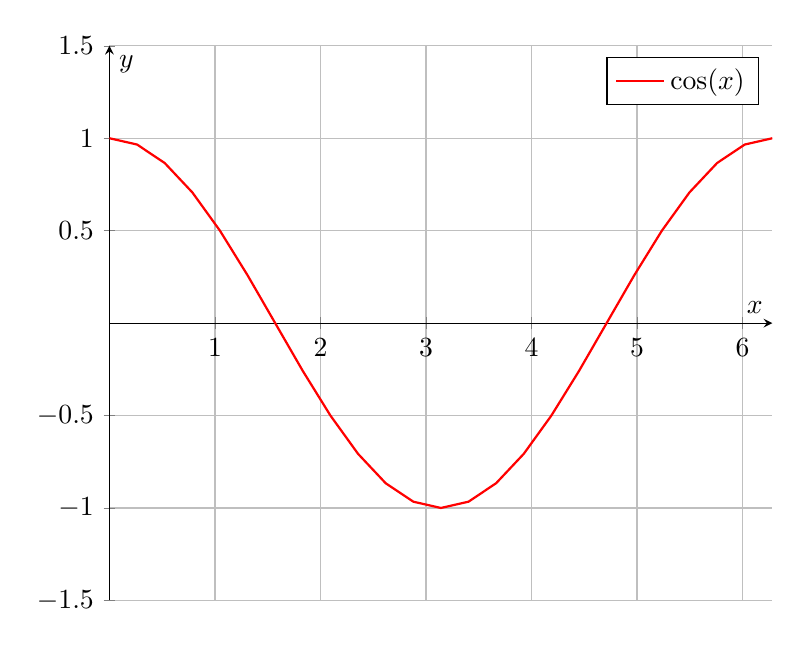
\begin{tikzpicture}
        \begin{axis}[
            axis lines = middle, 
            xlabel={$x$}, ylabel={$y$},
            domain=0:2*pi, 
            grid=both,
            xmin=0, xmax=2*pi, ymin=-1.5, ymax=1.5
        ]
            \addplot[red, thick] {cos(deg(x))};
            \legend{$\cos(x)$}
        \end{axis}
        \end{tikzpicture}
\end{figure}
\begin{align*}
\mathcal{L}[cos(wt)](s) &\stackrel{Eulero}{=} \mathcal{L}\left[\frac{e^{jwt} - e^{-jwt}}{2}\right]\\
&= \frac{1}{2}\left[\mathcal{L}[e^{jwt}](s) - \mathcal{L}[e^{-jwt}](s)\right] \\
&= \frac{1}{2}\left[\frac{1}{s-jw} + \frac{1}{s+jw}\right] \\
&= \frac{s}{s^2 + w^2}
\end{align*}
\textbf{Funzione seno}:
\begin{figure}[H]
    \centering
    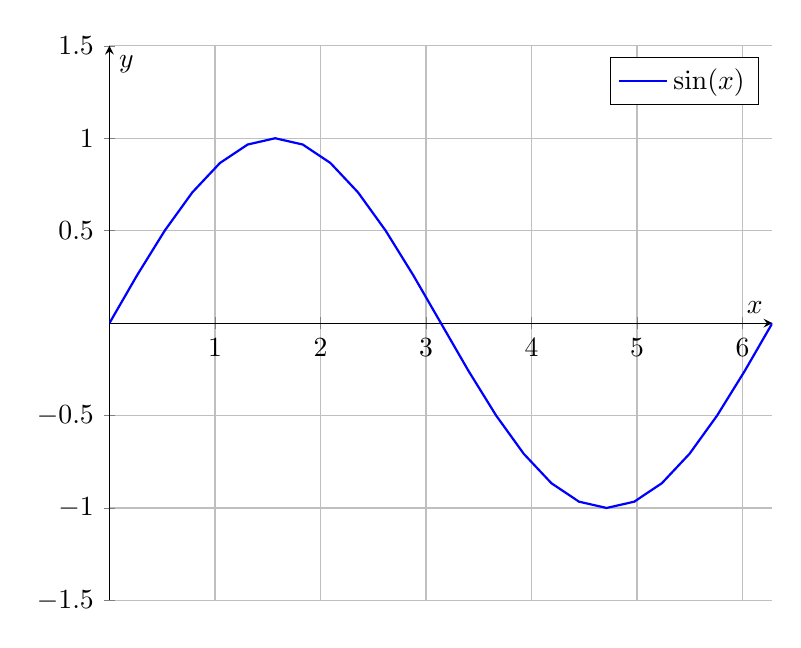
\begin{tikzpicture}
        \begin{axis}[
            axis lines = middle, 
            xlabel={$x$}, ylabel={$y$},
            domain=0:2*pi, 
            grid=both,
            xmin=0, xmax=2*pi, ymin=-1.5, ymax=1.5
        ]
            \addplot[blue, thick] {sin(deg(x))};
            \legend{$\sin(x)$}
        \end{axis}
        \end{tikzpicture}
\end{figure}
\begin{align*}
    \mathcal{L}[sin(wt)](s) &\stackrel{Eulero}{=} \mathcal{L}\left[\frac{e^{jwt} - e^{-jwt}}{2j}\right]\\
    &= \frac{1}{2j}\left[\mathcal{L}[e^{jwt}](s) - \mathcal{L}[e^{-jwt}](s)\right] \\
    &= \frac{1}{2j}\left[\frac{1}{s-jw} - \frac{1}{s+jw}\right] \\
    &= \frac{1}{2j}\left[\frac{\cancel{s}+jw - \cancel{s}+jw}{s^2 + w^2}\right] \\
    &= \frac{w}{s^2 + w^2}
\end{align*}

\subsection{Applicazione della TdL per i sistemi LTI causali}
\begin{equation*}
    \color{red}
    \sum_{i=0}^{n} a_i \frac{d^iv(t)}{dt^i} = \sum_{j=0}^{m} b_j \frac{d^ju(t)}{dt^j}
\end{equation*}
\[n \ge m \text{ e } u(t) = u(t)\cdot \delta_{-1}(t) (u(t)=0, t<0)\]
E consideriamo le n-1 condizioni iniziali:
\[v(0^-), \; \frac{dv(0)}{dt}; \; \frac{d^2v(0)}{dt^2}; \; \dots \; \frac{d^{n-1}v(0)}{dt^{n-1}}\]
Se $u(t)$ ammette TdL allora anche $v(t)$ ammette TdL e:
\begin{equation*}
    \mathcal{L}\left[\sum_{i=0}^{n} a_i \frac{d^iv(t)}{dt^i}\right](s) = \mathcal{L}\left[\sum_{i=0}^{m} b_i \frac{d^iu(t)}{dt^i}\right](s)
\end{equation*}
\begin{equation*}
    \sum_{i=0}^{n} a_i \mathcal{L}\left[\frac{d^iv(t)}{dt^i}\right](s) = \sum_{i=0}^{m} b_i \mathcal{L}\left[\frac{d^iu(t)}{dt^i}\right](s)
\end{equation*}
Applicando $n+m$ volte la regole della derivata:\\
\begin{align*}
   &a_n\left[S^nV(s) - \sum_{k=0}^{n-1}\frac{d^kv(t)}{dt^k}\bigg|_{t=0^-}(S^{n-1-k})\right] + \\
   &+ a_{n-1}\left[S^{n-1}V(s) - \sum_{k=0}^{n-2}\frac{d^kv(t)}{dt^k}\bigg|_{t=0^-}(S^{n-2-k})\right] +\\
   &+ \dots + a_0V(s)\\
   &= b_mS^mU(s) + b_{m-1}S^{m-1}U(s) + \dots + b_0U(s)
\end{align*}
Imponiamo le C.I.: $u(t)\bigg|_{t=0} = 0$\\\\
Espandiamo e raccogliamo:
\begin{align*}
    &\underbrace{\left[a_nS^n + a_{n-1}S^{n-1} + \dots + a_0\right]V(s)}_{d(s)} +\\
    &- \underbrace{a_nv(0^-)S^{n-1}\left(a_{n-1}v(0^-) + a_n\frac{dv(t)}{dt}\bigg|_{t=0^-}\right)S^{n-2} - \; \dots \; - \left(\sum_{k=0}^{n-1} a_{k+1} \frac{d^kv(t)}{dt^k}\bigg|_{t=0^-}\right)}_{p(s)}\\
    &= \underbrace{(b_mS^m + b_{m-1}S^{m-1} + \dots + b_0)}_{n(s)}U(s)
\end{align*}

\[\Longrightarrow d(s) \cdot V(s) - p(s) = n(s) \cdot U(s)\]
\[V(s) = \frac{n(s)}{d(s)} \cdot U(s) + \frac{P(s)}{d(s)}\]
\begin{itemize}
    \item \textcolor{green!70!black}{$n(s)$} è un polinonio di grado $m$
    che dipende solo dai coefficenti delle derivate associate all'ingresso. \colorbox{blue!30!white}{Polinimonio caratteristico di u(t)}
    \item \textcolor{green!70!black}{$d(s)$} è un polinomio di grado $n$ che dipende
    solo dai coefficenti delle derivate associate di uscita. \colorbox{blue!30!white}{Polinimonio caratteristico di v(t)}
    \item \textcolor{green!70!black}{$p(s):$}\[\sum_{k=0}^{n-1}S^k\left(\sum_{j=k+1}^{n} a_{j+1} \frac{d^{n-j}}{dt^{n-j}}\bigg|_{t=0^-}\right)\]
    Polinomio di grado $n-1$ che dipende solo dalle C.I di v(t)
    \item \textcolor{green!70!black}{$\frac{P(s)}{d(S)}$} è una funzione razionale che dipende solo dalle C.I ì del sistema e dai 
    coefficenti del polinomio caratteristico di $v(t)$
    \[V_l(s) = \frac{P(s)}{d(s)}\]
    \item \textcolor{green!70!black}{$\frac{n(s)}{d(s)}U(s)$} è una funzione razionale che dipende dai coefficenti
    del polinomio caratteristico di $u(t)$, dei coefficenti del polinomio caratteristico di v(t) moltiplicati per tali u(t):
    \[V_f(s) = \frac{n(s)}{d(s)}U(s)\]
\end{itemize}

\begin{examplebox}{Esempio}
    Dato un sistema LTI:
    \[\frac{d^3v(t)}{dt^3} + \frac{d^2v(t)}{dt^2} = \frac{du(t)}{dt}\]
    \[\downarrow\]
    \[\textcolor{green!60!black}{\mathcal{L}\left[\frac{d^3v(t)}{dt^3}\right]} + \textcolor{blue!80!black}{\mathcal{L}\left[\frac{d^2v(t)}{dt^2}\right]} = \textcolor{red!80!black}{\mathcal{L}\left[\frac{du(t)}{dt}\right]}\]
    \[\downarrow\]
    \[\textcolor{green!60!black}{S^3V(s) - S^2v(0^-) - S\frac{dv(0^-)}{dt} - \cancel{S^0}\frac{d^2v(0^-)}{dt^2}} +\]
    \[\textcolor{blue!80!black}{+ S^2V(s) - Sv(0^-) - \frac{dv(0^-)}{dt}} = \textcolor{red!80!black}{SU(s)}\]
    \[\underbrace{(S^3 + S^2)}_{d(s)}V(s) - \underbrace{\left[s^2v(0) + \frac{dv(0)}{dt}S + \frac{d^2v(0)}{dt^2} + v(0)S + \frac{dv(0)}{dt}\right]}_{p(s)} = \underbrace{S}_{n(s)}U(s)\]
    \[V(s) = \frac{S}{(S^3 + S^2)}U(s) + \frac{\left[s^2v(0) + \frac{dv(0)}{dt}S + \frac{d^2v(0)}{dt^2} + v(0)S + \frac{dv(0)}{dt}\right]}{S^3 + S^2}\]
\end{examplebox}
\noindent
H(s) è definita come TdL delle risposte impulsive $h(t)$. È una funzione razionale con grado del numeratore 
generalemnte minore o uguale del denominatore.
\begin{align*}
    h(t) &= d_0 \delta_0(t) + ... \left(\sum_{i=1}^{r} \sum_{l=0}^{\mu_i - 1} d_{i,l}\frac{t^l}{l!}e^{\lambda_i t}\right)\delta_{-1}(t)\\
    &\stackrel{\mathcal{L}}{=} d_0 + \sum_{i=1}^{r} \sum_{l=0}^{\mu_i - 1} \frac{d_{i,l}}{(s-\lambda)^{l+1}} = H(s)
\end{align*}
\subsubsection{Funzione di trasferimento}
    \begin{align*}
        H(s) &= \frac{\sum_{j=0}^{m}b_js^j}{\sum_{i=0}^{n}a_is^i}\\
        &= \frac{b_m(S-\beta)^{\zeta_1}(S-\beta_2)^{\zeta_2}\; ... \; (S-\beta_q)^{\zeta_q}}{a_n(S-\alpha)^{\mu_1}(S-\alpha_2)^{\mu_2}\; ... \; (S-\alpha_n)^{\mu_r}}
    \end{align*}
    \begin{center}
    \colorbox{blue!30!white}{Rapporto tra i polinomi car. di u(t) e v(t)}\\
    Dove $\alpha_i$ e $\beta_j$ sono rispettivamente radici del denominatore e del numeratore.
    \end{center}
    Possiamo anche riscriverla come:
    \[H(s) = k\frac{\prod_{i = 1}^m (S - Z_i)}{\prod_{i = 1}^n (S - P_i)} \; \;  \text{ dove } \; \; k = \frac{b_m}{a_n}\]
    Dove $(S - Z_i)$ e $(S - P_i)$ sono rispettivamente zeri e poli della funzione razionale. 
    

    \begin{definition}
        Definiamo come zero di una funzione razionale $H(s)$ un qualiasi numero $\beta \in \mathbb{C}$ t.c. $H(\beta) = 0$.
    \end{definition}
    \begin{definition}
        Definiamo come polo di una funzione razionale $H(s)$ un qualunque numero $\alpha \in \mathbb{C}$ t.c. $H(\alpha) = \infty$.
    \end{definition}
    \noindent
    Dato H(s) in forma ridotta (ho eliminato le radici in comune): Siano $\lambda_1, \; ... \; \lambda_r$ con $r \le n$ i suoi poli dopo la semplificazione
    se $Re(\lambda_i) < 0$ per $i = 1, \; ... \; r$ allora il sistema è BIBO stabile. 
    \begin{lemma}
        \label{lemma:polo_bibo_stabile}
        Un sistema è BIBO stabile se tutti i suoi poli giaciono nel semipiano complesso negativo.
    \end{lemma}
    \noindent
    Per stabilizzare un sistema (BIBO stabilizzato) devo togliere gli zeri $\lambda_i$ con $Re(\lambda_i) > 0$, dividendoli per il loro corrispettivo polo.

\begin{examplebox}{Esempio 1}
    \[v'(t) - 3v(t) = u''(t) - 5u'(t) + 4u(t)\]
    Calcoliamoci il polinomio caratteristico:
    \[s - 3 = s^2 - 5s + 4\]
    \[H(s) = \frac{n(s)}{d(s)} = \frac{\text{Pol. Car degli ingressi}}{\text{Pol. Car delle uscite}} = \frac{s^2 -5s + 4}{s - 3}\]
    \[H(s) = \frac{s^2 - 5s + 4}{s - 3} = \frac{(s-4)(s-1)}{s-3}\]
    Poiché $\lambda_1 = 3$ non è asintonticamente stabile poiché la sua parte reale è maggiore di 0.\\ Non è neanche BIBO stabile
    perché tutte le radici del denominatore (poli di $H(s)$) hanno parte reale maggiore di 0.
\end{examplebox}
\begin{examplebox}{Esempio 2}
    \[v''(t) + 3v'(t) + 2v(t) = u''(t) - 4u'(t) + 3u(t)\]
    \[H(s) = \frac{s^2 - 4s + 3}{s^2 + 3s + 2} = \frac{(s-3)(s-1)}{(s+1)(s+2)}\]
    Poiché $\lambda_1 = -1$ e $\lambda_2 = -2$ sono minori di 0 allora il sistema è asintonticamente stabile. Ricordiamo che se un sistema è 
    asintonticamente stabile allora è anche BIBO stabile.
\end{examplebox}
 \begin{examplebox}{Esempio 3}
    \[v'''(t) + 7v''(t) - 2v'(t) + 6v(t) = u''(t) + 3u(t) - 4u(t)\]
    \[H(s) = \frac{s^2 + 3s - 4}{s^3 + 7s^2 - 2s + 6} = \frac{(s+4)\cancel{(s-1)}}{\underbrace{(s+3)}_{\lambda_1 = -3}\underbrace{(s+2)}_{\lambda_2 = -2}\cancel{(s-1)}}\]
    Non è asintonticamente stabile. Tuttavia è BIBO stabile poiché tutti i poli di $H(s)$ hanno parte reale minore di 0.
 \end{examplebox}

\section{Antitrasformata di Laplace}

\[V(s) = \frac{n(s)}{d(s)} \Longrightarrow \begin{cases}
    \underbrace{deg[n(s)] \ge deg[d(s)]}_{\text{Sistema proprio}} \Longrightarrow A\\
    \underbrace{deg[n(s)] < deg[d(s)]}_{\text{Sistema strett. proprio}} \Longrightarrow B
\end{cases}\]

\begin{center}
    A $\rightarrow$ Divisione polinomiale $\rightarrow$ Fratti semplici $\rightarrow$ Antitrasformata\\
    B $\rightarrow$ Fratti complessi $\rightarrow$ Antitrasformata
\end{center}
\subsection{Divisione polinomiale}
\[V(S) = \frac{r(s)}{d(s)} + k \; \; \text{    dove    } \; \; deg[r(s)] < deg[d(s)], k \in \mathbb{C}\]
 \[\mathcal{L}[K\delta(t)] = K \stackrel{\mathcal{L}^{-1}}{\Longrightarrow} K\delta_0(t)\]
\begin{examplebox}{Esempio}
    \[V(s) = \frac{2s^2 + 4s - 3}{s^2 - s - 1} \; \; \text{ dove } \; \; m = 2, n=2\]
    \[
    \begin{array}{r|l}
    \text{Quotient} & 2 \\ \hline
    \text{Divisor} & s^2 - s - 1 \\
    \text{Step 1: } & 2s^2 + 4s - 3 \\
    \text{Subtract: } & -(2s^2 - 2s - 2) \\
    \text{Remainder: } & 6s - 1 \\
    \end{array}
    \]
    \[V(s) = \frac{6s - 1}{s^2 - s + 1} + 2\]
\end{examplebox}

\subsection{Fratti semplici}

\[\frac{r(s)}{d(s)} =  d_0 + \sum_{i=1}^{r} \sum_{l=0}^{\mu_i - 1} \frac{d_{i,l}}{(s-\lambda)^{l+1}}  \]

\begin{examplebox}{Esempio 1}
    \[V(s) = \frac{3s^2 - 1}{(s+1)^2(s-2)(s+5)}\]
    \[V(s) = \frac{A}{s-2} + \frac{B}{s+1} + \frac{C}{(s+1)^2} + \frac{D}{(s+5)}\]
    $A, B, C, D$ sono i $c_{i,l}$
\end{examplebox}
\begin{examplebox}{Esempio 2}
    \[\frac{s-20}{(s+4)(s-2)} = \frac{c_{1,0}}{(s+4)} + \frac{c_{2,0}}{s-2} = \frac{A}{s+4} + \frac{B}{s-2}\]
    \begin{enumerate}
        \item Metodo: \[\frac{A(s-2)+B(s+4)}{(s+4)(s-2)} = \frac{AS - 2A + BS + 4b}{(s+4)(s+2)}\]
        \[\begin{cases}
            A + B = 1\\
            -2A + 4B = -20
        \end{cases} \rightarrow \begin{cases}
            A = 4\\
            B = -3
        \end{cases}\] 
        \[\frac{S - 20}{(s+4)(s-2)} = \frac{4}{s+4} - \frac{3}{s-2}\]
        \item Metodo: \[c_{i,l} = \lim_{s \rightarrow \alpha_i}\frac{d^{\mu_i-l-1}\left((s-\alpha_i)^{\mu_i}\frac{r(s)}{d(s)}\right)}{ds^{\mu_i-l-1}}\]
        \[c_1  =  A = \lim_{s \rightarrow -4} \frac{\cancel{d^{1-0-1}}\left((s+4)^{1}\frac{s-20}{(s+4)(s-2)}\right)}{ds^0} = \frac{-24}{-6}= 4\]
        \[c_2  =  B = \lim_{s \rightarrow 2} \frac{d^{1-0-1}\left((s-2)^{1}\frac{s-20}{(s+4)(s-2)}\right)}{\cancel{ds^0}} = \frac{-18}{6}= -3\]
        \[\frac{S - 20}{(s+4)(s-2)} = \frac{4}{s+4} - \frac{3}{s-2}\]
    \end{enumerate}
\end{examplebox}
\noindent
Ora si applica l'antitrasformata:
\begin{align*}
    V(s) &= k + \sum_{i=1}^r \sum_{l=0}^{\mu_i - 1}\frac{c_{i,l}}{(s-\lambda_i)^{l+1}}\\
    &\stackrel{\mathcal{L}^{-1}}{=} \mathcal{L}^{-1}[k](t) + \sum_{i=0}^{r}\sum_{l=0}^{\mu_i - 1} \mathcal{L}^{-1}\left[\frac{c_{i,l}}{(s-\lambda_i)^{l+1}}\right](t)\\
    &= k\delta_0(t) +  \left[\sum_{i=0}^{r}\sum_{l=0}^{\mu_i - 1} c_{i,l} \frac{t^l}{l!}e^{\lambda_i t}\delta_{-1}(t)\right]
\end{align*}

\begin{examplebox}{Esempio completo}
    \[v''(t) - v'(t) - 2v(t) = u''(t) + 2u'(t) + u(t)\]
    \[C.I = \begin{cases}
        v(0) = 1\\
        v'(0) = 0
    \end{cases}\]
    \[u(t) = e^{3t}\delta_{-1}(t)\]
    Quello che ci viene chiesto è \begin{enumerate}
        \item Stabilità
        \item Risposta libera (nel tempo e in frequenza)
        \item Risposta impulsiva
        \item Risposta forzata
        \item Risposta totale
    \end{enumerate}
    Partiamo con il primo punto:
    \begin{enumerate}
        \item Polinomio caratteristico: $s^2 - s - 2 = 0 \rightarrow \lambda_1 = 2, \lambda_2 = -1$ e $\mu_i = 1$
        \textbf{Non è asintonticamente stabile} perché $\lambda_1 > 0$ 
        \[V(s) = \underbrace{\frac{p(s)}{d(s)}}_{V_l(s)} + \underbrace{\overbrace{\frac{h(s)}{d(s)}}^{H(s)} \cdot U(s)}_{V_f(s)}\]
        Per garantire stabilità BIBO i poli di $H(s)$ devono avere parte reale minore di 0.\\
        Calcoliamo la funzione di trasferimento:
        \[H(s) = \frac{s^2 + 2s + 1}{s^2 - s - 2} = \frac{(s+1)^{\cancel{2}}}{(s-2)\cancel{(s+1)}} = \frac{s+1}{s-2}\]
        \textbf{Non è BIBO stabile} perché $\lambda_1$ (che è un polo della funzione di trasferimento) è maggiore di 0.
        \item[2a. ] Risposta libera nel tempo:
        \begin{align*}
            v_l(t) &= \sum_{i = 1}^{r} \sum_{l = 0}^{\mu_i - 1} c_{i,l}\frac{t^l}{l!}e^{\lambda_it}\\
            &= c_{1}e^{2t} + c_{2}e^{-t}
        \end{align*}
        \[\begin{cases}
            v_l(t) = c_{1}e^{2t} + c_{2}e^{-t}\\
            v_l'(t) = 2c_{1}e^{2t} - c_{2}e^{-t}\\
        \end{cases} \stackrel{t = 0}{\rightarrow} \begin{cases}
            c_1 + c_2 = 1\\
            2c_1 - c_2 = 0
        \end{cases} \rightarrow \begin{cases}
            c_1 = 0\\
            c_2 = 1
        \end{cases}\]
        \[v_l(t) = e^{-t}\]
        
        \item[2b .] Risposta libera in frequenza:
        Facciamo la trasformata di Laplace del sistema:
         \[\mathcal{L}[v''(t) - v'(t) - 2v(t)] = \mathcal{L}[u''(t) + 2u'(t) + u(t)]\]
            \[\overbrace{(s^2V(s) - s + 1)}^{\mathcal{L}[v''(t)]} - \overbrace{(sV(s) + 1)}^{\mathcal{L}[v'(t)]} - \overbrace{2V(s)}^{\mathcal{L}[v(t)]} = (\overbrace{s^2U(s)}^{\mathcal{L}[u''(t)]} + \overbrace{2sU(s)}^{\mathcal{L}[u'(t)]} + \overbrace{U(s)}^{\mathcal{L}[u(t)]}\]
        \[\overbrace{(s^2 - s - 2)}^{\text{pol. car. uscite}}V(s) - s + 2 = \overbrace{(s^2 + 2s + 1)}^{\text{pol. car entrate}}U(s)\]
        \[V(s) = \frac{s - 2}{(s-2)(s+1)} + \frac{(s+1)^2}{(s-2)(s+1)} U(s)\]
        Vediamo ora cosa è $U(s)$:
        \[u(t) = \underbrace{e^{-3t}\delta_{-1}(t)}_{\lambda = -3, A = 1} \stackrel{\mathcal{L}}{\Longrightarrow} U(s) = \frac{1}{s+3}\]
        \[V(s) = \underbrace{\frac{1}{s+1}}_{v_l(s)} + \overbrace{\underbrace{\frac{s+1}{s-2}}_{H(s)} \cdot \frac{1}{s+3}}^{V_f(s)}\]
        Quindi la risposta libera in Laplace è: 
        \[v_l(s) = \underbrace{\frac{1}{s+1}}_{\lambda = 1, A = 1}\stackrel{\mathcal{L}^{-1}}{\Longrightarrow} e^{-t}\delta_{-1}(t)\]
        L'unica differenza che ci sta tra risposta libera e in frequenza e che quella in frequenza, quando la andiamo a trovare
        dobbiamo moltiplicarla per la funzione causale, ovvero il gradino.
        \item[3. ] Risposta impulsiva:
        \[H(s) = \frac{s+1}{s-2}\]
        Facciamo la divisione tra polinomi dove otteniamo:
        \[H(s) = 1 + \frac{3}{s-2}\]
        Applichiamo l'antitrasformata:
        h(t) = $\mathcal{L}^{-1}[H(s)] = \delta_0(t) + 3e^{2t}\delta_{-1}(t)$
        \item[4. ] Risposta forzata: Proviamo entrambi i metodi, partiamo con il primo (i fratti semplici):
        \[V_f(s) = \frac{s+1}{(s-2)(s+3)} = \frac{A}{s-2} + \frac{B}{s+3}\]
        \[\frac{As + 3A + Bs - 2B}{(s-2)(s+3)} = \frac{(A+B)s + (3A - 2B)}{(s-2)(s+3)}\]
        \[\begin{cases}
            A + B = 1\\
            3A - 2B = 1
        \end{cases} \rightarrow \begin{cases}
            A = 1 - \frac{2}{5} = \frac{3}{5}\\
            B = \frac{2}{5}
        \end{cases}\]
        \[\frac{3}{5}\frac{1}{s-2} + \frac{2}{5} \frac{1}{s+3} = \left(\frac{3}{5}e^{2t} + \frac{2}{5}e^{-3t}\right)\delta_{-1}(t)\]
        Okay ora proviamo con il metodo dei limiti:
        \[c_{i} = \lim_{s \rightarrow \lambda_i}\frac{d^{\mu - l - 1}n(s)}{ds^{s-l-1}d(s)}(s-\lambda)^\mu\]
        \[A = \lim_{S \rightarrow +2} \frac{d^{1-0-1}}{ds^{1-0-1}} \frac{s+1}{\cancel{(s-2)}(s+3)}\cancel{(s-2)} = \frac{3}{5}\]
        \[B =\lim_{S \rightarrow -3} \frac{d^{1-0-1}}{ds^{1-0-1}} \frac{s+1}{(s-2)\cancel{(s+3)}}\cancel{(s+3)} = \frac{2}{5} \]
        E come si vede, si ottiene il risultato medesimo con diverso metodo.
    \end{enumerate}
\end{examplebox}
\noindent

\section{Sistema a blocchi}

In generale ci sono tre modi per mettere a sistema un sistema a blocchi:
\begin{itemize}
    \item \textbf{Sistema in serie} (o cascata) dove l'output di un sistema A diventa l'input di un sistema B
    \[x_2 = y_1\]
    \item \textbf{Sistema parallelo} dove un input x viene separato in $x_1$ e $x_2$, entrano all'interno rispettivamente
    dei sistemi A e B e poi vengono sommati in una singola uscita $y$.
    \[x = x_1 = x_2\]
    \[y = y_1 + y_2\]
    \item \textbf{Sistema di retroazione} dove l'uscita di un sistema A diventa l'input di un sistema B e viceversa.
    \[x= x_1 + y_2 \]
    \[y = y_1 = x_2\]
\end{itemize}
I blocchi avranno sempre un singolo input e un singolo output (poiché sistemi SISO (Single Input Single Output)), per quanto riguarda i nodi sommatori,
possono entrare infiniti numeri di archi e generalmente ne esce solo una.\\
Esistono 2 tipi di controlli:
\begin{enumerate}
    \item \textit{Il controllo ad anello aperto} è un sistema in cui l'uscita non influenza l'input. È un sistema a ciclo aperto, ovvero non c'è feedback.
    \item \textit{Il controllo ad anello chiuso} è un sistema in cui l'uscita influenza l'input. È un sistema a ciclo chiuso, ovvero c'è feedback.
    Dove il sistema che ritorna il feedback del sistema A si chiama funzione di trasferimento del sistema.
\end{enumerate}
I sistemi che ci interessano di più sono quelli a ciclo chiuso, in quanto sono quelli che si avvicinano di più alla realtà.\\
Guardando la nomenclatura dei sistemi a blocchi, si ha che:
\begin{itemize}
    \item Sistema di riferimento $r$ è l'input del sistema
    \item Elemento di feedforward $F$ è un blocco che manda un segnale di controllo al processo
    \item Processo $P$ è il sistema che trasforma l'input in un output (che però può essere disturbato)
    \item Elemento di feedback $B$ è un blocco che manda un segnale di feedback $b$ al processo per correggere l'errore 
    \item Segnale di attuazione che è in genere una sorta di errore $e = r - b$ (in genere viene chiamato 
    chiamato feedback negativo quando $e = r-b$ mentre è feedback positivo quando $e = r + b$)
\end{itemize}

\subsection{Controllori}
I controllori sono di tre tipi con relative regole di controllo:
\begin{itemize}
    \item P è il controllore proporzionale e la sua regola di controllo è $u(t) = K_p e(t)$
    \item I è il controllore integrale e la sua regola di controllo è $u(t) = K_i \int e(\tau)d\tau$
    \item D è il controllore derivativo e la sua regola di controllo è $u(t) = K_d \frac{de(t)}{dt}$
\end{itemize}
Possiamo anche combinarli insieme, esistono tipi "compositi" di controllori come PID, PI, PD, I, P, D.
\[\mu_{pid} = K_p e(t) + K_d \frac{de(t)}{dt} + K_i \int e(t)dt\]
Quando abbiamo un sistema a blocchi complesso e ridurlo a un sistema a blocchi più semplice, applicando diverse regole di riduzione:
\subsection{Forma canonica - nomenclatura}
La \textbf{Forma canonica} è una forma standard di rappresentazione di un sistema a blocchi.
\begin{enumerate}
    \item $G$: Funzione di trasferimento diretta
    \item $H$: Funzione di trasferimento di feedback
    \item $GH$: Funzione di trasferimento del loop (o anello)
    \item $\frac{C}{R}$ = Funzione di trasferimento dell'anello chiuso 
    \[\frac{C}{R} = \frac{G}{1 \pm GH} = \frac{\text{eq. car. dell'ingresso}}{\text{eq. car. dell'uscita}}\]
    \item $\frac{E}{R}$: rapporto del segnale di attuazione $ = \frac{1}{1 \pm GH}$
    \item $\frac{B}{R}$: rapporto di feedback $ = \frac{GH}{1 \pm GH}$ 
\end{enumerate}
L'obiettivo è di compattare il sistema fino ad arrivere ad un sistema a blocchi uguale alla forma canonica.
Prendiamo per esempio il sistema massa molla smorzatore:
\begin{align*}
    ma &= \sum F\\
    mx'' &=  F_{ext} - kx - bx'\\
    F_{ext} &= kx + bx' + mx''\\
    F_{ext}(s) &= kX(s) + bsX(s) + ms^2X(s)\\
    X(s) &= \frac{F_{ext}(s)}{ms^2 + bs + k}
\end{align*}

\subsection{Regole di trasfromazione}

\begin{enumerate}
    \item \textbf{Combinazione di blocchi in serie}: dati due blocchi $A$ e $B$ in serie, riducendolo otteniamo un singolo blocco che è il prodotto di $AB$.
    \item \textbf{Combinazione di blocchi in parallelo}: dati due blocchi $A$ e $B$ in parallelo, riducendolo otteniamo un singolo blocco che è (in base al sommatore) $A\pm B$.
    \item \textbf{Rimozione di blocchi in parallelo}: dati due blocchi $A$ e $B$ in parallelo, riducendolo otteniamo un singolo blocco che è il prodotto di $AB$ diviso la somma di $AB$.
    \item \textbf{Rimozione di anello feedback}: dati due blocchi $A$ e $B$ in feedback, riducendolo otteniamo un singolo blocco che diventa $\frac{A}{1 \pm AB}$
    \item \textbf{Rimozione del loop}: dati due blocchi $A$ e $B$ in loop, possiamo spostare il blocco retroattivo all'inizio del blocco iniziale
    \item \textbf{Riorganizzazione degli input}: posso organizzare gli input del sistema a blocchi come voglio, l'importante è che alla fine si arrivi ad un sistema a blocchi canonico.
    \item \textbf{Spostamento dei nodi di somma prima di un blocco}: posso spostare i nodi di somma prima di un blocco
    \item \textbf{Spostamento dei nodi di somma dopo un blocco}: posso spostare i nodi di somma dopo un blocco
    \item \textbf{Spostamento dei nodi prima di un blocco}: posso spostare i nodi prima di un blocco
    \item \textbf{Spostamento dei nodi dopo un blocco}: posso spostare i nodi dopo un blocco
\end{enumerate}

\section{Diagrammi di flusso}

I diagrammi di flusso sono una rappresentazione grafica di un sistema a blocchi. 
\\
Guardiamo ora le diverse componenti di un diagramma di flusso:
\begin{itemize}
    \item \textbf{Percorso in avanti:} Un cammino che unisce un nodo di input ad un nodo di output
    \item \textbf{Percorso ad anello:} Un cammino che inizia e finisce nello stesso nodo e senza passare più volte in altri nodi intermedi
    \item \textbf{$\rightarrow$ Self loop:} Un cammino che inizia e finisce nello stesso nodo e non tocca altri nodi intermedi
    \item \textbf{Guadagno}: prodotto di tutti i pesi degli archi lungo un percorso
\end{itemize}

\subsection{Convertire un Sistema a blocchi in un diagramma di flusso}

Per convertire un sistema a blocchi in un diagramma flussi (così che sia più facile da gestire) dobbiamo convertire gli archi e i nodi nel seguente modo:

\begin{enumerate}
    \item Indiviiamo i nodi di input e output
    \item Per ogni nodo somma si aggiunge un nodo 
    \item Per ogni nodo dello schema a blocchi si aggiunge un nodo al diagramma di flusso
    \item Unisco i nodi con gli archi il cui peso è la funzione dentro al blocco. Se tra un nodo e l'altro non ci sono blocchi, il suo peso vale 1.
\end{enumerate}

\subsection{Funzione di Mason}

\begin{definition}
    La funzione di Mason è una funzione che permette di calcolare la funzione di trasferimento di un sistema a blocchi.
    \[T = \sum_i \frac{P_i \Delta_i}{\Delta} \]
    dove 
    \begin{itemize}
        \item $P_i$ è il guadagno del percorso i
        \item $\Delta_i$ è il determinante del percorso i
        \item $\Delta$ è il determinante del sistema
        \begin{align*}
            \Delta &= 1 - (-1)^{k+1} \sum_k \sum_j P_{jk}\\
            &= 1 - \left(\sum_j P_{j1} + \sum_j P_{j2} + ... \right)\\
            &= 1 - \left(\parbox{5cm}{Somma dei guadagni di tutti gli alberi}\right) + \left(\parbox{4cm}{Somma dei dei guadagni\\dei prodotti degli anelli\\che non toccano a due}\right) \\
            &+ \left(\parbox{5cm}{somma dei guadagni dei prodotti degli anelli che non si toccano 3 a 3}\right) + ...
        \end{align*}
    \end{itemize}       
\end{definition}

\begin{examplebox}{Esempio 1}
    Prendiamo come esempio il diagramma di flusso visto a lezione (guarda gli punt) e calcoliamo la funzione di Mason.
    Troviamo i guadagni per ogni percorso:
    \[P_1 =(x_1, x_2, x_3, x_4) = 1 \cdot G \cdot 1 =  G\]
    \[P_{1,1} = (x_2, x_3) = -GH\]
    L'ordine in cui vengono chiamati i percorsi è arbitrario. Sono stati scelti semplicemente nell'ordine in cui li abbiamo notati.
    I guadagni che hanno 1 non vengono considerati.
    Calcoliamo ora il determinante del sistema:
    \[\Delta = 1 - (P_{1,1}) = 1 + GH\]
    Annulo tutti gli archi che toccano il percorso i-esimo:
    \[\Delta_1 = 1 - \cancel{P_{1,1}} = 1 - 0 = 1\]
    \[T = \frac{P_1 \Delta_1}{\Delta} = \frac{G \cdot 1}{1 + GH} = \frac{G}{1 + GH}\]
\end{examplebox}

\begin{examplebox}{Esempio 2}
    TODO\dots
    \begin{table}[H]
        \begin{tabular}{|c|c|c|c|c|c|c|c|c|c|c|c|}
            \hline
            & Anelli & $x_1$ & $x_2$ & $x_3$ & $x_4$ & $x_5$ & $x_6$ & $x_7$ & $x_8$ & $x_9$ & $x_{10}$\\
            \hline
            $A_1^1$ & -AB &  &  & 1 & 1 &  &  &  &  &  & \\
            \hline
            $A_2^1$& -CD & &  &  &  & &  & 1 & 1 & 1 & \\
            \hline
            $A_3^1$ & FCE & 1 & 1 &  &  &  & 1 & 1 & 1 & 1 & \\
            \hline
            $A_4^1$ & FGE & 1 & 1 &  &  &  & 1 & 1 & 1 & 1 & 1\\
            \hline
            $A_5^1$& ACE & 1 & 1 & 1 & 1 & 1 & 1 & 1 & 1 & 1 & 1\\
            \hline
            $A_6^1$ & AGE & 1 & 1 & 1 & 1 & 1 & 1 &  & 1 & 1 & 1\\
            \hline
        \end{tabular}
    \end{table}
\end{examplebox}

\section{Diagrammi di Bode}

I diagrammi di Bode sono un modo per rappresentare graficamente la risposta in frequenza di un sistema.

\begin{examplebox}{Esempio}
    \begin{align*}
        u(t) &= \sin\left(\frac{1}{2}t\right)\\
        &= \frac{1}{2}\frac{rad}{s}\alpha Hz
    \end{align*}
    
    \begin{align*}
        v(t) &= 2u(t) + \int u(t)dt\\
        &= 2sin\left(\frac{1}{2}t\right) + \int sin\left(\frac{1}{2}t\right)dt\\
        &= 2sin\left(\frac{1}{2}t\right) - 2cos\left(\frac{1}{2}t\right)\\
        &= \sqrt{2^2+2^2} \sin\left(\frac{1}{2}t + a\tan\left(\frac{-2}{2}\right)\right)\\
        &= 2.83 \sin\left(\frac{1}{2}t - 0.785\right)\\
        &= A \sin(\omega t + \phi)
    \end{align*}
\end{examplebox}
\noindent
Questo diagramma ci aiuta a capire come si comporta un sistema descritto da segnali
\textbf{sinusoidali}. 
\subsection{Motivo delle sinusoidi}
I sistemi descritti da segnali sinusoidali sono utili perchè
vedremo che qualsiasi segnale può essere rappresentato come una somma di sinusoidi.

\vspace{1em}
\noindent
Un sistema LTI causale permette le seguenti operazioni:
\begin{itemize}
  \item \( u(t) \cdot a \) 
  \item \( \frac{d u(t)}{t} \) 
  \item \( \int u(t) \,dt \) 
  \item \( u_1(t) + u_2(t) \) 
\end{itemize}
L'output del sistema è un onda scalata rispetto all'ampiezza o ritardata rispetto al
tempo:

\begin{examplebox}{Esempio}
  Prendiamo ad esempio il seguente sistema:
  \[
  \begin{aligned}
    u(t) &= \sin(\frac{1}{2}t)\\
    \omega &= \frac{1}{2} \frac{rad}{s} \alpha Hz
  \end{aligned}
  \] 
  Calcoliamo l'ingresso:
  \[
  \begin{aligned}
    v(t) &= 2 \cdot u(t) + \int u(t) \,dt\\
         &= 2 \sin(\frac{1}{2}t) + \int \sin(\frac{1}{2}t) \,dt\\
         &= 2 \sin(\frac{1}{2}t) - 2 \cos(\frac{1}{2}t)
  \end{aligned}
  \] 
  Utilizziamo un'\textbf{identità trigonometrica}, cioè:
  \[
    \begin{aligned}
      \color{red}a \color{black} sin(x) + \color{red} b \color{black} cos(x) =\\
      = \sqrt{a^2 + b^2} \cdot \sin(x + \rho )
    \end{aligned}
  \] 
  dove: \( \rho = atan\left(\frac{b}{a}\right) \quad a \ge 0 \) 
  \[
  \begin{aligned}
    v(t) &= \overbrace{2}^{a} \sin(\overbrace{\frac{1}{2}t}^{x}) \overbrace{- 2}^{b} \cos(\frac{1}{2}t)\\
         &= \sqrt{2^2 + (-2)^2} \cdot  \sin\left(\frac{1}{2}t + atan\left(\frac{-2}{2}\right)\right)\\
         &= \sqrt{8} \cdot  \sin\left(\frac{1}{2}t + atan(-1)\right)\\
         &= 2.83 \cdot \sin\left(\frac{1}{2}t - 0.785\right)\\
         &= A \cdot \sin(\omega + \phi)
  \end{aligned}
  \] 
\end{examplebox}

\subsection{Rappresentazione del diagramma di Bode}
Il diagramma di bode permette di rappresentare il comportamento di un sistema LTI formato 
da sinusoidi, di seguito guardiamo un diagramma semi-logaritmico 
(cioè con un asse lineare e uno logaritmico) che rappresenta l'ampiezza e la fase di un
sistema LTI:

\vspace{1em}
\noindent
\textbf{Osservazione}:

\noindent
  Il decibel \( dB \) è un unità di misura inventata nel 1920 per misurare quanto si
  disperde il segnale acustico su una transmission unit (\( 1TU = 10 \log_{10} \Delta_{\text{Potenza}} \)).
  Quindi un decibel è il minimo di potenza che un orecchio umano può percepire.
  \[
    \text{Potenza} = \text{Ampiezza}^2
  \] 
  \[
    1 bel = 1 TU = 10\log_{10} A^2 = 20 \log_{10} A
  \] 
  \[
    1 dB = \frac{1}{10} bel
  \] 

  \begin{examplebox}{Esempio}
    \[
      \begin{aligned}
        u(t) &= \sin(\frac{1}{2}t) \quad \omega = \frac{1}{2}\\
        v(t) &= 2.83 \cdot \sin\left(\frac{1}{2}t - 0.785\right)\\
      \end{aligned}
    \] 
    Studiamo il sistema in frequenza:
    \label{05-12-D4}
    \[
      \begin{aligned}
        V(s) &= \left( 2 + \frac{1}{s} \right) U(s)\\
        \frac{V(s)}{U(s)} &= 2 + \frac{1}{s} = \frac{2s + 1}{s} \quad \text{Funzione di trasferimento del sistema}\\
      \end{aligned}
    \] 
    \( s \) è un numero complesso:
    \[
      s = \sigma + j \omega
    \] 
    Con la risposta in frequenza la \( s \) diventa solo \( s = j \omega \), quindi
    otteniamo:
    \[
      \begin{aligned}
        \frac{V(s)}{U(s)} &= \frac{2j\omega + 1}{j\omega}\\
                          &= \frac{2 \cancel{j \omega}}{\cancel{j \omega}} + \frac{1}{j \omega} \cdot \frac{j}{j}\\
                          &= 2 - \frac{1}{\omega} \cdot j\\
      \end{aligned}
    \] 
    La rispsota del sistema nel piano dei complessi è:
    \label{05-12-D5}
    dove:
    \[
      \begin{aligned}
        \text{Ampiezza} &= l = \sqrt{\Re^2 + \Im^2}\\ 
        \text{Fase} &= \theta = atan2\left( \Im, \Re \right)
      \end{aligned}
    \]
    \[
      atan2(\sigma ,j \omega) =
      \begin{cases}
        atan \left( \frac{\omega}{\sigma } \right) & \text{se } \sigma > 0,\;\; \omega \in \mathbb{R}\\
        segno(\omega) \cdot \frac{\pi}{2} & \text{se } \sigma = 0,\;\; \omega \neq 0\\
        atan \left( \frac{\omega}{\sigma } \right) + \pi \cdot segno(\omega) & \text{se } \sigma < 0,\;\; \text{ o } \sigma =0\;\; \omega \ge  0
      \end{cases}
    \] 
    Il diagramma di Bode sarà:
  \end{examplebox}

\subsection{Risposta in frequenza}

\[u(t) = Ae^{\omega_0 + \phi} \Longrightarrow Ae^{j\phi}e^{j\omega_0t} \Longrightarrow LTI{BIBO} \Longrightarrow v(t)\]

\[A \in \mathbb{R}_+ \; \;\phi,\omega \in \mathbb{R}\]
\begin{align*}
    H(j\omega) &:= \int_{-\infty}^{+\infty} h(\tau)e^{-j\omega t}d\tau \; \; \text{per ogni } \omega \in \mathbb{R}\\
    &:= \mathcal{L}[h(t)]\bigg|_{s = j\omega}(s)\\
\end{align*}
\noindent
Prendiamo come esempio un fasore:
\[u(t) = Ae^{j\phi}e^{j\omega t}\] 
\[u(t) \rightarrow [h(t)] \rightarrow v(t)\]
\begin{align*}
    v(t) &= \int_{-\infty}^{+\infty} h(\tau)u(t-\tau)d\tau\\
    &= \int_{-\infty}^{+\infty} h(\tau)Ae^{j\phi}e^{j\omega(t-\tau)}d\tau\\
    &= Ae^{j\phi}e^{j\omega t}\int_{-\infty}^{+\infty} h(\tau)e^{-j\omega \tau}d\tau\\
    &= Ae^{j\phi}e^{j\omega t}H(j\omega) = Ae^{j\phi}e^{j\omega t}A(\omega)e^{j\phi(\omega)}\\
    &= AA(\omega)e^{j(\phi + \phi(\omega))}e^{j\omega t}
\end{align*}
Dove $A$ è l'ampiezza di $u(t)$, $A(\omega)$ è l'ampiezza della risposta in frequenza, $\phi$ è la fase di $u(t)$ e $\phi(\omega)$ è la fase della risposta in frequenza, $\omega$ è la frequenza iniziale e 
rimane invariata.
\textit{Bode ci serve a capire il comportamento del sistema al variare della frequenza del segnale d'ingresso.} Che sia un fasore o una sinusoide ci dice cosa succede se aumentiamo o diminuiamo la frequenza del nostro segnale d'ingresso.


\subsection{Operazioni tra numeri complessi}

\begin{property}
    Siano $a$ e $b$ due numeri complessi, allora:
    \begin{itemize}
        \item $|ab| = |a||b|$
        \item arg$(ab)$ = arg$(a)$ + arg$(b)$
        \item  $|a / b| = |a| / |b|$
        \item arg$(a / b)$ = arg$(a)$ - arg$(b)$
        \item $|a^n| = |a|^n$
        \item arg$(a^n)$ = n arg$(a)$
    \end{itemize}
\end{property}
\begin{property}
    Sia $s$ un numero complesso con $x \in \mathbb{C} t.c.:$
    \[\log s = x \Longleftrightarrow s = e^x\]
    E scrivendo S in forma esponenziale e x in forma complessa:
    \[S = \rho e^{j\omega} \; \; x = \sigma + j\omega\]
    \begin{align*}
        \log s &= x\\
        &= \log \rho + j\phi\\
        &= \log |s| + j arg(s)
    \end{align*}
\end{property}

\subsection{Forma di Bode}

\begin{align*}
    H(s) &= \frac{{\sum_j b_j S^j}}{{\sum_i a_i S^i}}U(s)\\
    &= K\frac{(s-z_1)^{\mu_1} \dots (s - z_e)^{\mu_e}}{(s-p_1)^{\gamma_1} \dots (s - z_r){^\gamma_r}}
\end{align*}
Molteplicità delle soluzioni algebriche:
\[l \le m, \mu_1 + \dots + \mu_e = m\]
\[r \le n, \gamma_1 + \dots + \gamma_r = n\]
\begin{theorem}
    La forma di Bode di un sistema LTI è:
\begin{align*}
    H(s) &= K_b \frac{\prod_i (1 + s\tau_i')^{\mu_i'} \prod_k \left(1 + 2\zeta_k' \frac{s}{\omega_{n,k}'} + \frac{s^2}{(\omega_{n,k}^2)}\right)^{\mu_k'}}{(S^{r_1})\prod_i (1 + s\tau_i)^{\mu_i} \prod_k \left(1 + 2\zeta_k \frac{s}{\omega_{n,k}} + \frac{s^2}{(\omega_{n,k}^2)}\right)^{\mu_k}}
\end{align*}
\begin{itemize}
    \item[] $K_b$: è il termine costante (o guardagno di Bode)
    \item[] $S^r$: raggruppa tutti le radici nulle
    \item[] $(1+s\tau_i)^{\mu_i}$: raggruppa la singola radice reale 
    \item[] $\left(1 + 2\zeta_k \frac{s}{\omega_{n,k}} + \frac{s^2}{(\omega_{n,k}^2)}\right)^{\mu_k}$: raggrupa la singola radice complessa coniugata
\end{itemize}
\end{theorem}
Per arrivare a questa forma dobbiamo raccogliere le "costanti":
\begin{examplebox}{Esempio}
    \[H(s) = 4\frac{s^3+s^2-2s}{s^3+s^2}\]
    \begin{enumerate}
        \item Poli/Zeri Nulli
        \[H(s) = 4 \frac{s(s+2)(s-1)}{s^2(s+1)} = 4 \frac{1}{2} \frac{s^2+s-2}{s+1}\]
        \item Poli e zeri reali e cerco di arrivare alla forma di bode: $(1 + s\tau)^{\mu}$
        \begin{align*}
            H(s) &= 4\frac{1}{s}\frac{s^2+s-2}{s+1}\\
            &= 4\frac{1}{s}\frac{(s+2)(s-1)}{s+1}\\
            &= 4\frac{1}{s} \frac{-(1 - s)2\left(1 + \frac{s}{2}\right)}{(1 + s)} \\
            &= \frac{-8}{1} \frac{1}{s} \frac{(1-s)\left(1-\frac{s}{2}\right)}{1+s}\\
            &= -8 \frac{1}{s} \frac{(1-s)\left(1 + \frac{s}{2}\right)}{1+s}\\
            &= -8 \frac{1}{s} \frac{(1 - s) + \left(1 + \frac{s^2}{2}\right)}{1+s}\\
            &= K_b \frac{1}{s^\mu} \frac{(1+s\tau_1)^{\mu_i} (1+s\tau_2)^{\mu_2}}{(1+s\tau_1)^{mu_1}}
        \end{align*}
        \item Polo o zero complesso coniugato
        \begin{align*}
            &= (s-(\sigma + j\omega))(s-(\sigma - j\omega)) = s^2 - 2\sigma s + \sigma^2 + \omega^2\\
            &= (s^2-s\sigma + sj\omega - s\sigma - sj\omega + |z|^2)\\
            &= (s^2 - 2s\sigma + |z|^2)^\mu\\
            &= |z|^{2\mu} \left(1 - 2\frac{2\sigma}{|z|^2}s + \frac{s^2}{|z|^2}\right)^\mu\\
            &= |z|^{2\mu} \left(1 -2\zeta\frac{s}{\omega_n} + \frac{s^2}{\omega_n^2}\right)^\mu
        \end{align*}
        dove $\zeta = \frac{-\sigma}{|z|} = -\frac{-Re(z)}{|z|}$ è il coeff. di smorzamento e $w_n = |z|$ ovvero la pulsazione naturale.
    \end{enumerate}
\end{examplebox}
\noindent
Dobbiamo trasformare $H(s) \rightarrow H(j\omega)$: Analisi in frequenza
\[H(j\omega) = K_b \frac{\prod_i (1 + j\omega\tau_i')^{\mu_i'} \prod_k \left(1 + j2\zeta_k' \frac{j\omega}{\omega_{n,k}'} - \frac{(j\omega)^2}{(\omega_{n,k}^2)}\right)^{\mu_k'}}{(S^{r_1})\prod_i (1 + j\omega\tau_i)^{\mu_i} \prod_k \left(1 + j2\zeta_k \frac{j\omega}{\omega_{n,k}} - \frac{(j\omega)^2}{(\omega_{n,k}^2)}\right)^{\mu_k}}\]
\begin{examplebox}{Esempio 2}
    
    \begin{align*}
        H(s) &= \frac{s^2-2s^2-8s}{s^4 - 2s^3 + 2s^2} = \frac{s(s^2-2s-8)}{s^2(s^2-2s+2)} = \frac{s^2-2s-8}{s(s^2-2s+2)}\\
        &= \frac{(s-4)(s+2)}{s(s^2-2s+2)}\\
        &= \frac{-4\left(1 - \frac{s}{4}\right)\cancel{2}\left(1 + \frac{s}{2}\right)}{s\cancel{(2)}\left(1 - s + \frac{s^2}{2}\right)} = -4\frac{1}{s}\frac{\left(1 - \frac{s}{4}\right)\left(1 + \frac{s}{2}\right)}{\left(1 - s + \frac{s^2}{2}\right)}\\
    \end{align*}
    Ora vediamo ogni singolo $(1 + s\tau)^{\mu}$:
    \begin{itemize}
        \item $\left(1 - \frac{s}{4}\right)$ dove $\tau_1 = -\frac{1}{4}$
        \item $\left(1 + \frac{s}{2}\right)$ dove $\tau_2 = \frac{1}{2}$
        \item $\left(1 - s + \frac{s^2}{2}\right)$ dove $w_n^2 = 2 \rightarrow w_n = \sqrt{2}$
        \[\frac{2\zeta}{w_n} = -1 \Longrightarrow \frac{2\zeta}{\sqrt{2}} = -1 \Longrightarrow \zeta = \frac{-1\sqrt{2}}{2} = -\frac{\sqrt{2}}{2}\]
    \end{itemize}
   
\end{examplebox}

\subsubsection{Quattro possibili diagrammi di Bode}

\begin{enumerate}
    \item Terminte costante $K_b$
    \item Uno zero o un polo nullo $S^\mu$ dove $\mu$ è la moltepliicità
    \item Polo o zero reale $(1 + s\tau)^{\mu}$
    \item Polo o zero complesso coniugato $\left(1 + 2\zeta \frac{s}{\omega_n} + \frac{s^2}{\omega_n^2}\right)^\mu$
    dove $\zeta$ è il coeffiicente di smorzamento e $\omega_n$ è la pulsazione naturale.
\end{enumerate}
Partiamo dal primo:
\begin{enumerate}
    \item  \[A = |H(j\omega) = |K_b|\]
     Un numero reale ha 2 fasi:
    \[\phi = atan2(\sigma + j\omega) = \begin{cases}
        0\degree & \text{se } \sigma > 0\\
        -180\degree & \text{se } \sigma < 0 
    \end{cases}\]
    \item Polo nullo 
    con $\mu \in \mathbb{Z}, \mu > 0$ zero, $\mu < 0$ polo
    \[H(s) = H(j\omega) = (j\omega)^{\mu}\]
    Consideriamo l'ampiezza di $H(j\omega)$:
    \[|H(s)| = |(jw)^\mu| = |\omega|^\mu = \omega^\mu\]
    \begin{align*}
        A(\omega) = |H(j\omega)|_{dB} &= 20\log_{10} \omega^\mu = 20\mu \log_{10} \omega\\
    \end{align*}
    Questa è una rette che cresce/decresce di $20\mu$ dB/decade.
    Cosa succede invece alla fase?
    \[\phi(\omega) = atan2(j\omega)^{\mu} = \mu \cdot atan2(j\omega) = \mu 90\degree\]
    Retta costante che passa per per $\mu$ di $90\degree$. Consideriamo i seguenti zeri e poli di $H(j\omega)$:
    \begin{table}[H]
        \centering
        \begin{tabular}{c|c|c|c}
            $\omega$ & $S^1$ & $S^{-1}$ & $S^{-2}$\\
            \hline
            $10^{-2}$ &-40 & 40 & 80\\
            $10^{-1}$ &-20 & 20 & 40\\
            $10^0$ & 0 & 0 & 0\\
            $10^1$ & 20 & 20 & 40\\
            $10^2$ & 40 & -40 & 80\\
        \end{tabular}
    \end{table}
    \item Zeri e poli reali 
    \\
    I poli possono essere scritti così:
    \[\frac{1}{1+\frac{s}{\omega_0}} = \frac{1}{1+  \tau s}\]
    \[\omega_0 = \frac{1}{|\tau|}\]
    \[A(\omega) = 20\log_{10} (\sqrt(\Re^2 + \Im^2))\]
    \[\phi(\omega) = atan2(\Im , \Re)\]
    \begin{table}[H]
        \centering
        \begin{tabular}{c|c|c}
            $\omega < \omega_0$ & $\omega = \omega_0$ & $\omega > \omega_0$\\
            \hline
            $A(\omega) = 20\log_{10} 1 = 0$ & $A(\omega) = 20\log_{10} \sqrt{-2} = -3db$ & $A(\omega) = 20\log_{10} \sqrt{\omega^2\tau^2 + 1} = 20db$\\
            $\phi(\omega) = atan2(1) = 0$ & $\phi(\omega) = atan2(2) = -45\degree$ & $\phi(\omega) = atan2(\omega\tau) = -90\degree$\\
        \end{tabular}
    \end{table}
    \item Poli e zeri complessi coniugati
    \[H(s) = \left(1 + 2\zeta\frac{\omega}{\omega_n} + \frac{\omega^2}{\omega_n^2}  \right)^{\mu}\]
    Partiamo del caso di un polo:
    \[H(s) = \frac{\omega_0^2}{s^2 + 2\zeta\omega_0s+ \omega_0^2} \stackrel{\text{Bode}}{\Longrightarrow} \frac{1}{1 + 2\zeta\frac{s}{\omega_0} + \frac{s^2}{\omega_0^2}} \stackrel{s=j\omega}{\Longrightarrow} \frac{1}{1 +2j\omega\frac{\omega}{\omega_0} + \frac{\omega^2}{\omega_0^2}}\]
    Fattorizziamo:
    \[\Re = \frac{1 - \left(\frac{\omega}{\omega_0}\right)^2}{\left(1- \left(\frac{\omega}{\omega_0}\right)^2\right)^2 + \left(2\zeta\frac{\omega}{\omega_0}\right)^2}\]
    \begin{itemize}
        \item Se $\omega << \omega_0$
        \[A(\omega) = -20\log_{10}(1) = 0\]
        \[\phi(\omega) = atan2(0) = 0\degree\]
        \item Se $\omega >> \omega_0 = \omega_n$
        \[A(\omega) = -20\log_{10} \left(\frac{\omega}{\omega_0}\right)^2 = -40\log \left(\frac{\omega}{\omega_0}\right)\]
        È una retta che decresce di 40db/decade
        \[\phi(\omega) = atan2\left(2\zeta\frac{\omega}{\omega_0}\right) = -180\degree\]
        \item $\omega = \omega_0 = \omega_n$
        Per $\zeta \ge 0.5$:
        \[A(\omega) = -20\log_{10} (2\zeta) = 0\]
        Il grafico passa per $\omega_0$, ma se $\zeta <0.5$? Picco di risonanza.
        Se $\zeta = 0$ c'è discontinuità.
        \[\phi(\omega)  = -90\degree\]
        In generali le fomule per calcolare l'ampiezza di un polo o zero complesso coniugato sono:
        \begin{itemize}
            \item $\omega >> \omega_0$
            \[A(\omega) = -20\log_{10} \left(\frac{\omega}{\omega_0}\right)^2 = -40\log_{10} \left(\frac{\omega}{\omega_0}\right)\]
            \[\phi(\omega) = \mu sgn(\zeta) = -180\degree\]
            \begin{itemize}
                \item $\zeta = 0$ asintoto verticiale in $A(\omega)$ in $\omega_n$
                \item $0 < \zeta \le 0.5$ picco di risonanza, per cui la pulsazione naturale: $\omega_r = \omega_n\sqrt{1-2\zeta^2}$ e l'ampiezza del picco: $M_r = 20\mu\log_{10}(2\zeta\sqrt{1-\zeta^2})$
                \item $\zeta = 0.5$ $A(\omega) = 0$
                \item $0.5 > \zeta > 1$ "Passa sotto" il grafico asintotico
            \end{itemize}
        \end{itemize}
    \end{itemize}
\end{enumerate}

\begin{examplebox}{Esempio}
    \[H(s) = \frac{s^2(s+1)(s^2+3s+16)}{(2s-1)}\]
    \begin{enumerate}
        \item Portare la funzione di trasferimento in forma di Bode. Se si dovessero trovare trinomi scomponibili, ricordarsi di scomporli. In questo caso
        il trinomio al denominatore ha soluzioni coniugate complesse e quindi non lo andremo a scomporre.
        \begin{align*}
            H(s) &= \frac{s^2(1)\left(1+\frac{s}{1}\right)^1(16)\left(1 + \frac{3}{16}s + \frac{s^2}{16}\right)^1}{-(1 - 2s)^1}\\
            &= -16 \frac{s^2(1+s)\left(1 +\frac{3}{16}s + \frac{s^2}{16}\right)}{(1-2s)}
        \end{align*}
        \item Cominciamo a calcolare i diagrammi di Bode dei diversi termini:
        \begin{itemize}
            \item $K_b = -16$: 
            \[A = 20\log_{10} (|-16|) = 24\]
            \[\phi = \begin{cases}
                0\degree & \text{ se } K_b > 0\\
                -180\degree & \text{ se } K_b < 0
            \end{cases}\]
            Quindi $\phi = -180\degree$
            \begin{figure}[H]
                % Amplitude plot
                \centering
            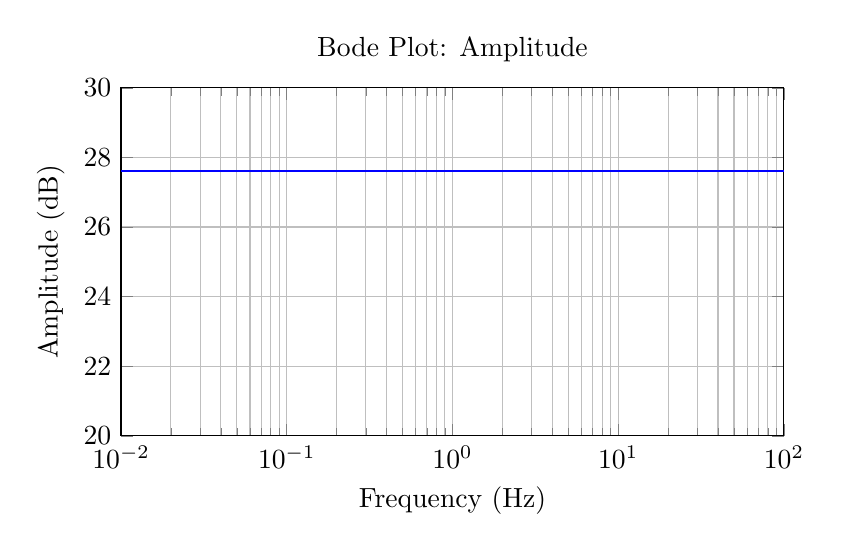
\begin{tikzpicture}
                \begin{semilogxaxis}[
                    title={Bode Plot: Amplitude},
                    xlabel={Frequency (Hz)},
                    ylabel={Amplitude (dB)},
                    grid=both,
                    xmin=1e-2, xmax=1e2,
                    ymin=20, ymax=30,
                    width=10cm,
                    height=6cm
                ]
                    % Amplitude plot
                    \addplot[
                        thick,
                        blue
                    ]
                    coordinates {
                        (1e-2, 27.6) (1e-1, 27.6) (1, 27.6) (10, 27.6) (1e2, 27.6)
                    };
                \end{semilogxaxis}
            \end{tikzpicture}
            \end{figure}
            \begin{figure}[H]
                \centering
                % Phase plot
                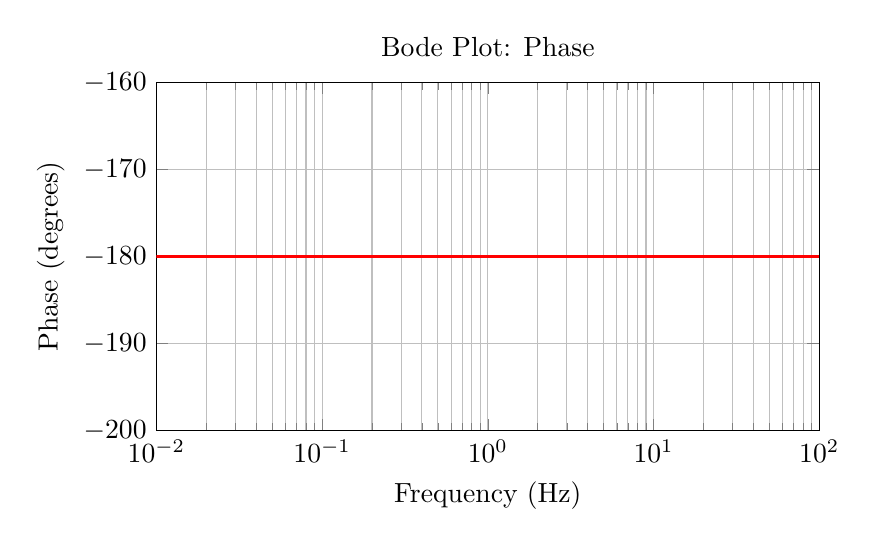
\begin{tikzpicture}
                    \begin{semilogxaxis}[
                        title={Bode Plot: Phase},
                        xlabel={Frequency (Hz)},
                        ylabel={Phase (degrees)},
                        grid=both,
                        xmin=1e-2, xmax=1e2,
                        ymin=-200, ymax=-160,
                        width=10cm,
                        height=6cm
                    ]
                        % Phase plot
                        \addplot[
                            thick,
                            red
                        ]
                        coordinates {
                            (1e-2, -180) (1e-1, -180) (1, -180) (10, -180) (1e2, -180)
                        };
                    \end{semilogxaxis}
                \end{tikzpicture}
            \end{figure}

            \item $(1+s)$ dove $\mu = 1$ e $\tau = 1$ e quindi $\omega = \frac{1}{|\tau|} = 1$:
            \[A = 20\log_{10} \omega_n = 0\]
            Quindi prima di $10^0$ il grafico è piatto in 0. Ma per ogni decade il grafico sale di 20db poichè $A = 20\mu\log_{10}(\omega|\tau|)$.
            La fase ha un comportamento molto simile. 
            \[\phi = \mu sgn(\tau)90\degree = 90\degree\]
            Quindi prima di $(10^{-1}, 0\degree) \phi = 0$ e da $(10^1, 90\degree)$ la fase è di $90\degree$.
            \begin{figure}[H]
                % Amplitude plot
                \centering
            % Amplitude plot
            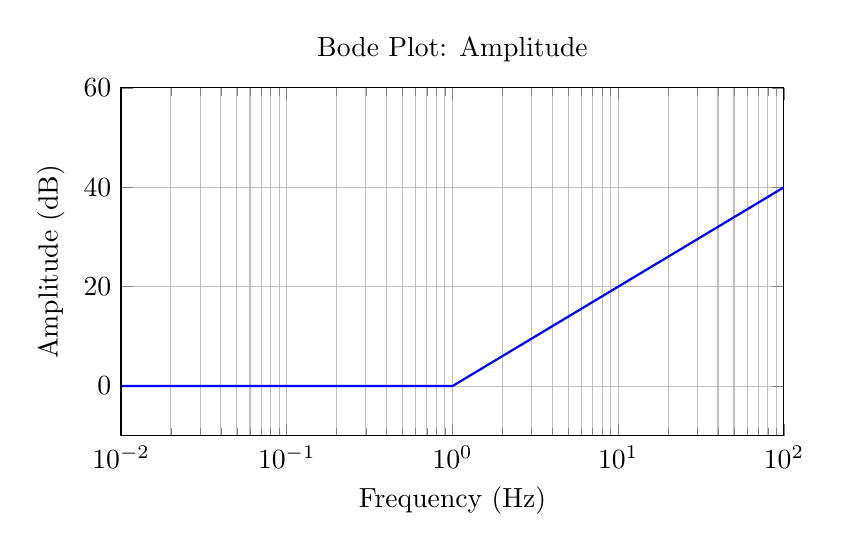
\begin{tikzpicture}
                \begin{semilogxaxis}[
                    title={Bode Plot: Amplitude},
                    xlabel={Frequency (Hz)},
                    ylabel={Amplitude (dB)},
                    grid=both,
                    xmin=1e-2, xmax=1e2,
                    ymin=-10, ymax=60,
                    width=10cm,
                    height=6cm
                ]
                    % Amplitude plot
                    \addplot[
                        thick,
                        blue
                    ]
                    coordinates {
                        (1e-2, 0) (1e-1, 0) (1, 0) (10, 20) (100, 40)
                    };
                \end{semilogxaxis}
            \end{tikzpicture}
            \end{figure}
            \begin{figure}[H]
                \centering
                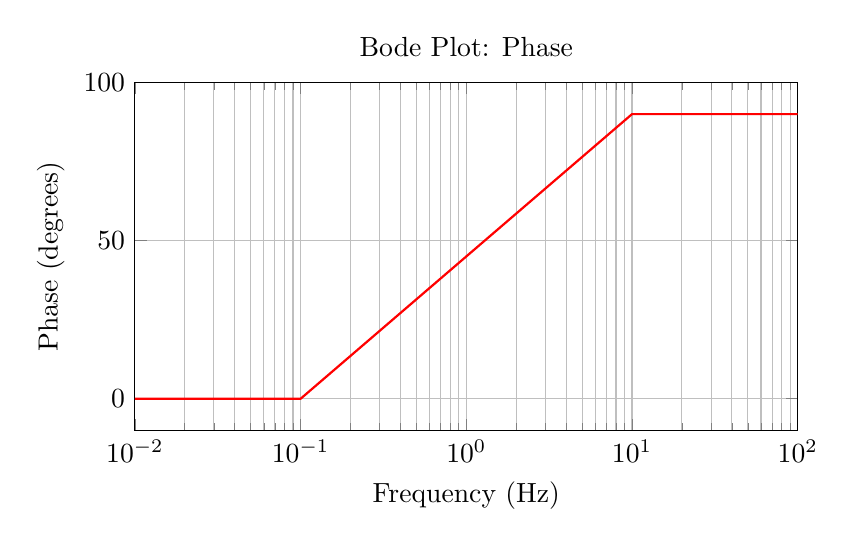
\begin{tikzpicture}
                    \begin{semilogxaxis}[
                        title={Bode Plot: Phase},
                        xlabel={Frequency (Hz)},
                        ylabel={Phase (degrees)},
                        grid=both,
                        xmin=1e-2, xmax=1e2,
                        ymin=-10, ymax=100,
                        width=10cm,
                        height=6cm
                    ]
                        % Phase plot
                        \addplot[
                            thick,
                            red
                        ]
                        coordinates {
                            (1e-2, 0) (1e-1, 0) (1, 45) (10, 90) (100, 90)
                        };
                    \end{semilogxaxis}
                \end{tikzpicture}                
            \end{figure}
            \item $s^2$ dove $\mu = 2$:
            \[A = 20\mu\log(\mu) = 40db/dec\]
            \[\phi = \mu 90\degree = 180\degree\]
            \begin{figure}[H]
                % Amplitude plot
                \centering
                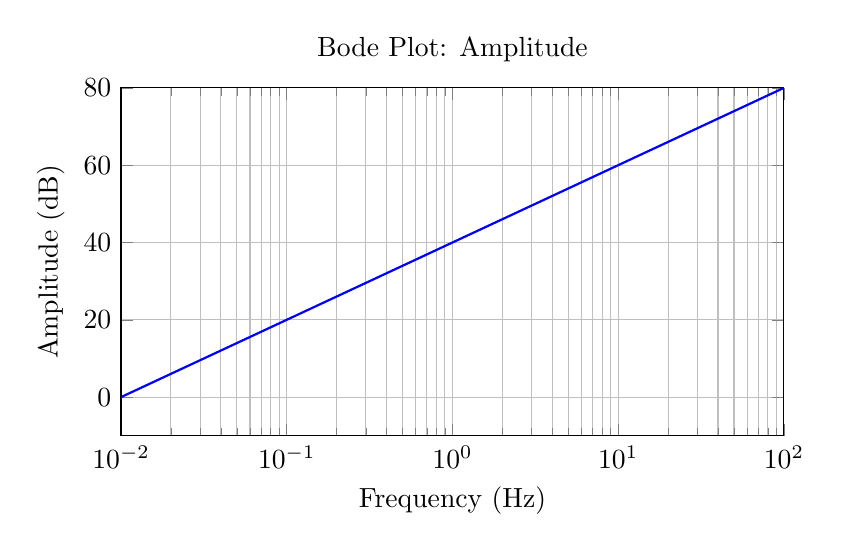
\begin{tikzpicture}
                    \begin{semilogxaxis}[
                        title={Bode Plot: Amplitude},
                        xlabel={Frequency (Hz)},
                        ylabel={Amplitude (dB)},
                        grid=both,
                        xmin=1e-2, xmax=1e2,
                        ymin=-10, ymax=80,
                        width=10cm,
                        height=6cm
                    ]
                        % Amplitude plot
                        \addplot[
                            thick,
                            blue
                        ]
                        coordinates {
                            (1e-2, 0) (1e-1, 20) (1, 40) (10, 60) (100, 80)
                        };
                    \end{semilogxaxis}
                \end{tikzpicture}
            \end{figure}
            \begin{figure}[H]
                \centering
                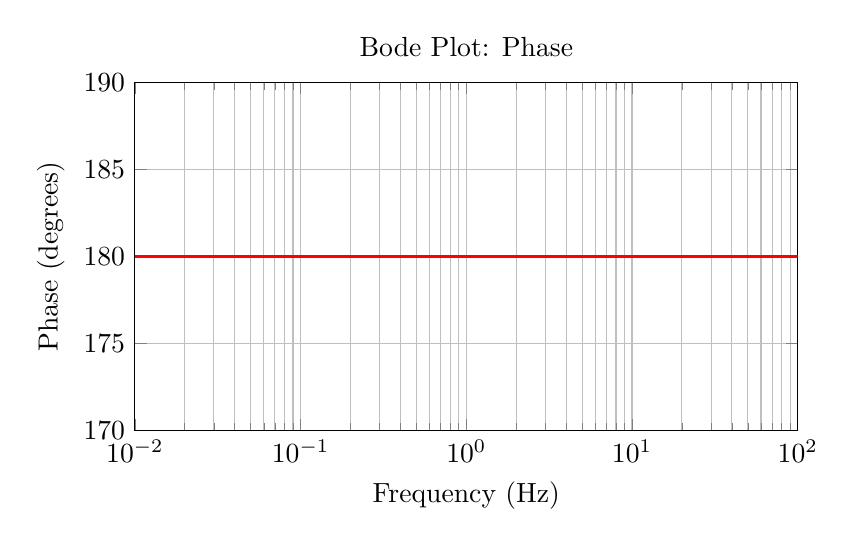
\begin{tikzpicture}
                    \begin{semilogxaxis}[
                        title={Bode Plot: Phase},
                        xlabel={Frequency (Hz)},
                        ylabel={Phase (degrees)},
                        grid=both,
                        xmin=1e-2, xmax=1e2,
                        ymin=170, ymax=190,
                        width=10cm,
                        height=6cm
                    ]
                        % Phase plot
                        \addplot[
                            thick,
                            red
                        ]
                        coordinates {
                            (1e-2, 180) (1e-1, 180) (1, 180) (10, 180) (100, 180)
                        };
                    \end{semilogxaxis}
                \end{tikzpicture}
            \end{figure}
            \item $\left(1 + \frac{3}{16}s + \frac{s^2}{16}\right)$ dove $\mu = 1$ e $\omega_n = \sqrt{16} = 4$ e $\frac{2\zeta}{\omega_n} = \frac{3}{16} \Longrightarrow \zeta = \frac{3}{8}$:
            \[A = 40\mu\log_{10}\left(\frac{\omega}{\omega_n}\right) = 40db/decade\]
            quindi prima di $4$, $A = 0$ e dopo $4$, $A = 40db/decade$. Ora calciamo $\omega_r$ e $M_r$: \dots
            Per la fase
            \[\phi = 180\mu sgn(\zeta) = 180\degree\]
            Dopo $\omega_n$ la fase è di $180\degree$ mentre prima la fase rimane a $\phi = 0\degree$
            \begin{figure}[H]
                \centering
                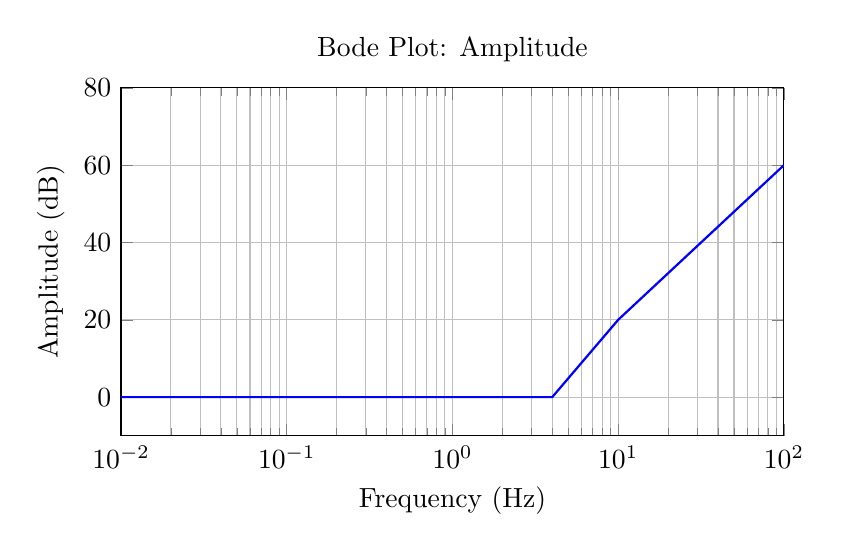
\begin{tikzpicture}
                    \begin{semilogxaxis}[
                        title={Bode Plot: Amplitude},
                        xlabel={Frequency (Hz)},
                        ylabel={Amplitude (dB)},
                        grid=both,
                        xmin=1e-2, xmax=1e2,
                        ymin=-10, ymax=80,
                        width=10cm,
                        height=6cm
                    ]
                        % Amplitude plot
                        \addplot[
                            thick,
                            blue
                        ]
                        coordinates {
                            (1e-2, 0) (1, 0) (4, 0) (10, 20) (100, 60)
                        };
                    \end{semilogxaxis}
                \end{tikzpicture}
            \end{figure}
            \begin{figure}[H]
                \centering
                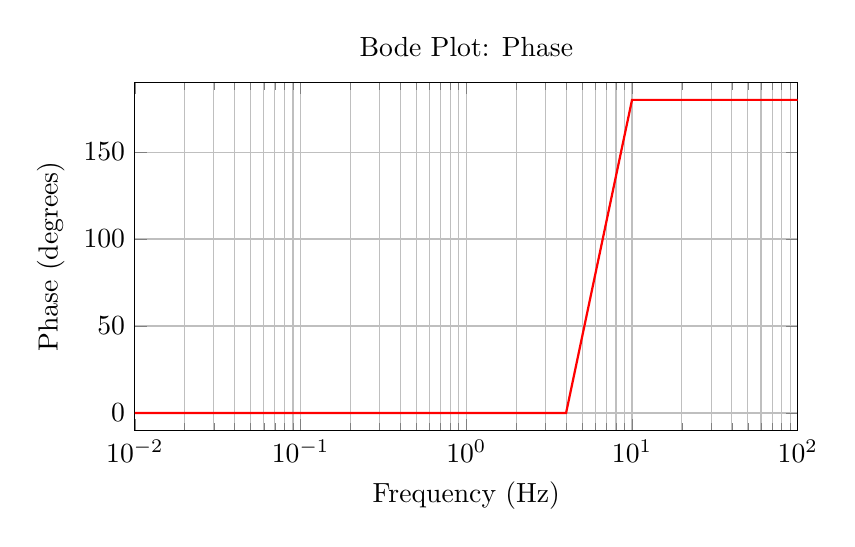
\begin{tikzpicture}
                    \begin{semilogxaxis}[
                        title={Bode Plot: Phase},
                        xlabel={Frequency (Hz)},
                        ylabel={Phase (degrees)},
                        grid=both,
                        xmin=1e-2, xmax=1e2,
                        ymin=-10, ymax=190,
                        width=10cm,
                        height=6cm
                    ]
                        % Phase plot
                        \addplot[
                            thick,
                            red
                        ]
                        coordinates {
                            (1e-2, 0) (1, 0) (4, 0) (10, 180) (100, 180)
                        };
                    \end{semilogxaxis}
                \end{tikzpicture}
            \end{figure}
        \end{itemize}
    \end{enumerate}
\end{examplebox}

\subsection{Diagrammi di Bode Totale}

\pagebreak

\section{Trasformata di Fourier}

Fourier ha scoperto che qualsiasi segnale periodico (o aperiodico) può essere scomposto in una somma di sinusoidi.
Con Fourier si riesce a rappresentare con somma di frequenze che non sono necessariamente armoniche.
Le trasformate di Fourier vengono usate in molti campi come la comunicazione, analisi del suono, modulazione o demoloduzione dei segnali, meccanica, cambiamento climatico, ecc.


\begin{figure}[H]
    \centering
    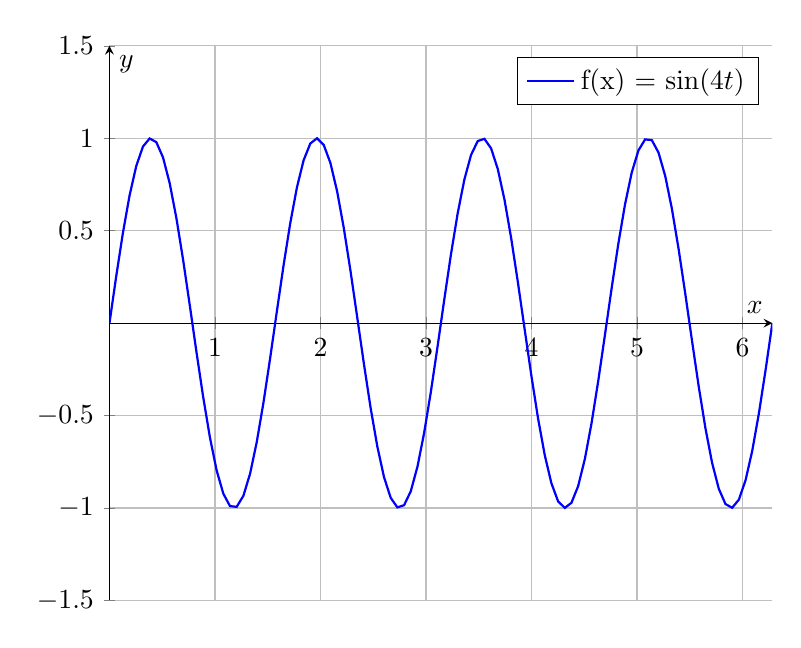
\begin{tikzpicture}
        \begin{axis}[
            axis lines = middle, 
            xlabel={$x$}, ylabel={$y$},
            domain=0:2*pi, 
            grid=both,
            xmin=0, xmax=2*pi, ymin=-1.5, ymax=1.5
        ]
            \addplot[blue, thick, samples=100] {sin(4*deg(x))};
            \legend{f(x) = $\sin(4t)$}
        \end{axis}
        \end{tikzpicture}
\end{figure}

\begin{figure}[H]
    \centering
    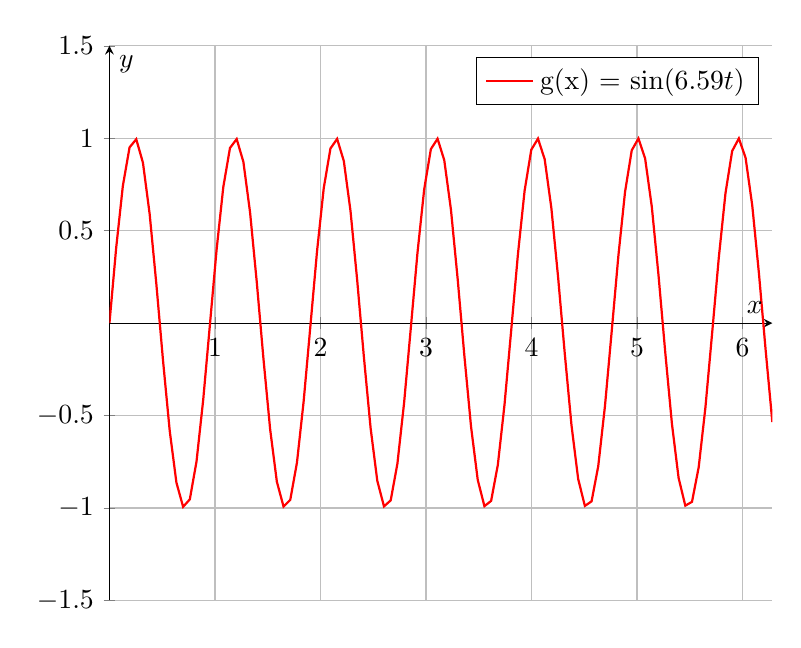
\begin{tikzpicture}
        \begin{axis}[
            axis lines = middle, 
            xlabel={$x$}, ylabel={$y$},
            domain=0:2*pi, 
            grid=both,
            xmin=0, xmax=2*pi, ymin=-1.5, ymax=1.5
        ]
            \addplot[red, thick, samples=100] {sin(6.59*deg(x))};
            \legend{g(x) = $\sin(6.59t)$}
        \end{axis}
        \end{tikzpicture}
\end{figure}

\begin{figure}[H]
    \centering
    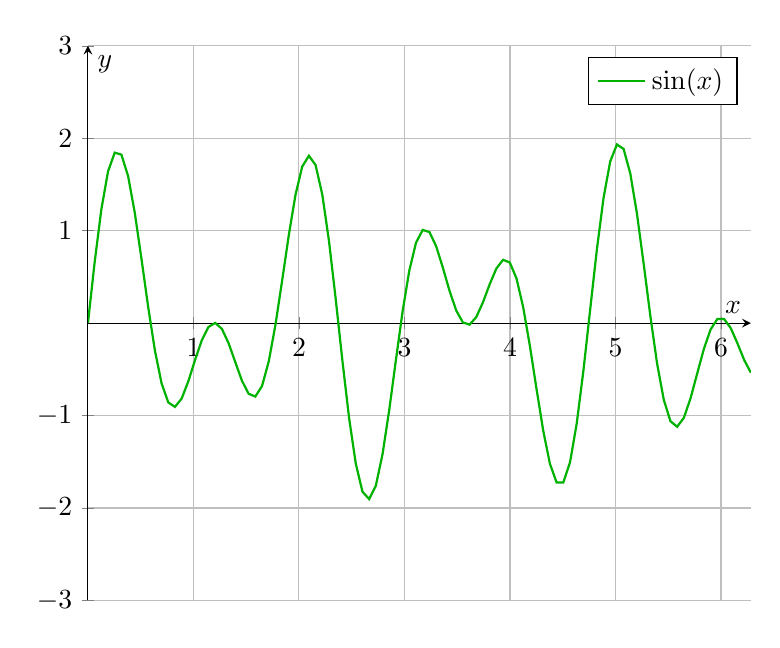
\begin{tikzpicture}
        \begin{axis}[
            axis lines = middle, 
            xlabel={$x$}, ylabel={$y$},
            domain=0:2*pi, 
            grid=both,
            xmin=0, xmax=2*pi, ymin=-3, ymax=3
        ]
            \addplot[green!70!black, thick, samples=100] {sin(6.59*deg(x)) + sin(4*deg(x))};
            \legend{$\sin(x)$}
        \end{axis}
        \end{tikzpicture}
        \caption{Somma di f(x) e g(x)}
\end{figure}
Ci sono diversi tipi di onde che psosono essere sommate per creare un segnale complesso.
Come per esempio le onde quadre, triangolari, ecc. 

\subsection{Winding Frequency e la quasi-trasformata di Fourier}

Calcoliamo il centro di massa come la media dei punti sul grafico:

\[cdm = \frac{1}{n} \sum_{k=1}^n g(t_k)e^{-2\pi f_0t}\]
per cui possiamo trovare il limite:
\[\lim_{n \rightarrow \infty} \frac{1}{n} \sum_{k=1}^n g(t_k)e^{-2\pi f_0t} = \underbrace{\frac{1}{t_2 - t_1}\bigg|_{t_1}^{t_2} -g(t_k i f_0t) dt}_{\text{Quasi TdF}}\]
Quindi:
\begin{align*}
    TdF &= \int_{-\infty}^{+\infty} g(t)e^{-2\pi i f_0t} dt\\
\end{align*}
Proprio come la trasformata di LaPlace ci è utile spostarsi nel dominio delle frequenze da quello del tempo.


\[\underbrace{e^{j\omega_k t}}_{input} \rightarrow LTI \rightarrow \underbrace{H(\omega_k)}_{Transf. Fun}e^{j\omega_k t}\]
Questo è il principio di sovrapposizione. Il principio di sovrapposizione dice 
che se un sistema è lineare e invariante nel tempo, allora la risposta a una somma di segnali è la somma delle risposte ai singoli segnali.

\subsection{Segnali periodici e aperiodici}

Se abbiamo un segnale \textbf{periodico} possiamo scomporlo in una somma (finita) di funzioni elementari tramite la serie di Fourier.
Invece per un segnale \textbf{aperiodico}, quindi privo di periodicità, andremo ad utilizzare la trasformata di Fourier.
Mentre nella serie di Fourier le funzioni sono strettamente \textit{collegate} a livello armonico, nella trasformata di Fourier le funzioni sono \textit{indipendenti}.

\subsection{Serie di Fourier}

Prendiamo come un segnale periodico $x(t)$ con periodo $t_0$:
\[x(t) = x(t + t_0)\]
\[\omega_0 = \frac{2\pi}{t_0} = 2\pi f_0 \leftarrow \text{ funzione fondamentale}\]
Se passiamo alla rappresentazione complessa:
\[e^{j\omega_0t} \rightarrow t_0 = \frac{2\pi}{\omega_0}\]
\[\phi_k(t) = e^{jk\omega_0 t} \rightarrow t_0 = \frac{2\pi}{k\omega_0}\]
Questa è una famiglia di funzioni che sono armonicamente collegate perché 
come si può vedere i loro periodi sono soltanto multipli interi del periodo fondamentale.
Riscriviamo $x(t)$ come combinazione lineare di $\phi_k$:
\[x(t) = \sum_{k = -\infty}^{+\infty} a_k e^{jk\omega_0 t}\]
Dove $a_k$ sono i coefficienti della serie di Fourier.
\begin{theorem}
    Si può riscrevere un segnale periodico in somme di sengnali elementari.
    \[x(t) = \sum_{k = -\infty}^{+\infty} a_k e^{jk\omega_0 t}\]
    dove $a_k$ sono i coefficienti della serie di Fourier, $k$ è l'indice di armonica e 
    $\omega_0$ è la frequenza fondamentale. Viene anche chiamata \textbf{equazione di sintesi}.
\end{theorem}
I coefficienti $a_k$ si possono calcolare come:
\begin{align*}
    a_k &= A_k e^{j\theta k}\\
    &= B_k + j C_k
\end{align*}
Quindi modificando trigonometricamente:
\begin{align*}
 e^{jk\omega_0 t} &= \cos(k\omega_0 t) + j\sin(k\omega_0 t)\\
 x(t) &= a_0 + 2\sum_{k = 1}^{+\infty} A_k \cos(k\omega_0 t + \phi_k)\\
 \text{oppure } &=   a_0 + 2\sum_{k = 1}^{+\infty} \left[B_k\cos(k\omega_0 t) - iC_k\sin(k\omega_t)\right]\\
\end{align*}
Come facciamo a calcolare i coefficienti $a_k$?
\begin{align*}
    a_k &= \int_{t_0} e^{-jk\omega_0 t} dt = \begin{cases}
        t_0 & \text{ se } k = 0\\
        0 & \text{ se } k \neq 0
    \end{cases}\\
    &= \int_{t_0} \cos(k\omega_0 t) dt - \int_{t_0} \sin(k\omega_0 t) dt\\
\end{align*}
Si fa quindi l'integrale sul periodo di $x(t)$.
\begin{align*}
    \int_{t_0} x(t) e^{-jN\omega_0 t} dt &= \int_{t_0} \sum_{k = -\infty}^{+\infty} a_k e^{jk\omega_0 t} e^{-jN\omega_0 t} dt\\
    &= \sum_{k = -\infty}^{+\infty} a_k  \underbrace{\int_{t_0} e^{-j(k - N)\omega_0 t} dt}_{\begin{cases}
        t_0 & \text{ se } k = N\\
        0 & \text{ se } k \neq N
    \end{cases}}
\end{align*}
\begin{theorem}
    L'equazione di analisi di Fourier è:
    \[a_k = \frac{1}{t_0} \int_{t_0} x(t) e^{-jk\omega_0 t} dt\]
\end{theorem}


\subsubsection{Segnali simmetrici e asimmetrici}
\begin{itemize}
  \item \textbf{Segnale periodico non-simmetrico}
    \begin{figure}[H]
      \centering
      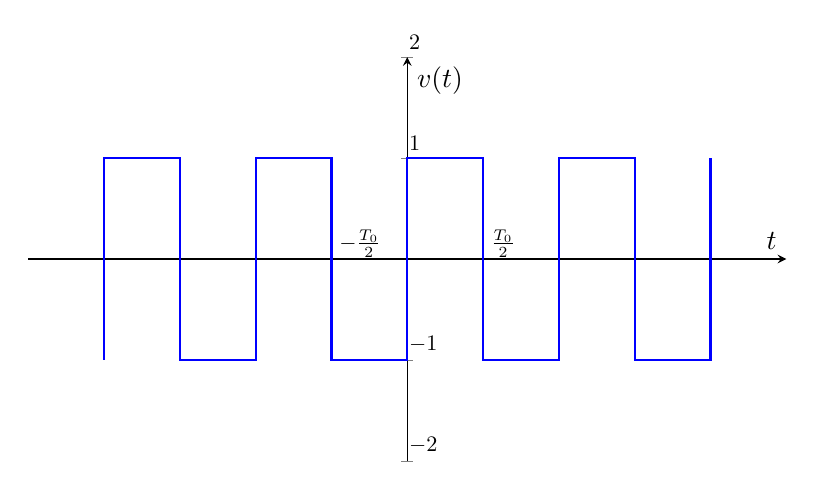
\begin{tikzpicture}
        \begin{axis}[
          scale=1.5,
          width=8cm,
          height=5cm,
          ylabel = \( v(t) \),
          xlabel = \( t \),
          ymin=-2, ymax=2,
          xmin=-5, xmax=5,
          xtick = {-1,1},
          xticklabels = {$-\frac{T_0}{2}$, $\frac{T_0}{2}$},
          yticklabel style = {anchor=south west, scale=0.8},
          xticklabel style = {anchor=south west, scale=0.8},
          axis lines = center
          ]
          \addplot[blue, thick] coordinates {
            (-4,-1) (-4,1)
            (-3,1) (-3,-1)
            (-2,-1) (-2,1)
            (-1,1) (-1,-1)
            (0,-1) (0,1)
            (1,1) (1,-1)
            (2,-1) (2,1)
            (3,1) (3,-1)
            (4,-1) (4,1)
          };
        \end{axis}
      \end{tikzpicture}
      \caption{Segnale periodico non-simmetrico}
    \end{figure}
    \[
      a_k = \frac{1}{T_0} \int_{\frac{-T_0}{2}}^{0} \stackrel{v(t)}{(-1)} \cdot e^{-j k \omega_0 t} \, dt +
      \frac{1}{T_0} \int_{0}^{\frac{T_0}{2}} \stackrel{v(t)}{1} \cdot e^{-j k \omega_0 t} \, dt
    \] 
    \[
      \stackrel{\vdots}{\downarrow}
    \] 
    \[
      a_k = \frac{1}{j \pi k} \left[ 1 - (-1)^k \right] \quad k \neq 0
    \] 

    \vspace{1em}
    \noindent
    Il grafico dei coefficienti è il seguente:
    \begin{figure}[H]
      \centering
      \begin{tikzpicture}
        \begin{axis}[
          width = 1\textwidth,
          height = 0.6\textwidth,
          ylabel = \( j \pi a_k \),
          xlabel = \( \omega \),
          ymin=-3, ymax=3,
          xmin=-6, xmax=6,
          ytick=\empty,
          xtick = {-5,-4,...,5},
          xticklabel style = {scale=0.8},
          axis lines = center
          ]
          \addplot[blue, mark=*, mark size=1.5pt] coordinates {
              (-5,-2/5) (-4,0) (-3,-2/3) (-2,0) (-1,-2) (0,0)
              (1,2) (2,0) (3,2/3) (4,0) (5,2/5)
          };
          
          \node[below, scale=0.8] at (axis cs:-5,-2/5) {\( -\frac{2}{5} \)};
          \node[below, scale=0.8] at (axis cs:-3,-2/3) {\( -\frac{2}{3} \)};
          \node[below, scale=0.8] at (axis cs:-1,-2) {\( -2 \)};
          \node[above, scale=0.8] at (axis cs:1,2) {\( 2 \)};
          \node[above, scale=0.8] at (axis cs:3,2/3) {\( \frac{2}{3} \)};
          \node[above, scale=0.8] at (axis cs:5,2/5) {\( \frac{2}{5} \)};
        \end{axis}
      \end{tikzpicture}
      \caption{Coefficienti \( a_k \) per segnale non-simmetrico}
    \end{figure}

    \begin{itemize}
      \item Armoniche dispari
      \item \( a_k \) immaginari
      \item \( a_k = -a_{-k}\) antisimmetrico
    \end{itemize}
    Siccome tutti i coefficienti sono immaginari si ha una serie di seni e si può
    riscrivere come:
    \[
      v(t) = a_0 + \sum_{k=1}^{+\infty} \underbrace{2j}_{\text{Per avere termini reali}} \cdot a_k \sim(k \omega_0 t)
    \] 

  \item \textbf{Segnale periodico simmetrico}
    \begin{figure}[H]
      \centering
      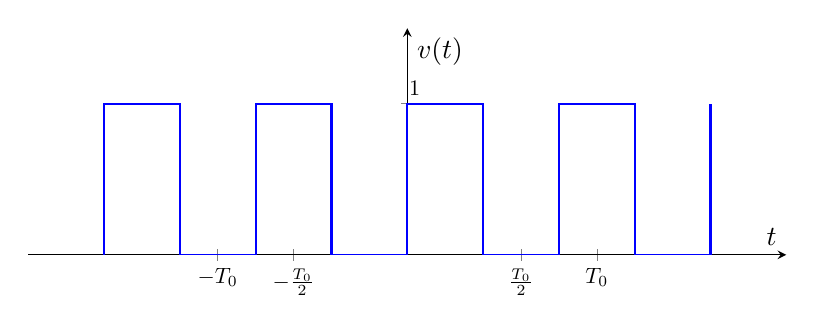
\begin{tikzpicture}
        \begin{axis}[
          scale=1.5,
          width=8cm,
          height=3.5cm,
          ylabel = \( v(t) \),
          xlabel = \( t \),
          ymin=0, ymax=1.5,
          xmin=-5, xmax=5,
          xtick = {-2.5,-1.5,1.5,2.5},
          ytick = {1},
          xticklabels = {$-T_0$, $-\frac{T_0}{2}$, $\frac{T_0}{2}$, $T_0$},
          yticklabel style = {anchor=south west, scale=0.8},
          xticklabel style = {anchor=north, scale=0.8},
          axis lines = center
          ]
          \addplot[blue, thick] coordinates {
            (-4,0) (-4,1)
            (-3,1) (-3,0)
            (-2,0) (-2,1)
            (-1,1) (-1,0)
            (0,0) (0,1)
            (1,1) (1,0)
            (2,0) (2,1)
            (3,1) (3,0)
            (4,0) (4,1)
          };
        \end{axis}
      \end{tikzpicture}
      \caption{Segnale periodico simmetrico}
    \end{figure}
    \[
    a_k = \begin{cases}
      \frac{1}{2} & k = 0\\
      \frac{\sin\left( \frac{\pi k}{2} \right)}{\pi k} & k \neq 0
    \end{cases}
    \] 

    \vspace{1em}
    \noindent
    Il grafico dei coefficienti è il seguente:
    \begin{figure}[H]
      \centering
      \begin{tikzpicture}
        \begin{axis}[
          clip=false,
          width = 1\textwidth,
          height = 0.6\textwidth,
          ylabel = \( j \pi a_k \),
          xlabel = \( \omega \),
          ymin=-1/2, ymax=2,
          xmin=-5.5, xmax=5.5,
          ytick=\empty,
          xtick = {-5,-4,...,5},
          xticklabel style = {scale=0.8},
          axis lines = center
          ]
          \addplot[blue, mark=*, mark size=1.5pt] coordinates {
              (-5,1/5) (-4,0) (-3,-1/3) (-2,0) (-1,1) (0,1/2)
              (1,1) (2,0) (3,-1/3) (4,0) (5,1/5)
          };
          
          \node[above right, scale=0.8] at (axis cs:0,1/2) {\( \frac{1}{2} \)};
          \node[above, scale=0.8] at (axis cs:1,1) {\( 1 \)};
          \node[below, scale=0.8] at (axis cs:3,-1/3) {\( -\frac{1}{3} \)};
          \node[above, scale=0.8] at (axis cs:5,1/5) {\( \frac{1}{5} \)};
        \end{axis}
      \end{tikzpicture}
      \caption{Coefficienti \( a_k \) per segnale simmetrico}
    \end{figure}

    \begin{itemize}
      \item Armoniche dispari
      \item \( a_k \) è reale
      \item \( a_k = a_{-k} \) simmetrico
    \end{itemize}
    Siccome tutti i coefficienti sono reali si ha una serie di coseni e si può riscrivere
    come:
    \[
      v(t) = a_0 + \sum_{k=1}^{+\infty} 2 \cdot a_k \cos(k \omega_0 t)
    \] 
\end{itemize}

\subsubsection{Serie di Fourier troncata}
Serve per limitare la sommatoria a \( N \) termini.

\vspace{1em}
\noindent
Sia \( N \in \mathbb{Z} \) 
\[
  \underbrace{v_N(t)}_{\text{\( v(t) \) rappresentato con \( N \) componenti}} =
  \sum_{k=-N}^{N} \tilde{a}_k \cdot e^{j k \omega_0 t} \quad a_k \in \mathbb{C}, \quad \omega_0,t \in \mathbb{R},
  \quad k \in \mathbb{Z}
\] 
Calcoliamo l'errore quadratico medio (MSE, Mean Square Error) che è la misura
dell'errore di approssimazione
\[
  MSE\left(v(t),v_N(t)\right) := \frac{1}{T_0} \int_{T_0} |v(t) - v_N(t)|^2 \, dt
\] 
misura l'energia della differenza di due segnali.
\[
  \tilde{a}_k = a_k = \lim_{N \to \infty} MSE\left(v(t),v_N(t)\right) = 0
\] 
\begin{examplebox}{Definizione}
  \textbf{Fenomeno di Gibs}: Aumentando il numero di armoniche si ha un aumento
  di armoniche ad alta frequenza nei punti di discontinuità.
  \begin{figure}[H]
    \centering
    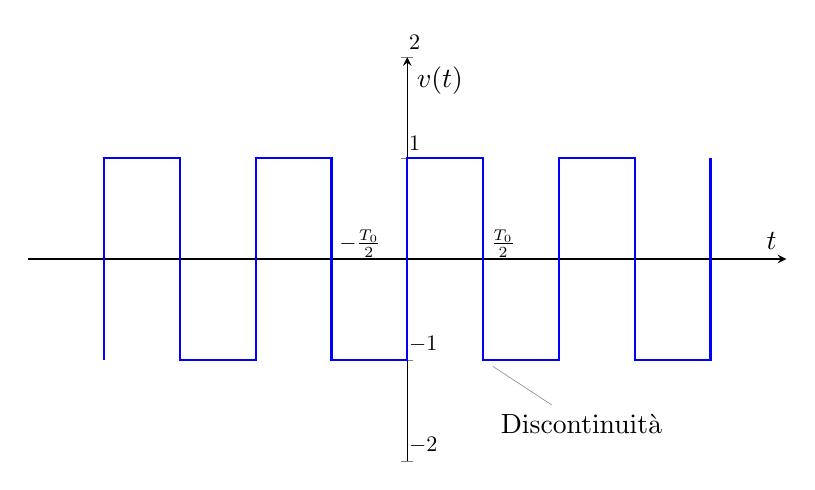
\begin{tikzpicture}
      \begin{axis}[
        scale=1.5,
        width=8cm,
        height=5cm,
        ylabel = \( v(t) \),
        xlabel = \( t \),
        ymin=-2, ymax=2,
        xmin=-5, xmax=5,
        xtick = {-1,1},
        xticklabels = {$-\frac{T_0}{2}$, $\frac{T_0}{2}$},
        yticklabel style = {anchor=south west, scale=0.8},
        xticklabel style = {anchor=south west, scale=0.8},
        axis lines = center
        ]
        \addplot[blue, thick] coordinates {
            (-4,-1) (-4,1)
            (-3,1) (-3,-1)
            (-2,-1) (-2,1)
            (-1,1) (-1,-1)
            (0,-1) (0,1)
            (1,1) (1,-1)
            (2,-1) (2,1)
            (3,1) (3,-1)
            (4,-1) (4,1)
          };

        \node[font=\tiny, pin=280:{Discontinuità}] at (axis cs:1,-1) {};
      \end{axis}
    \end{tikzpicture}
    \caption{Discontinuità}
  \end{figure}
  \[
  T = 2 \pi \quad \text{Non simmetrico}
  \] 
  \[
  t = k \pi 
  \]
  \[
    \begin{aligned}
      v(t) &= a_0 + \sum_{k=-\infty}^{+\infty} B_k \sin(k \omega_0 t)\\
      a_k  &= \frac{1}{2 \pi } \int_{0}^{2 \pi} v(t) e^{-j k \omega_0 t} \, dt \\
           &= \frac{-i}{2 \pi k} \left( 2 - 2 e^{-j \pi t} \right) 
    \end{aligned}
  \] 
  \[
  a_k = \begin{cases}
    \frac{-2 j}{k \pi } & k \text{ è dispari}\\
    0 & \text{altrimenti}
  \end{cases}
  \] 
\end{examplebox}

\subsection{Dalla serie di Fourier alla trasformata di Fourier}
Se si ha un segnale non periodico che va da \( \left[ -T_1, T_1 \right] \):
\begin{figure}[H]
  \centering
  \begin{tikzpicture}
    \def\Tone{2}
    \begin{axis}[
      height = 0.4\textwidth,
      ylabel = $v(t)$,
      xlabel = $t$,
      xmin=-\Tone*2, xmax=\Tone*2,
      ymin= 0, ymax = 3,
      ytick = \empty,
      xtick = {-\Tone, \Tone},
      xticklabels = {$-T_1$, $T_1$},
      axis lines = middle,
      declare function ={ f(\x) = sin(deg(\x))/2 + 1.5; },
    ]
      \addplot[blue,thick,domain=-\Tone:\Tone,samples=100]{f(x)};
      \draw[dashed] (axis cs:-\Tone,0) -- (axis cs:-\Tone,{f(-\Tone)});
      \draw[dashed] (axis cs:\Tone,0) -- (axis cs:\Tone,{f(\Tone)});
    \end{axis}
  \end{tikzpicture}
  \caption{Segnale non periodico}
\end{figure}

\[
  \underbrace{\tilde{v}(t)}_{\text{Periodico}} = \underbrace{v(t)}_{\text{Non periodico}}
\] 
\[
|t| < \frac{T_0}{2}
\] 
Se \( T_0 \to \infty \) si ha che \( \tilde{v}(t) \to v(t) \). Cioè si prende un segnale
periodico e si fa tendere il periodo a infinito facendolo sembrare non periodico.
Questo passaggio si può fare anche al contrario, cioè prendere un segnale non periodico
e farlo diventare periodico.
\begin{itemize}
  \item Usiamo la serie di Fourier per rappresentare \( \tilde{v}(t) \) 
  \item Facciamo tendere \( T_0 \) a infinito \( T_0 \to \infty \) per rappresentare \( v(t) \)
\end{itemize}

\begin{examplebox}{Esempio}
  Partiamo da un segnale non periodico e lo replichiamo nel tempo con periodo \( T_0 \) 
  \begin{figure}[H]
    \centering
    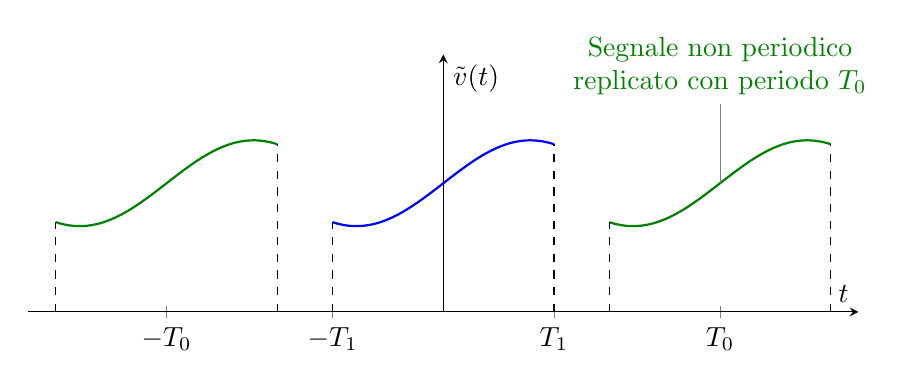
\begin{tikzpicture}
      \def\Tone{2}
      \def\Tzero{2.5*\Tone}
      \begin{axis}[
        clip=false,
        width = 1\textwidth,
        height = 0.4\textwidth,
        ylabel = $\tilde{v}(t)$,
        xlabel = $t$,
        xmin=-\Tzero*1.5, xmax=\Tzero*1.5,
        ymin= 0, ymax = 3,
        ytick = \empty,
        xtick = {-\Tzero, -\Tone, \Tone, \Tzero},
        xticklabels = {$-T_0$, $-T_1$, $T_1$, $T_0$},
        axis lines = middle,
        declare function ={ f(\x) = sin(deg(\x))/2 + 1.5; },
        ]
        \addplot[blue,thick,domain=-\Tone:\Tone,samples=100]{f(x)};
        \draw[dashed] (axis cs:-\Tone,0) -- (axis cs:-\Tone,{f(-\Tone)});
        \draw[dashed] (axis cs:\Tone,0) -- (axis cs:\Tone,{f(\Tone)});

        \addplot[green!50!black,thick,domain=-\Tone -\Tzero:\Tone - \Tzero,samples=100]{f(x + \Tzero)};
        \draw[dashed] (axis cs:-\Tone-\Tzero,0) -- (axis cs:-\Tone-\Tzero,{f(-\Tone)});
        \draw[dashed] (axis cs:\Tone-\Tzero,0) -- (axis cs:\Tone-\Tzero,{f(\Tone)});


        \addplot[green!50!black,thick,domain=-\Tone +\Tzero:\Tone + \Tzero,samples=100]{f(x - \Tzero)};
        \draw[dashed] (axis cs:-\Tone+\Tzero,0) -- (axis cs:-\Tone+\Tzero,{f(-\Tone)});
        \draw[dashed] (axis cs:\Tone+\Tzero,0) -- (axis cs:\Tone+\Tzero,{f(\Tone)});

        \node[coordinate, pin={[green!50!black,align=center,pin distance=1cm]above:Segnale non periodico\\replicato con periodo $T_0$}] at (axis cs:\Tzero,{f(0)}) {};
      \end{axis}
    \end{tikzpicture}
    \caption{Segnale non periodico replicato}
  \end{figure}
  \[
    \tilde{v}(t) = v(t) \quad |t| < \frac{T_0}{2}
  \] 
  Applichiamo la serie di Fourier su \( \tilde{v}(t) \):
  \[
    \tilde{v}(t) = \sum_{k=-\infty}^{+\infty} \tilde{a}_k \cdot e^{j k \omega_0 t}
  \] 
  \[
    \omega_0 = \frac{2 \pi}{T_0} = 2 \pi f_0
  \] 
  \[
    \begin{aligned}
      a_k &= \frac{1}{T_0} \int_{-\frac{T_0}{2}}^{\frac{T_0}{2}} \tilde{v}(t) e^{-j k \omega_0 t} \, dt\\
          &= \frac{1}{T_0} \int_{-\infty}^{+\infty} v(t) e^{-j k \omega_0 t} \, dt
    \end{aligned}
  \] 
  Rappresentiamo \( k \omega_0 \) con una funzione \( V(\omega) \) 
  \[
    V(\omega) := \int_{-\infty}^{+\infty} v(t) e^{-j \omega t} \, dt \quad \to \quad
    T_0 a_k = V(\omega) \Big|_{\omega = k \omega_0}
  \] 
  \( V(\omega) \) è l'\textbf{inviluppo} di \( T_0 a_k \):
  \begin{figure}[H]
    \centering
    \begin{tikzpicture}
      \begin{axis}[
        width = 1\textwidth,
        height = 0.6\textwidth,
        ylabel = \( j \pi a_k \),
        xlabel = \( \omega \),
        ymin=-3, ymax=3,
        xmin=-6, xmax=6,
        ytick=\empty,
        xtick={1,...,5},
        xticklabel style = {scale=0.8},
        axis lines = center
        ]
        \addplot[blue, mark=*, mark size=1.5pt] coordinates {
            (-5,-2/5) (-4,0) (-3,-2/3) (-2,0) (-1,-2) (0,0)
            (1,2) (2,0) (3,2/3) (4,0) (5,2/5)
          };

        \node[pin={[]right:$T_0 a_k$}] at (axis cs: 1, 2) {};
        \node[pin={[blue]above:$V(w)$}] at (axis cs: 4.5, 0.1) {};
      \end{axis}
    \end{tikzpicture}
    \caption{Inviluppo di \( T_0 a_k \)}
  \end{figure}

  \vspace{1em}
  \noindent
  \[
    \begin{aligned}
      \tilde{v}(t) &= \sum_{k=-\infty}^{+\infty} a_k \cdot e^{j k \omega_0 t}\\
                   &= \sum_{k=-\infty}^{+\infty} \frac{1}{T_0} V(k \omega_0) \cdot e^{j k \omega_0 t}\\
    \end{aligned}
  \] 
  \[
  \downarrow
  \] 
  \[
    \tilde{v}(t) = \frac{1}{2 \pi } \sum_{k=-\infty}^{+\infty} V(k \omega_0) \cdot e^{j k \omega_0 t} \omega_0
  \] 
  Se \( T_0 \to \infty \) otteniamo che:
  \begin{itemize}
    \item \( \omega_0 \to 0 \) 
    \item \( \tilde{v}(t) \to v(t) \) 
    \item \( \omega_0 \to d \omega \) 
    \item \( \sum \to \int \) 
  \end{itemize}
  Con queste premesse possiamo riscrivere la funzione come:
  \[
    \tilde{v}(t) = \frac{1}{2 \pi } \sum_{-\infty}^{+\infty} V(k \omega_0) \cdot e^{j k \omega_0 t} \omega_0
  \] 
  \[
  \downarrow
  \] 
  \[
    v(t) = \frac{1}{2 \pi } \int_{-\infty}^{+\infty} V(\omega) \cdot e^{j \omega t} \, d\omega
  \] 
  È la trasformata di Fourier inversa.

  \vspace{1em}
  \noindent
  \[
    V(\omega) = \int_{-\infty}^{+\infty} v(t) \cdot e^{-j \omega t} \, dt
  \] 
  È la trasformata di Fourier.
\end{examplebox}

\begin{definition}
  \[
    v(t) = \frac{1}{2 \pi } \int_{-\infty}^{+\infty} V(\omega) \cdot e^{j \omega t} \, d\omega
  \] 
  È l'\textbf{equazione di sintesi per un segnale non periodico} che equivale alla
  trasformata \textbf{inversa} di Fourier.

  \vspace{1em}
  \noindent
  \[
    V(\omega) = \int_{-\infty}^{+\infty} v(t) \cdot e^{-j \omega t} \, dt
  \] 
  È l'\textbf{equazione di analisi per un segnale non periodico} che equivale alla
  \textbf{trasformata di Fourier}.
\end{definition}

\begin{examplebox}{Esempio}
  Prendiamo ad esempio un segnale non periodico:
  \[
    v(t) = e^{-at}
  \] 
  Calcoliamo la trasformata di Fourier:
  \[
    \begin{aligned}
      V(\omega) &= \int_{-\infty}^{+\infty} v(t) \cdot e^{-j \omega t} \, dt\\
                &= \int_{-\infty}^{+\infty} e^{-t (a+j \omega)} \, dt\\
                &= \frac{-1}{a + j \omega} \cdot e^{-(a+j \omega)t} \Big|_{\infty}^{0}\\
                &= \frac{1}{a + j \omega}
    \end{aligned}
  \] 

  \vspace{1em}
  \noindent
  Con Laplace sarebbe stato:
  \[
    e^{\lambda t} = \frac{1}{s - \lambda}
  \] 
  \[
  \downarrow
  \] 
  \[
    e^{-at} = \frac{1}{s + a} = \frac{1}{a + j \omega}
  \] 
\end{examplebox}

\subsubsection{Sviluppo dei coefficienti di Fourier}
Prendiamo in considerazione il segnale rettangolare:
\begin{figure}[H]
  \centering
  \begin{tikzpicture}
    \def\Tone{1/2}
    \def\Tzero{2.5*\Tone}
    \def\A{1}
    \begin{axis}[
      clip=false,
      width = .6\textwidth,
      height = .4\textwidth,
      ylabel = $x(t)$,
      xlabel = $t$,
      xmin=-\Tzero*1.5, xmax=\Tzero*1.5,
      ymin= -0.5, ymax = \A * 2,
      ytick = \empty,
      xtick = {-\Tzero, -\Tone, \Tone, \Tzero},
      xticklabels = {$-T_0$, $-T_1$, $T_1$, $T_0$},
      axis lines = middle,
      xlabel style = {below},
      declare function ={ 
        rect(\x) = 
        (abs(\x) > \Tone) * 0 +
        (abs(\x) == \Tone) * 0 +
        (abs(\x) < \Tone-0.0001) * \A
      ;},
      ]
      \addplot[blue,thick,domain=-\Tone:\Tone,samples=100]{rect(x)};

      % \addplot[green!50!black,thick,domain=-\Tone -\Tzero:\Tone - \Tzero,samples=100]{rect(x + \Tzero)};
      % \addplot[green!50!black,thick,domain=-\Tone +\Tzero:\Tone + \Tzero,samples=100]{rect(x - \Tzero)};
      \node[align=center,opacity=0,scale=0.8] at (axis description cs:0.5,-0.15) {Inviluppo dei\\coefficienti};
    \end{axis}
  \end{tikzpicture}
  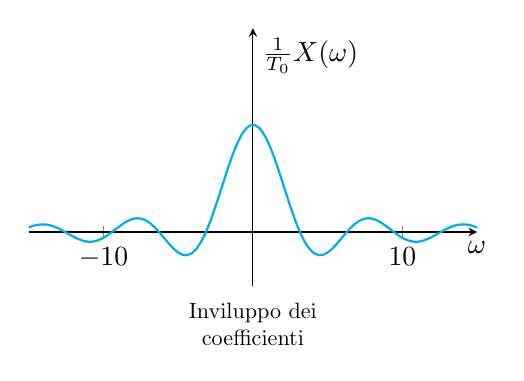
\begin{tikzpicture}
    \def\Tone{1/2}
    \def\Tzero{2.5*\Tone}
    \def\A{1}
    \begin{axis}[
      clip=false,
      width = .6\textwidth,
      height = .4\textwidth,
      ylabel = $\frac{1}{T_0}X(\omega)$,
      xlabel = $\omega$,
      xmin=-15, xmax=15,
      ymin= -0.5, ymax = \A * 1.9,
      ytick = \empty,
      axis lines = middle,
      xlabel style = {below},
      declare function ={ 
        sinc(\x) = 
        (\x == 0) * \A +
        sin(deg(\x))/\x
      ;},
      ]
      \addplot[cyan,thick,domain=-15:15,samples=100]{sinc(x)};

      \node[align=center,scale=0.8] at (axis description cs:0.5,-0.15) {Inviluppo dei\\coefficienti};
    \end{axis}
  \end{tikzpicture}
  \caption{Segnale rettangolare}
\end{figure}
\noindent
Replichiamo il segnale in un periodo \( T_0 \) e osserviamo il cambiamento dei coefficienti
di Fourier:
\begin{figure}[H]
  \centering
  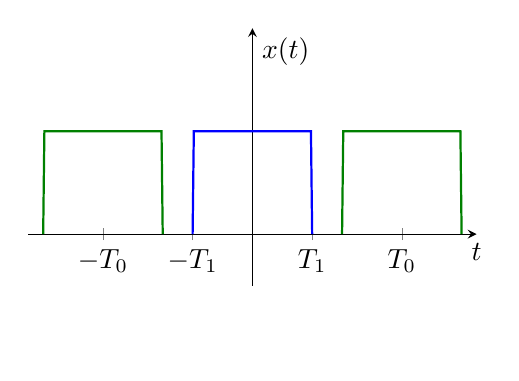
\begin{tikzpicture}
    \def\Tone{1/2}
    \def\Tzero{2.5*\Tone}
    \def\A{1}
    \begin{axis}[
      clip=false,
      width = .6\textwidth,
      height = .4\textwidth,
      ylabel = $x(t)$,
      xlabel = $t$,
      xmin=-\Tzero*1.5, xmax=\Tzero*1.5,
      ymin= -0.5, ymax = \A * 2,
      ytick = \empty,
      xtick = {-\Tzero, -\Tone, \Tone, \Tzero},
      xticklabels = {$-T_0$, $-T_1$, $T_1$, $T_0$},
      axis lines = middle,
      xlabel style = {below},
      declare function ={ 
        rect(\x) = 
        (abs(\x) > \Tone) * 0 +
        (abs(\x) == \Tone) * 0 +
        (abs(\x) < \Tone-0.0001) * \A
      ;},
      ]
      \addplot[blue,thick,domain=-\Tone:\Tone,samples=100]{rect(x)};

      \addplot[green!50!black,thick,domain=-\Tone -\Tzero:\Tone - \Tzero,samples=100]{rect(x + \Tzero)};
      \addplot[green!50!black,thick,domain=-\Tone +\Tzero:\Tone + \Tzero,samples=100]{rect(x - \Tzero)};
      \node[align=center,opacity=0,scale=0.8] at (axis description cs:0.5,-0.15) {Inviluppo dei\\coefficienti};
    \end{axis}
  \end{tikzpicture}
  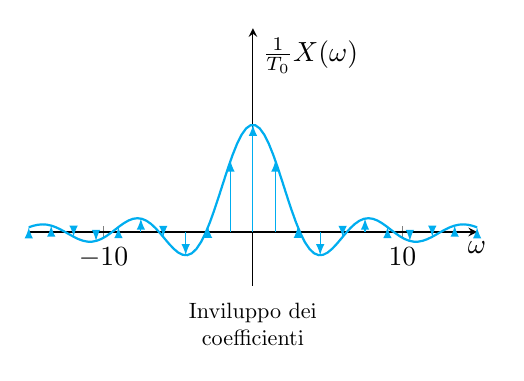
\begin{tikzpicture}
    \def\Tone{1/2}
    \def\Tzero{2.5*\Tone}
    \def\A{1}
    \begin{axis}[
      clip=false,
      width = .6\textwidth,
      height = .4\textwidth,
      ylabel = $\frac{1}{T_0}X(\omega)$,
      xlabel = $\omega$,
      xmin=-15, xmax=15,
      ymin= -0.5, ymax = \A * 1.9,
      ytick = \empty,
      axis lines = middle,
      xlabel style = {below},
      declare function ={ 
        sinc(\x) = 
        (\x == 0) * \A +
        sin(deg(\x))/\x
      ;},
      ]
      \addplot[cyan,thick,domain=-15:15,samples=100]{sinc(x)};

      \node[align=center,scale=0.8] at (axis description cs:0.5,-0.15) {Inviluppo dei\\coefficienti};

      \def\inc{1.5}
      \pgfplotsinvokeforeach{-15,-15 + \inc,...,15}{
        \draw[cyan, -latex] (axis cs:#1,0) -- (axis cs:#1,{sinc(#1)});
      }
    \end{axis}
  \end{tikzpicture}
  \caption{$T_0 = 4T_1$}
\end{figure}
\begin{figure}[H]
  \centering
  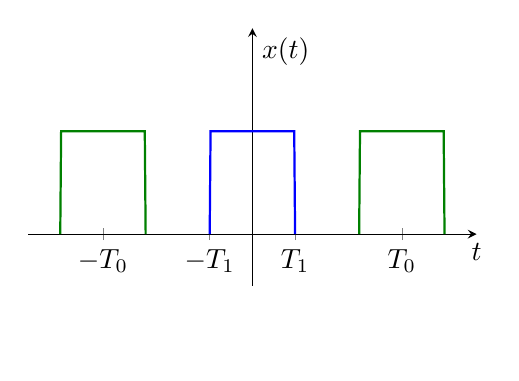
\begin{tikzpicture}
    \def\Tone{1/2}
    \def\Tzero{3.5*\Tone}
    \def\A{1}
    \begin{axis}[
      clip=false,
      width = .6\textwidth,
      height = .4\textwidth,
      ylabel = $x(t)$,
      xlabel = $t$,
      xmin=-\Tzero*1.5, xmax=\Tzero*1.5,
      ymin= -0.5, ymax = \A * 2,
      ytick = \empty,
      xtick = {-\Tzero, -\Tone, \Tone, \Tzero},
      xticklabels = {$-T_0$, $-T_1$, $T_1$, $T_0$},
      axis lines = middle,
      xlabel style = {below},
      declare function ={ 
        rect(\x) = 
        (abs(\x) > \Tone) * 0 +
        (abs(\x) == \Tone) * 0 +
        (abs(\x) < \Tone-0.0001) * \A
      ;},
      ]
      \addplot[blue,thick,domain=-\Tone:\Tone,samples=100]{rect(x)};

      \addplot[green!50!black,thick,domain=-\Tone -\Tzero:\Tone - \Tzero,samples=100]{rect(x + \Tzero)};
      \addplot[green!50!black,thick,domain=-\Tone +\Tzero:\Tone + \Tzero,samples=100]{rect(x - \Tzero)};
      \node[align=center,opacity=0,scale=0.8] at (axis description cs:0.5,-0.15) {Inviluppo dei\\coefficienti};
    \end{axis}
  \end{tikzpicture}
  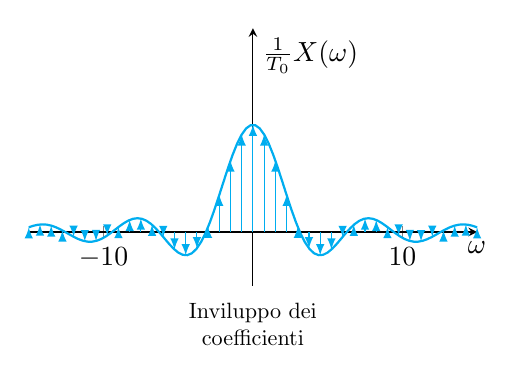
\begin{tikzpicture}
    \def\Tone{1/2}
    \def\Tzero{2.5*\Tone}
    \def\A{1}
    \begin{axis}[
      clip=false,
      width = .6\textwidth,
      height = .4\textwidth,
      ylabel = $\frac{1}{T_0}X(\omega)$,
      xlabel = $\omega$,
      xmin=-15, xmax=15,
      ymin= -0.5, ymax = \A * 1.9,
      ytick = \empty,
      axis lines = middle,
      xlabel style = {below},
      declare function ={ 
        sinc(\x) = 
        (\x == 0) * \A +
        sin(deg(\x))/\x
      ;},
      ]
      \addplot[cyan,thick,domain=-15:15,samples=100]{sinc(x)};

      \node[align=center,scale=0.8] at (axis description cs:0.5,-0.15) {Inviluppo dei\\coefficienti};

      \def\inc{0.75}
      \pgfplotsinvokeforeach{-15,-15 + \inc,...,15}{
        \draw[cyan, -latex] (axis cs:#1,0) -- (axis cs:#1,{sinc(#1)});
      }
    \end{axis}
  \end{tikzpicture}
  \caption{$T_0 = 8T_1$}
\end{figure}
\[
\ldots
\] 
\begin{figure}[H]
  \centering
  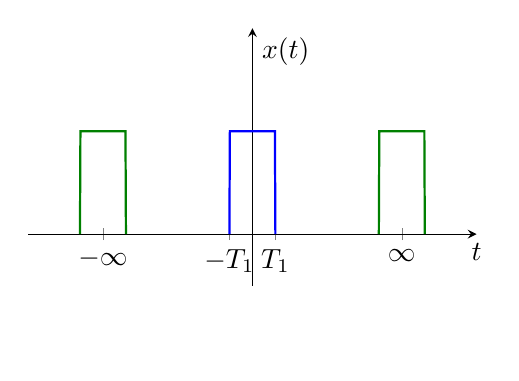
\begin{tikzpicture}
    \def\Tone{1/2}
    \def\Tzero{6.5*\Tone}
    \def\A{1}
    \begin{axis}[
      clip=false,
      width = .6\textwidth,
      height = .4\textwidth,
      ylabel = $x(t)$,
      xlabel = $t$,
      xmin=-\Tzero*1.5, xmax=\Tzero*1.5,
      ymin= -0.5, ymax = \A * 2,
      ytick = \empty,
      xtick = {-\Tzero, -\Tone, \Tone, \Tzero},
      xticklabels = {$-\infty$, $-T_1$, $T_1$, $\infty$},
      axis lines = middle,
      xlabel style = {below},
      declare function ={ 
        rect(\x) = 
        (abs(\x) > \Tone) * 0 +
        (abs(\x) == \Tone) * 0 +
        (abs(\x) < \Tone-0.0001) * \A
      ;},
      ]
      \addplot[blue,thick,domain=-\Tone:\Tone,samples=100]{rect(x)};

      \addplot[green!50!black,thick,domain=-\Tone -\Tzero:\Tone - \Tzero,samples=100]{rect(x + \Tzero)};
      \addplot[green!50!black,thick,domain=-\Tone +\Tzero:\Tone + \Tzero,samples=100]{rect(x - \Tzero)};
      \node[align=center,opacity=0,scale=0.8] at (axis description cs:0.5,-0.15) {Inviluppo dei\\coefficienti};
    \end{axis}
  \end{tikzpicture}
  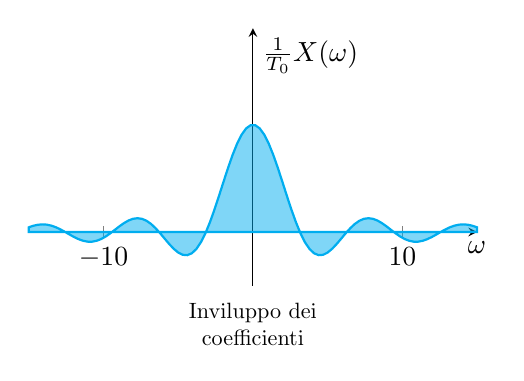
\begin{tikzpicture}
    \def\Tone{1/2}
    \def\Tzero{2.5*\Tone}
    \def\A{1}
    \begin{axis}[
      clip=false,
      width = .6\textwidth,
      height = .4\textwidth,
      ylabel = $\frac{1}{T_0}X(\omega)$,
      xlabel = $\omega$,
      xmin=-15, xmax=15,
      ymin= -0.5, ymax = \A * 1.9,
      ytick = \empty,
      axis lines = middle,
      xlabel style = {below},
      declare function ={ 
        sinc(\x) = 
        (\x == 0) * \A +
        sin(deg(\x))/\x
      ;},
      ]
      \addplot[cyan,thick,fill=cyan,fill opacity=0.5,domain=-15:15,samples=100]{sinc(x)} \closedcycle;

      \node[align=center,scale=0.8] at (axis description cs:0.5,-0.15) {Inviluppo dei\\coefficienti};
    \end{axis}
  \end{tikzpicture}
  \caption{$T_0 \to \infty$}
\end{figure}

\subsubsection{Trasformata di Fourier di un segnale periodico}
\[
  \begin{aligned}
    \tilde{v}(t) \leftrightarrow a_k \quad \text{Coefficienti delle serie di fourier}\\
    \tilde{v}(t) \stackrel{\mathcal{F}}{\leftrightarrow} \tilde{V}(\omega) \quad \text{Trasformata di Fourier}\\
    \tilde{v}(t) := \sum_{k=-\infty}^{+\infty} 2 \pi a_k \cdot \delta(\omega - k \omega_0) \text{ Treno di impulsi}\\
  \end{aligned}
\] 
\[
  \begin{aligned}
    \tilde{v}(t) &= \frac{1}{2 \pi } \int_{-\infty}^{+\infty} \tilde{V}(\omega) \cdot e^{j \omega t} \, d\omega\\
                 &= \frac{1}{2 \pi } \sum_{k=-\infty}^{+\infty} 2 \pi a_k \cdot
                 \underbrace{\int_{-\infty}^{+\infty} \delta(\omega - k \omega_0) \cdot e^{-j \omega t} \, d\omega}_{e^{-j k \omega_0 t}}
  \end{aligned}
\] 

\subsubsection{Come usare la trasformata di Fourier}
\begin{enumerate}
  \item \( v(t) \) non periodico
    \begin{itemize}
      \item Costruisco un segnale periodico \( \tilde{v}(T) \) in cui il singolo periodo
        è definito da \( v(t) \)
      \item \( \tilde{v}(t) \) ha serie di fourier
      \item All'aumentare del periodo $\tilde{v}(t) \to v(t)$ e la serie di Fourier di
        \( \tilde{v}(t) \to TdF \) di \( v(t) \) 
    \end{itemize}

  \item \( \tilde{v}(t) \) è periodico, \( v(t) \) rappresenta il singolo periodo
    \begin{itemize}
      \item Coefficienti della serie di Fourier \( = \frac{1}{T_0} \cdot \text{campioni delle
        TdF di } v(t) \)
    \end{itemize}

  \item \( \tilde{v}(t) \) è periodico
    \begin{itemize}
      \item La trasformata di Fourier di \( \tilde{v}(t) \) è definita come \textbf{treno
        di impulsi}
        \[
          \tilde{V}(\omega) = \sum_{k=-\infty}^{+\infty} 2 \pi a_k \cdot \delta(\omega - k \omega_0)
        \] 
        \begin{figure}[H]
          \centering
          \def\A{1}
          \def\xmin{-4}
          \def\xmax{4}
          \begin{tikzpicture}
            \begin{axis}[
              clip = false,
              height = 0.4\textwidth,
              ylabel = \(v(t)\),
              xlabel = \(t\),
              xmin= \xmin, xmax= \xmax,
              ymin= 0, ymax = 1.5,
              ytick = \empty,
              xtick = \empty,
              axis lines = middle,
              ]
              \addplot[-latex,blue,ultra thick] coordinates {
                  (0,0) (0,\A)
                } node[above right,scale=0.9] {$v(t)$ non periodico};
            \end{axis}
          \end{tikzpicture}
          \scalebox{2}{\( \stackrel{\mathcal{F}}{\leftrightarrow} \)}
          \begin{tikzpicture}
            \begin{axis}[
              clip = false,
              height = 0.4\textwidth,
              ylabel = \(V(\omega)\),
              xlabel = \(\omega\),
              xmin= \xmin, xmax= \xmax,
              ymin= 0, ymax = 1.5,
              ytick = \empty,
              xtick = \empty,
              axis lines = middle,
              ]
              \addplot[cyan,thick] coordinates {
                  (\xmin,\A) (\xmax,\A)
                };
            \end{axis}
          \end{tikzpicture}
        \end{figure}
        \noindent
        Se \( T_0 \to \infty\) allora il treno di impulsi diventa sempre più fitto fino
        ad una retta costante:
        \begin{figure}[H]
          \centering
          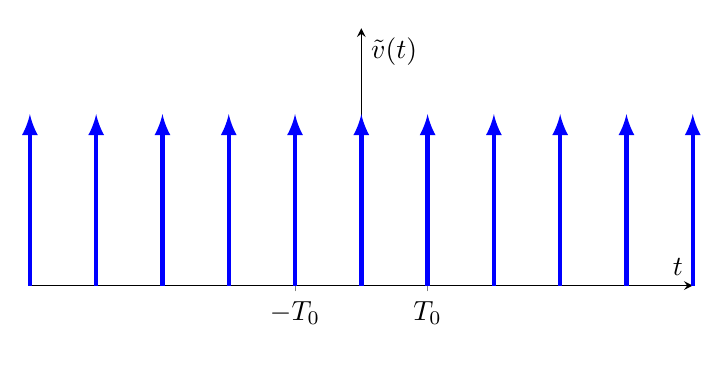
\begin{tikzpicture}
            \def\A{1}
            \def\xmin{-10}
            \def\xmax{10}
            \def\Tzero{2}
            \begin{axis}[
              clip = false,
              height = 0.4\textwidth,
              ylabel = \(\tilde{v}(t)\),
              xlabel = \(t\),
              xmin= \xmin, xmax= \xmax,
              ymin= 0, ymax = 1.5,
              ytick = \empty,
              xtick = {-\Tzero,\Tzero},
              xticklabels = {\(-T_0\),\(T_0\)},
              axis lines = middle,
              ]
              \pgfplotsinvokeforeach{0,\Tzero,...,\xmax-0.5}{
                \addplot[-latex,blue,domain=\xmin:\xmax,ultra thick] coordinates {
                    (#1,0) (#1,\A)
                  };
              }

              \pgfplotsinvokeforeach{-\Tzero, -2*\Tzero,...,\xmin+0.5}{
                \addplot[-latex,blue,domain=\xmin:\xmax,ultra thick] coordinates {
                    (#1,0) (#1,\A)
                  };
              }

              \draw[opacity=0] (axis cs:0,0) -- (axis cs:0,-0.1) 
                -- (axis cs:{(2*pi)/\Tzero},-0.1)
                node[midway, below] {\(\frac{2\pi}{T_0}\)} -- (axis cs:{(2*pi)/\Tzero},0);
            \end{axis}
          \end{tikzpicture}
          \scalebox{2}{\( \stackrel{\mathcal{F}}{\leftrightarrow} \)}
          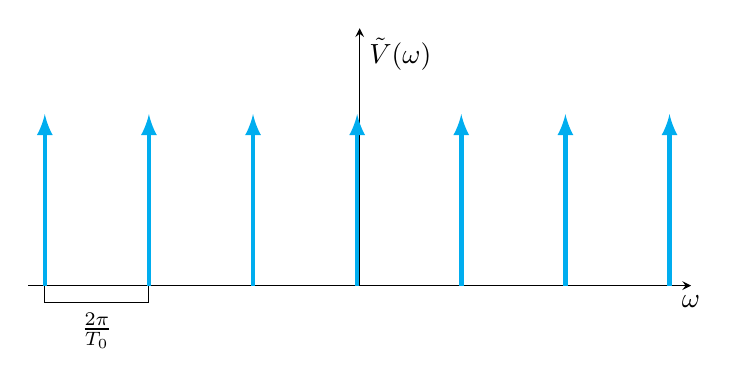
\begin{tikzpicture}
            \def\A{1}
            \def\xmin{-10}
            \def\xmax{10}
            \def\Tzero{2}
            \begin{axis}[
              clip = false,
              height = 0.4\textwidth,
              ylabel = \(\tilde{V}(\omega)\),
              xlabel = \(\omega\),
              xmin= \xmin, xmax= \xmax,
              ymin= 0, ymax = 1.5,
              ytick = \empty,
              xtick = \empty,
              axis lines = middle,
              xlabel style = {below},
              ]

              \def\inc{(2*pi)/\Tzero}
              \pgfplotsinvokeforeach{\xmin+0.5,\xmin+0.5 + \inc,...,\xmax}{
                \addplot[-latex,cyan,domain=\xmin:\xmax,ultra thick] coordinates {
                    (#1,0) (#1,\A)
                  };
              }

              \draw (axis cs:\xmin+0.5,0) -- (axis cs:\xmin+0.5,-0.1) 
                -- (axis cs:{\xmin+0.5+(2*pi)/\Tzero},-0.1)
                node[midway, below] {\(\frac{2\pi}{T_0}\)} -- (axis cs:{\xmin+0.5+(2*pi)/\Tzero},0);
            \end{axis}
          \end{tikzpicture}
        \end{figure}
        \begin{figure}[H]
          \centering
          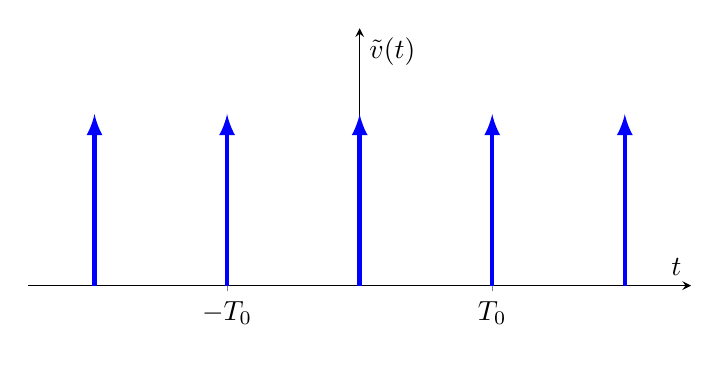
\begin{tikzpicture}
            \def\A{1}
            \def\xmin{-10}
            \def\xmax{10}
            \def\Tzero{4}
            \begin{axis}[
              clip = false,
              height = 0.4\textwidth,
              ylabel = \(\tilde{v}(t)\),
              xlabel = \(t\),
              xmin= \xmin, xmax= \xmax,
              ymin= 0, ymax = 1.5,
              ytick = \empty,
              xtick = {-\Tzero,\Tzero},
              xticklabels = {\(-T_0\),\(T_0\)},
              axis lines = middle,
              ]
              \pgfplotsinvokeforeach{0,\Tzero,...,\xmax-0.5}{
                \addplot[-latex,blue,domain=\xmin:\xmax,ultra thick] coordinates {
                    (#1,0) (#1,\A)
                  };
              }

              \pgfplotsinvokeforeach{-\Tzero, -2*\Tzero,...,\xmin+0.5}{
                \addplot[-latex,blue,domain=\xmin:\xmax,ultra thick] coordinates {
                    (#1,0) (#1,\A)
                  };
              }

              \draw[opacity=0] (axis cs:0,0) -- (axis cs:0,-0.1) 
                -- (axis cs:{(2*pi)/\Tzero},-0.1)
                node[midway, below] {\(\frac{2\pi}{T_0}\)} -- (axis cs:{(2*pi)/\Tzero},0);
            \end{axis}
          \end{tikzpicture}
          \scalebox{2}{\( \stackrel{\mathcal{F}}{\leftrightarrow} \)}
          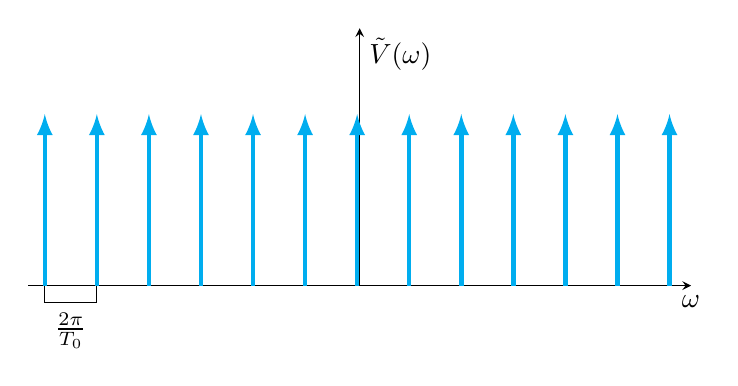
\begin{tikzpicture}
            \def\A{1}
            \def\xmin{-10}
            \def\xmax{10}
            \def\Tzero{4}
            \begin{axis}[
              clip = false,
              height = 0.4\textwidth,
              ylabel = \(\tilde{V}(\omega)\),
              xlabel = \(\omega\),
              xmin= \xmin, xmax= \xmax,
              ymin= 0, ymax = 1.5,
              ytick = \empty,
              xtick = \empty,
              axis lines = middle,
              xlabel style = {below},
              ]

              \def\inc{(2*pi)/\Tzero}
              \pgfplotsinvokeforeach{\xmin+0.5,\xmin+0.5 + \inc,...,\xmax}{
                \addplot[-latex,cyan,domain=\xmin:\xmax,ultra thick] coordinates {
                    (#1,0) (#1,\A)
                  };
              }

              \draw (axis cs:\xmin+0.5,0) -- (axis cs:\xmin+0.5,-0.1) 
                -- (axis cs:{\xmin+0.5+(2*pi)/\Tzero},-0.1)
                node[midway, below] {\(\frac{2\pi}{T_0}\)} -- (axis cs:{\xmin+0.5+(2*pi)/\Tzero},0);
            \end{axis}
          \end{tikzpicture}
        \end{figure}
        \begin{figure}[H]
          \centering
          \begin{tikzpicture}
            \def\A{1}
            \def\xmin{-10}
            \def\xmax{10}
            \def\Tzero{8}
            \begin{axis}[
              clip = false,
              height = 0.4\textwidth,
              ylabel = \(\tilde{v}(t)\),
              xlabel = \(t\),
              xmin= \xmin, xmax= \xmax,
              ymin= 0, ymax = 1.5,
              ytick = \empty,
              xtick = {-\Tzero,\Tzero},
              xticklabels = {\(-\infty\),\(\infty\)},
              axis lines = middle,
              ]
              \pgfplotsinvokeforeach{0,\Tzero,...,\xmax-0.5}{
                \addplot[-latex,blue,domain=\xmin:\xmax,ultra thick] coordinates {
                    (#1,0) (#1,\A)
                  };
              }

              \pgfplotsinvokeforeach{-\Tzero, -2*\Tzero,...,\xmin+0.5}{
                \addplot[-latex,blue,domain=\xmin:\xmax,ultra thick] coordinates {
                    (#1,0) (#1,\A)
                  };
              }

              \draw[opacity=0] (axis cs:0,0) -- (axis cs:0,-0.1) 
                -- (axis cs:{(2*pi)/\Tzero},-0.1)
                node[midway, below] {\(\frac{2\pi}{T_0}\)} -- (axis cs:{(2*pi)/\Tzero},0);
            \end{axis}
          \end{tikzpicture}
          \scalebox{2}{\( \stackrel{\mathcal{F}}{\leftrightarrow} \)}
          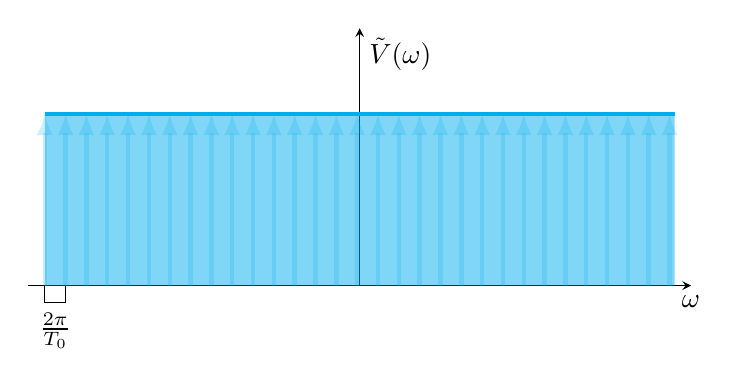
\begin{tikzpicture}
            \def\A{1}
            \def\xmin{-10}
            \def\xmax{10}
            \def\Tzero{10}
            \begin{axis}[
              clip = false,
              height = 0.4\textwidth,
              ylabel = \(\tilde{V}(\omega)\),
              xlabel = \(\omega\),
              xmin= \xmin, xmax= \xmax,
              ymin= 0, ymax = 1.5,
              ytick = \empty,
              xtick = \empty,
              axis lines = middle,
              xlabel style = {below},
              ]

              \addplot[cyan,domain=\xmin:\xmax,ultra thick] coordinates {
                  (\xmin+0.5,\A) (\xmax-0.5,\A)
                };
              \addplot[fill=cyan,fill opacity=0.5,domain=\xmin:\xmax,draw opacity=0] coordinates {
                  (\xmin+0.5,\A) (\xmax-0.5,\A)
                  (\xmax-0.5,0) (\xmin+0.5,0)
                } \closedcycle;

              \def\inc{(2*pi)/\Tzero}
              \pgfplotsinvokeforeach{\xmin+0.5,\xmin+0.5 + \inc,...,\xmax-0.5}{
                \addplot[-latex,cyan,opacity=0.2,domain=\xmin:\xmax,ultra thick] coordinates {
                    (#1,0) (#1,\A)
                  };
              }

              \draw (axis cs:\xmin+0.5,0) -- (axis cs:\xmin+0.5,-0.1) 
                -- (axis cs:{\xmin+0.5+(2*pi)/\Tzero},-0.1)
                node[midway, below] {\(\frac{2\pi}{T_0}\)} -- (axis cs:{\xmin+0.5+(2*pi)/\Tzero},0);
            \end{axis}
          \end{tikzpicture}
          \caption{Trasformata di Fourier all'aumentare di \(T_0\)}
        \end{figure}
    \end{itemize}
\end{enumerate}

% -----------------
\subsection{Condizioni di esistenza della trasformata di Fourier}
\begin{definition}[Equazione di sintesi]
  Sia \( v(t), \; t \in \mathbb{R} \) un segnale a valori reali o complessi, si definisce
  la trasformata di Fourier del segnale come:
  \[
    \mathcal{F} \left[ v(t) \right](f) := \int_{-\infty}^{+\infty} v(t) \cdot
    e^{-j \omega_0 t} \, dt = V(f)
  \] 
  Dove \( V \) è una funzione che va da \( \mathbb{R} \to \mathbb{C} \), con \( f \in \mathbb{R} \).
  Questa viene chiamata \textbf{equazione di sintesi}.
\end{definition}
\begin{definition}[Equazione di analisi]
  Data una funzione \( V: \mathbb{R} \to \mathbb{C} \) si definisce anti-trasformata di
  Fourier la funzione:
  \[
    \mathcal{F}^{-1}\left[ V(f) \right](t) := \frac{1}{2 \pi } \int_{-\infty}^{+\infty} V(f) \cdot
    e^{j \omega_0 t} \, df = v(t)
  \] 
  Dove \( v \) è una funzione che va da \( \mathbb{R} \to \mathbb{C} \), con \( t \in \mathbb{R} \).
  Questa viene chiamata \textbf{equazione di analisi}.
\end{definition}
\vspace{1em}
\noindent
\textbf{Condizioni di esistenza della trasformata di Fourier}:
\begin{theorem}
  Sia \( v(t), \; t \in \mathbb{R} \) un segnale a valori reali o complessi. Se almeno
  una delle seguenti condizioni è vera, allora la funzione è trasformabile secondo
  \( \mathcal{F} \):
  \begin{enumerate}
    \item \( v(t) \) è sommabile, cioè: 
      \[
        \int_{-\infty}^{+\infty} \left| v(t) \right| \,dt < \infty
      \]
      e a variabile limitata su ogni intervallo finito di \( \mathbb{R} \), cioè è
      esprimibile come differenza di funzioni limitate non decrescenti.

    \item \( v(t) \) è un segnale di energia, cioè:
      \[
        \int_{-\infty}^{+\infty} \left| v(t) \right|^2 \, dt < \infty
      \]

    \item \( v(t) \) è un segnale di potenza, cioè:
      \[
        \lim_{T \to \infty} \frac{1}{2T} \int_{-\infty}^{+\infty} \left| v(t) \right|^2 \, dt < \infty
      \] 
      bisogna però "\textbf{finestrare}" il segnale, cioè moltiplicarlo per una
      finestra rettangolare
  \end{enumerate}
\end{theorem}

\subsection{Trasformate notevoli}
Le trasformate di Fourier notevoli sono le seguenti:
\begin{itemize}
  \item \textbf{Impulso}
    \begin{figure}[H]
      \centering
      \begin{tikzpicture}[scale=1.5]
        \draw[->] (-1.5,0) -- (1.5,0) node[right] {$t$};
        \draw[->] (0,-0.1) -- (0,1.5) node[above] {$v(t)$};

        \draw[-latex,blue,thick] (0,0) -- (0,1) node[right] {$A$};
      \end{tikzpicture}
      \caption{Impulso unitario}
    \end{figure}
    \noindent
    La trasformata di Fourier è:
    \[
      \begin{aligned}
        \mathcal{F}\left[ A \delta_0(t) \right](f) &= A 
        \int_{-\infty}^{+\infty} \delta_0(t) \cdot e^{-j 2 \pi f t} \, dt\\
                                                   &= A \int_{-\infty}^{+\infty}
                                                   \delta_0(t) \cdot 1 \, dt\\
                                                   &= A
      \end{aligned}
    \] 
    (per le regole del campionamento)
    \begin{figure}[H]
      \centering
      \begin{tikzpicture}[scale=1.5]
        \draw[->] (-1.5,0) -- (1.5,0) node[right] {$f$};
        \draw[->] (0,-0.1) -- (0,1.5) node[above] {$V(\omega)$};

        \draw[cyan,thick] (-1.5,1) -- (1.5,1) node[right] {$A$};
      \end{tikzpicture}
      \caption{Trasformata di Fourier dell'impulso}
    \end{figure}


  \item \textbf{Esponenziale causale}
    \begin{figure}[H]
      \centering
      \begin{tikzpicture}
        \begin{axis}[
          axis lines = middle,
          xmin= 0, xmax= 6,
          ymin= 0, ymax = 6,
          ylabel = $v(t)$,
          xlabel = $t$,
          xtick = \empty,
          ytick = \empty,
          xlabel style = {below},
          ylabel style = {left},
          ]
          \addplot[blue,thick,domain=0:6, samples=50]{exp(x/2)};
          \addplot[red,thick,domain=0:6, samples=50]{exp(-x/2)};
        \end{axis}
      \end{tikzpicture}
      \caption{Esponenziale causale}
    \end{figure}
    \noindent
    La trasformata di Fourier è:
    \[
      \mathcal{F}\left[ A e^{j \phi} e^{\lambda t} 
      \underbrace{\delta_{-1}(t)}_{\text{Causalità}} \right](t) =
      \frac{A e^{j \phi}}{j 2 \pi  f - \lambda}
    \] 

    \vspace{1em}
    \noindent
    La trasformata di Laplace è molto simile, basta infatti sostituire la \( s \) 
    con \( j \omega = j 2 \pi f \) e si ottiene la trasformata di Fourier:
    \[
      \mathcal{L}\left[ A e^{j \phi} e^{\lambda t} 
      \delta_{-1}(t) \right](s) = \frac{A e^{j \phi}}{s - \lambda}
    \] 


  \item \textbf{Finestra rettangolare di altezza \( A \) e supporto \( T \)}
    \begin{figure}[H]
      \centering
      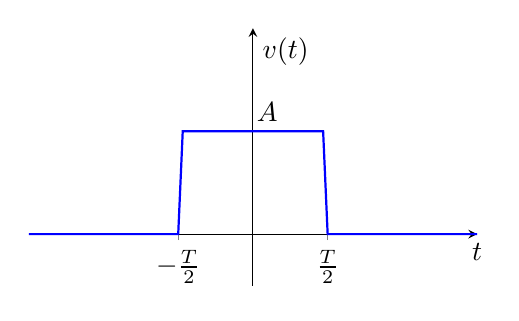
\begin{tikzpicture}
        \def\T{1/2}
        \def\xmin{-\T*3}
        \def\xmax{\T*3}
        \def\A{1}
        \begin{axis}[
          clip=false,
          width = .6\textwidth,
          height = .4\textwidth,
          ylabel = $v(t)$,
          xlabel = $t$,
          xmin=\xmin, xmax=\xmax,
          ymin= -0.5, ymax = \A * 2,
          ytick = {\A},
          yticklabels = {$A$},
          yticklabel style = {above right},
          xtick = {-\T, \T},
          xticklabels = {$-\frac{T}{2}$, $\frac{T}{2}$},
          axis lines = middle,
          xlabel style = {below},
          declare function ={ 
            rect(\x) = 
            (abs(\x) > \T) * 0 +
            (abs(\x) == \T) * 0 +
            (abs(\x) < \T-0.0001) * \A
          ;},
          ]
          \addplot[blue,thick,domain=\xmin:\xmax,samples=100]{rect(x)};
        \end{axis}
      \end{tikzpicture}
      \caption{Finestra rettangolare}
    \end{figure}
    \noindent
    La trasformata di Fourier è:
    \[
      \mathcal{F}\left[ A \Pi\left(\frac{t}{T}\right) \right](f) = AT \cdot sinc(fT)
    \]
    \begin{figure}[H]
      \centering
      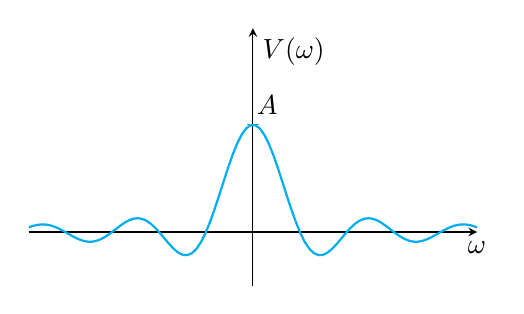
\begin{tikzpicture}
        \def\Tone{1/2}
        \def\Tzero{2.5*\Tone}
        \def\A{1}
        \begin{axis}[
          clip=false,
          width = .6\textwidth,
          height = .4\textwidth,
          ylabel = $V(\omega)$,
          xlabel = $\omega$,
          xmin=-15, xmax=15,
          ymin= -0.5, ymax = \A * 1.9,
          ytick = {\A},
          yticklabels = {$A$},
          yticklabel style = {above right},
          xtick = \empty,
          axis lines = middle,
          xlabel style = {below},
          declare function ={ 
            sinc(\x) = 
            (\x == 0) * \A +
            sin(deg(\x))/\x
          ;},
          ]
          \addplot[cyan,thick,domain=-15:15,samples=100]{sinc(x)};
        \end{axis}
      \end{tikzpicture}
      \caption{Trasformata di Fourier della finestra rettangolare}
    \end{figure}
    \noindent
    Questa funzione è chiamata \textbf{sinc}.


  \item \textbf{Funzione costante}
    \vspace{1em}
    \noindent
    \begin{figure}[H]
      \centering
      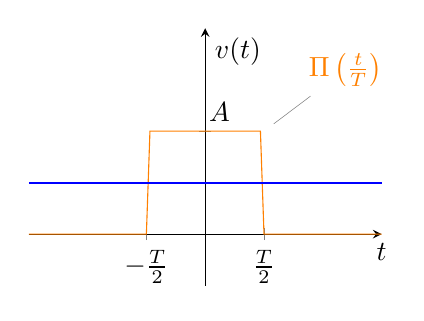
\begin{tikzpicture}
        \def\T{1/2}
        \def\xmin{-\T*3}
        \def\xmax{\T*3}
        \def\A{1}
        \begin{axis}[
          clip=false,
          width = .5\textwidth,
          height = .4\textwidth,
          ylabel = $v(t)$,
          xlabel = $t$,
          xmin=\xmin, xmax=\xmax,
          ymin= -0.5, ymax = \A * 2,
          ytick = {\A},
          yticklabels = {$A$},
          yticklabel style = {above right},
          xtick = {-\T, \T},
          xticklabels = {$-\frac{T}{2}$, $\frac{T}{2}$},
          axis lines = middle,
          xlabel style = {below},
          declare function ={ 
            rect(\x) = 
            (abs(\x) > \T) * 0 +
            (abs(\x) == \T) * 0 +
            (abs(\x) < \T-0.0001) * \A
          ;},
          ]
          \addplot[orange,domain=\xmin:\xmax,samples=100]{rect(x)};

          \addplot[blue,thick,domain=\xmin:\xmax]{\A/2};

          \node[pin={[orange]45:{$\Pi\left( \frac{t}{T} \right)$}}] at (axis cs:\T,\A) {};
        \end{axis}
      \end{tikzpicture}
      \scalebox{2}{\( \to \)}
      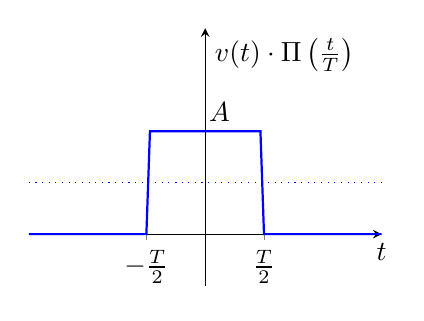
\begin{tikzpicture}
        \def\T{1/2}
        \def\xmin{-\T*3}
        \def\xmax{\T*3}
        \def\A{1}
        \begin{axis}[
          clip=false,
          width = .5\textwidth,
          height = .4\textwidth,
          ylabel = $v(t) \cdot \Pi \left( \frac{t}{T} \right) $,
          xlabel = $t$,
          xmin=\xmin, xmax=\xmax,
          ymin= -0.5, ymax = \A * 2,
          ytick = {\A},
          yticklabels = {$A$},
          yticklabel style = {above right},
          xtick = {-\T, \T},
          xticklabels = {$-\frac{T}{2}$, $\frac{T}{2}$},
          axis lines = middle,
          xlabel style = {below},
          declare function ={ 
            rect(\x) = 
            (abs(\x) > \T) * 0 +
            (abs(\x) == \T) * 0 +
            (abs(\x) < \T-0.0001) * \A
          ;},
          ]
          \addplot[blue,thick,domain=\xmin:\xmax,samples=100]{rect(x)};

          \addplot[blue,dotted,thin,domain=\xmin:\xmax]{\A/2};
        \end{axis}
      \end{tikzpicture}
      \caption{Funzione costante}
    \end{figure}
    La funzione costante non può essere trasformata facilmente, quindi bisogna
    "finestrarla", cioè moltiplicare il segnale per una finestra rettangolare:
    \[
    v(t) = A \to v_T(t) = A \cdot \Pi(\frac{t}{T})
    \] 
    La sua trasformata di Fourier è la stessa del segnale rettangolare:
    \[
      \mathcal{F}\left[\underbrace{v(t)}_{\text{Ampiezza } = A} \cdot 
      \underbrace{\Pi\left(\frac{t}{T}\right)}_{\text{Ampiezza } = 1} \right](f)
      = AT \cdot sinc(fT)
    \] 
    \begin{figure}[H]
      \centering
      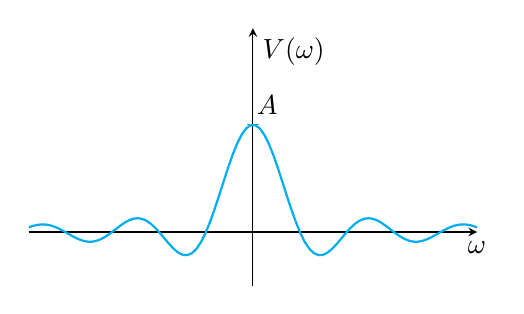
\begin{tikzpicture}
        \def\Tone{1/2}
        \def\Tzero{2.5*\Tone}
        \def\A{1}
        \begin{axis}[
          clip=false,
          width = .6\textwidth,
          height = .4\textwidth,
          ylabel = $V(\omega)$,
          xlabel = $\omega$,
          xmin=-15, xmax=15,
          ymin= -0.5, ymax = \A * 1.9,
          ytick = {\A},
          yticklabels = {$A$},
          yticklabel style = {above right},
          xtick = \empty,
          axis lines = middle,
          xlabel style = {below},
          declare function ={ 
            sinc(\x) = 
            (\x == 0) * \A +
            sin(deg(\x))/\x
          ;},
          ]
          \addplot[cyan,thick,domain=-15:15,samples=100]{sinc(x)};
        \end{axis}
      \end{tikzpicture}
      \caption{Trasformata di Fourier della funzione costante}
    \end{figure}


  \item \textbf{Fasore}
    \begin{figure}[H]
      \centering
      \begin{tikzpicture}[scale=1.5]
        \draw[->] (-1.5,0) -- (1.5,0) node[right] {$\Re$};
        \draw[->] (0,-1.5) -- (0,1.5) node[above] {$\Im$};

        \draw (0,0) circle (1);

        \draw[blue,thick,->] (1,0) arc (0:60:1);
      \end{tikzpicture}
      \caption{Fasore}
    \end{figure}
    \[
      v(t) = A \cdot e^{j 2 \pi f_0 t}
    \] 
    Anche in questo caso bisogna moltiplicare per il segnale rettangolare:
    \[
      v_T(t) = A \cdot e^{j 2 \pi f_0 t} \cdot \Pi\left(\frac{t}{T}\right)
    \] 
    La trasformata di Fourier è:
    \[
      \mathcal{F}\left[ v_T(t) \right](f) = AT \cdot sinc((f - f_0) \cdot t)
    \] 
    \begin{figure}[H]
      \centering
      \begin{tikzpicture}
        \def\Fzero{7}
        \def\A{1}
        \begin{axis}[
          clip=false,
          width = .6\textwidth,
          height = .4\textwidth,
          ylabel = $V(\omega)$,
          xlabel = $\omega$,
          xmin=-15, xmax=15,
          ymin= -0.5, ymax = \A * 1.9,
          ytick = {\A},
          yticklabels = {$A$},
          yticklabel style = {above right},
          xtick = \empty,
          axis lines = middle,
          xlabel style = {below},
          declare function ={ 
            sinc(\x) = 
            (\x == 0) * \A +
            sin(deg(\x))/\x
          ;},
          ]
          \addplot[cyan,thick,domain=-15:15,samples=100]{sinc(x - \Fzero)};

          \draw[dashed] (axis cs:\Fzero,\A) -- (axis cs:\Fzero,0) node[below] {$f_0$};
        \end{axis}
      \end{tikzpicture}
      \caption{Trasformata di Fourier del fasore}
    \end{figure}
  \item \textbf{Seno}
    \vspace{1em}
    \noindent
    Possiamo derivare il seno utilizzando la formula di Eulero su un fasore:
    \[
    v(t) = A \cdot \sin(2 \pi f_0 t)
    \] 
    La trasformata di Fourier è:
    \[
      \mathcal{F}\left[ v(t) \right](f) = \frac{A}{2j} \left( \delta(f - f_0) - \delta(f + f_0) \right)
    \]
    Il seno è solo la parte immaginaria del fasore.
  \item \textbf{Coseno}
    \vspace{1em}
    \noindent
    \[
    v(t) = A \cdot \cos(2 \pi f_0 t)
    \] 
    La trasformata di Fourier è:
    \[
      \mathcal{F}\left[ v(t) \right](f) = \frac{A}{2} \left( \delta(f - f_0) + \delta(f + f_0) \right)
    \]
    Il coseno è solo la parte reale del fasore.
\end{itemize}

\subsection{Proprietà della trasformata di Fourier}
La trasformata di Laplace è un caso specifico della trasformata di Fourier:
\[
\begin{aligned}
  TdL &\to TdF\\
  s &\to j \omega
\end{aligned}
\] 
Quindi alcune proprietà di Laplace valgono anche per Fourier.
\begin{enumerate}
  \item \textbf{Linearità}
    \[
      a v_1(t) + b v_2(t) \stackrel{\mathcal{F}}{\leftrightarrow} a V_1(f) + b V_2(f)
    \] 

  \item \textbf{Riflessione e coniugazione}
    \[
      v(-t) \stackrel{\mathcal{F}}{\leftrightarrow} V(-f) \quad \text{Riflessione}
    \] 
    \[
      \left.
      \begin{aligned}
        v^*(t) \stackrel{\mathcal{F}}{\leftrightarrow} V^*(-f)\\
        v^*(-t) \stackrel{\mathcal{F}}{\leftrightarrow} V^*(f)
      \end{aligned}
    \right\}
    \text{ Coniugazione}
    \]

  \item \textbf{Convoluzione nel dominio del tempo}
    \[
      \left[ v_1 \ast v_2 \right](t) \stackrel{\mathcal{F}}{\leftrightarrow} V_1(f) \cdot V_2(f)
    \] 

  \item \textbf{Traslazione nel dominio del tempo}
    \[
      v(t - \tau) \stackrel{\mathcal{F}}{\leftrightarrow} e^{-j 2 \pi f \tau} \cdot V(f)
    \] 

  \item \textbf{Traslazione nel dominio delle frequenze}
    \[
      e^{j 2 \pi f_0 t} \cdot v(t) \stackrel{\mathcal{F}}{\leftrightarrow} V(f - f_0)
    \]

  \item \textbf{Modulazione/Prodotto nel dominio del tempo}
    \[
      v_1(t) \cdot v_2(t) \stackrel{\mathcal{F}}{\leftrightarrow} \left[ V_1 \ast V_2 \right](f)
    \]
\end{enumerate}

\begin{examplebox}{Esempio}
  Consideriamo il seguente sistema a blocchi:
  \begin{figure}[H]
    \centering
    \begin{tikzpicture}
      \node (u) {$u(t)$};
      \node[right=of u,circle,draw,minimum size=0.7cm] (mul) {$X$};
      \node[below=of mul] (w) {$w(t)$};
      \node[right=of mul,draw,minimum size=1cm] (h) {$h(t)$};

      \draw[->] (u) -- (mul);
      \draw[->] (w) -- (mul);
      \draw[->] (mul) -- (h) node[midway,above] {$\color{blue}a(t)$};
      \draw[->] (h) -- ++(1.5,0) node[midway,above] {$\color{blue}b(t)$};

      \node[pin={[align=center,scale=0.8]above:{Convoluzione nelle frequenze/\\Prodotto nel tempo}}]
        at (mul.north) {};
      \node[pin={[align=center,scale=0.8,xshift=0.4cm]below:{Prodotti nelle frequenze/\\Convoluzioni nel tempo}}]
        at (h.south) {};
    \end{tikzpicture}
    \caption{Sistema a blocchi}
  \end{figure}
  \noindent
  Vogliamo capire come si comporta questo segnale nelle frequenze ($a(t)$) e cosa succede quando
  viene alterato dalla sequenza degli operatori ($b(t)$).
  \[
    \begin{aligned}
      u(t) &= 3 \cdot \cos(6 \pi t) + \cos(2 \pi t)\\
      w(t) &= 2 \cdot \cos(4 \pi t) \\
      h(t) &= 4 \cdot sinc(4t)\\
      \color{blue}b(t) &= ?
    \end{aligned}
  \] 
  Possiamo risolvere in maniera grafica questo problema:
  \begin{enumerate}
    \item Applichiamo le trasformate di Fourier per andare nel dominio delle frequenze:
      \[
      \text{Trasformata notevole: } A \cos(2 \pi f_0 t) = \frac{A}{2} \left( \delta(f - f_0) + \delta(f + f_0) \right)
      \] 
      \[
        \begin{aligned}
          3 \cdot \cos(2 \pi \cdot 3 \cdot t) \stackrel{\mathcal{F}}{=} \frac{3}{2} \left( \delta(f - 3) + \delta(f + 3) \right)\\
          \cos(2 \pi \cdot t) \stackrel{\mathcal{F}}{=} \frac{1}{2} \left( \delta(f - 1) + \delta(f + 1) \right)\\
          U(f) = \frac{3}{2} \left( \delta(f - 3) + \delta(f + 3) \right) + \frac{1}{2} \left( \delta(f - 1) + \delta(f + 1) \right)
        \end{aligned}
      \] 
      \vspace{1em}
      \noindent
      \[
      W(f) = \frac{2}{2} \left( \delta(f - 2) + \delta(f + 2) \right) 
      = \delta(f - 2) + \delta(f + 2)
      \] 
      \vspace{1em}
      \noindent
      \[
        \text{Trasformata notevole: } AT sinc(tT) = A \Pi\left(\frac{f}{T}\right)
      \] 
      \[
        H(f) = 1 \cdot \Pi(\frac{f}{4}) = \Pi(\frac{f}{4})
      \] 

    \item Disegnamo tutti i singoli elementi su un grafico:
      \begin{figure}[H]
        \centering
        \begin{tikzpicture}
          \begin{axis}[
            width=0.8\textwidth,
            height=0.4\textwidth,
            xlabel = $f$,
            ylabel = $U(f)$,
            xmin= -6, xmax=6,
            ymin= 0, ymax = 3,
            xtick = {-3,-1,1,3},
            ytick = {1/2,3/2},
            yticklabels = {$\frac{1}{2}$,$\frac{3}{2}$},
            axis lines = middle,
            ]
            \addplot[-latex,blue,thick] coordinates {
                (-3,0) (-3,3/2)
              };
            \addplot[-latex,blue,thick] coordinates {
                (-1,0) (-1,1/2)
              };
            \addplot[-latex,blue,thick] coordinates {
                (1,0) (1,1/2)
              };
            \addplot[-latex,blue,thick] coordinates {
                (3,0) (3,3/2)
              };
          \end{axis}
        \end{tikzpicture}
        \caption{Segnale \(U(f)\)}
      \end{figure}

      \begin{figure}[H]
        \centering
        \begin{tikzpicture}
          \begin{axis}[
            width=0.8\textwidth,
            height=0.4\textwidth,
            xlabel = $f$,
            ylabel = $W(f)$,
            xmin= -6, xmax=6,
            ymin= 0, ymax = 3,
            xtick = {-2,2},
            ytick = {1},
            axis lines = middle,
            ]
            \addplot[-latex,green!50!black,thick] coordinates {
                (-2,0) (-2,1)
              };
            \addplot[-latex,green!50!black,thick] coordinates {
                (2,0) (2,1)
              };
          \end{axis}
        \end{tikzpicture}
        \caption{Segnale \(W(f)\)}
      \end{figure}

      \begin{figure}[H]
        \centering
        \begin{tikzpicture}
          \def\T{4}
          \def\A{1}
          \begin{axis}[
            width=0.8\textwidth,
            height=0.4\textwidth,
            xlabel = $f$,
            ylabel = $H(f)$,
            xmin= -6, xmax=6,
            ymin= 0, ymax = 3,
            xtick = {-2,2},
            xticklabels = {$\underset{-\frac{T}{2}}{-2}$,$\underset{\frac{T}{2}}{2}$},
            ytick = {1},
            yticklabel style = {above left},
            axis lines = middle,
            declare function ={ 
              rect(\x) = 
              (abs(\x) > \T/2) * 0 +
              (abs(\x) == \T/2) * 0 +
              (abs(\x) < (\T/2)-0.0001) * \A
            ;},
            ]
            \addplot[magenta,thick,domain=-\T/2:\T/2,samples=100]{rect(x)};
          \end{axis}
        \end{tikzpicture}
        \caption{Segnale \(H(f)\)}
      \end{figure}

    \item Calcoliamo la convoluzione tra \( U(f) \) e \( W(f) \) per trovare \( A(f) \) :
      \vspace{1em}
      \noindent
      Eseguiamo la convoluzione tra \( U(f) \) e \( W(f) \) fissando un segnale e
      spostare l'altro specchiato. A livello più alto il segnale che si muove viene replicato
      ogni volta che l'asse centrale corrisponde con il segnale fermo:
      \begin{figure}[H]
        \centering
        \begin{tikzpicture}
          \begin{axis}[
            width=0.8\textwidth,
            height=0.4\textwidth,
            xlabel = $f$,
            ylabel = $\color{blue}U(f)\color{black} \ast \color{green!50!black}W(f)$,
            xmin= -6, xmax=6,
            ymin= 0, ymax = 3,
            xtick = {-5,-3,-1,1,3,5},
            ytick = {1/2,1,3/2,2},
            yticklabels = {$\frac{1}{2}$,1,$\frac{3}{2}$,2},
            axis lines = middle,
            ]


            \addplot[-latex,green!50!black,thick] coordinates {
                (-5,0) (-5,3/2)
              };
            \addplot[-latex,green!50!black,thick] coordinates {
                (-3,0) (-3,1/2)
              };
            \addplot[-latex,green!50!black,thick] coordinates {
                (-1,0) (-1,3/2)
              };
            \addplot[-latex,green!50!black,thick] coordinates {
                (-1,3/2) (-1,3/2+1/2) 
              };
            \addplot[-latex,green!50!black,thick] coordinates {
                (1,0) (1,1/2)
              };
            \addplot[-latex,green!50!black,thick] coordinates {
                (1,1/2) (1,1/2+3/2)
              };
            \addplot[-latex,green!50!black,thick] coordinates {
                (3,0) (3,1/2)
              };
            \addplot[-latex,green!50!black,thick] coordinates {
                (5,0) (5,3/2)
              };

            \addplot[-latex,blue,thin,dashed] coordinates {
                (-3,0) (-3,3/2)
              };
            \addplot[-latex,blue,thin,dashed] coordinates {
                (-1,0) (-1,1/2)
              };
            \addplot[-latex,blue,thin,dashed] coordinates {
                (1,0) (1,1/2)
              };
            \addplot[-latex,blue,thin,dashed] coordinates {
                (3,0) (3,3/2)
              };
          \end{axis}
        \end{tikzpicture}
        \[
          \Downarrow
        \] 
        \begin{tikzpicture}
          \begin{axis}[
            width=0.8\textwidth,
            height=0.4\textwidth,
            xlabel = $f$,
            ylabel = $A(f)$,
            xmin= -6, xmax=6,
            ymin= 0, ymax = 3,
            xtick = {-5,-3,-1,1,3,5},
            ytick = {1/2,3/2,2},
            yticklabels = {$\frac{1}{2}$,$\frac{3}{2}$,2},
            axis lines = middle,
            ]
            \addplot[-latex,red,thick] coordinates {
                (-5,0) (-5,3/2)
              };
            \addplot[-latex,red,thick] coordinates {
                (-3,0) (-3,1/2)
              };
            \addplot[-latex,red,thick] coordinates {
                (-1,0) (-1,3/2+1/2)
              };
            \addplot[-latex,red,thick] coordinates {
                (1,0) (1,1/2+3/2)
              };
            \addplot[-latex,red,thick] coordinates {
                (3,0) (3,1/2)
              };
            \addplot[-latex,red,thick] coordinates {
                (5,0) (5,3/2)
              };
          \end{axis}
        \end{tikzpicture}
        \caption{Segnale \(A(f)\)}
      \end{figure}
      \noindent
      Le altezze dei nuovi segnali replicati saranno la moltiplcazione dei segnali
      che si sovrappongono sommata alle altezze dei diversi segnali che si sovrappongono
      nello stesso punto.

    \item Calcoliamo il prodotto tra \( A(f) \) e \( H(f) \) per trovare \( B(f) \):
      \vspace{1em}
      \noindent
      \begin{figure}[H]
        \centering
        \begin{tikzpicture}
          \def\T{4}
          \def\A{1}
          \begin{axis}[
            width=0.8\textwidth,
            height=0.4\textwidth,
            xlabel = $f$,
            ylabel = $\color{red}A(f)\color{black}\cdot \color{magenta}H(f)$,
            xmin= -6, xmax=6,
            ymin= 0, ymax = 3,
            xtick = {-5,-3,-2,-1,1,2,3,5},
            ytick = {1/2,1,3/2,2},
            yticklabels = {$\frac{1}{2}$,,$\frac{3}{2}$,2},
            axis lines = middle,
            declare function ={ 
              rect(\x) = 
              (abs(\x) > \T/2) * 0 +
              (abs(\x) == \T/2) * 0 +
              (abs(\x) < (\T/2)-0.0001) * \A
            ;},
            ]
            \addplot[-latex,red,thick] coordinates {
                (-5,0) (-5,3/2)
              };
            \addplot[-latex,red,thick] coordinates {
                (-3,0) (-3,1/2)
              };
            \addplot[-latex,red,thick] coordinates {
                (-1,0) (-1,3/2+1/2)
              };
            \addplot[-latex,red,thick] coordinates {
                (1,0) (1,1/2+3/2)
              };
            \addplot[-latex,red,thick] coordinates {
                (3,0) (3,1/2)
              };
            \addplot[-latex,red,thick] coordinates {
                (5,0) (5,3/2)
              };

            \addplot[magenta,thick,domain=-\T/2:\T/2,samples=100]{rect(x)};
          \end{axis}
        \end{tikzpicture}
        \[
          \Downarrow
        \] 
        \begin{tikzpicture}
          \def\T{4}
          \def\A{1}
          \begin{axis}[
            width=0.8\textwidth,
            height=0.4\textwidth,
            xlabel = $f$,
            ylabel = $B(f)$,
            xmin= -6, xmax=6,
            ymin= 0, ymax = 3,
            xtick = {-1,1},
            ytick = {2},
            axis lines = middle,
            ]
            \addplot[-latex,orange,thick] coordinates {
                (-1,0) (-1,3/2+1/2)
              };
            \addplot[-latex,orange,thick] coordinates {
                (1,0) (1,1/2+3/2)
              };
          \end{axis}
        \end{tikzpicture}
        \caption{Segnale \(B(f)\)}
      \end{figure}
  \end{enumerate}
\end{examplebox}

\subsection{Campionamento e replicazione}
Prendiamo in considerazione il seguente sistema a blocchi
\begin{figure}[H]
  \centering
  \begin{tikzpicture}
    \node (u) {$u(t)$};
    \node[right=of u,circle,draw,minimum size=0.7cm] (mul) {$X$};
    \node[below=of mul] (w) {$w(t)$};
    \node[right=of mul,draw,minimum size=1cm] (h) {$h(t)$};

    \draw[->] (u) -- (mul);
    \draw[->] (w) -- (mul);
    \draw[->] (mul) -- (h) node[midway,above] {$\color{blue}a(t)$};
    \draw[->] (h) -- ++(1.5,0) node[midway,above] {$\color{blue}b(t)$};

    \node[pin={[align=center,scale=0.8]above:{Convoluzione nelle frequenze/\\Prodotto nel tempo}}]
      at (mul.north) {};
    \node[pin={[align=center,scale=0.8,xshift=0.4cm]below:{Prodotti nelle frequenze/\\Convoluzioni nel tempo}}]
      at (h.south) {};
  \end{tikzpicture}
  \caption{Sistema a blocchi}
\end{figure}
\[
  \begin{aligned}
    a(t) &= u(t) \cdot w(t)\\
    b(t) &= \left[ h(t) \ast a(t) \right](f)
  \end{aligned}
\] 
Esiste un operatore chiamato \textbf{campionatore} che si chiude a intervalli regolari
derivati da \( T_c \) (\textbf{frequenza di campionamento} [\( Hz \)]) e "compone" il
segnale. È il componente che permette di passare dal segnale a tempo continuo a quello
a tempo discreto.
\begin{figure}[H]
  \centering
  \begin{tikzpicture}[scale=1.5]
    \draw (0,0) -- ++(0.5,0) -- ++(0.5,0.5) node[midway,below,yshift=-0.2cm] {$T_c$};
    \draw (0,0) ++(0.5,0) ++(0.5,0) -- ++(0.5,0);
  \end{tikzpicture}
  \caption{Campionatore}
\end{figure}
\noindent
Quindi se prendiamo in considerazione il seguente segnale si ha un passaggio da continuo
a discreto:
\label{16-01-D1}

\vspace{1em}
\noindent
Nella realtà dopo il campionatore si inserisce uno \textbf{zero-holder} che mantiene il valore
del segnale fino al prossimo campione:
\label{16-01-D2}

\noindent
Un segnale discreto può essere \textbf{quantizzato}, cioè approssimato ad un valore
discreto. Questo processo è chiamato \textbf{quantizzazione}.

Inoltre un segnale quantizzato può essere \textbf{codificato} in binario, cioè rappresentato
da una sequenza di bit, ovvero segnali alti e bassi:
\label{16-01-D3}

\subsubsection{Treno campionatore/impulsi}
Un treno di impulsi a distanza \( T_c \) moltiplicato per un altro segnale fa ottenere
un segnale campionato in quel punto \( kT_c \):
\label{16-01-D4}
\[
  \begin{aligned}
    \hat{\delta}_{T_c}(t) &= \sum_{k = -\infty}^{\infty} \delta(t - kT_c)\\
                       &\updownarrow \mathcal{F}\\
    \frac{1}{T_c} \hat{\delta}_{\frac{1}{T_c}}(f) &= \frac{1}{T_c} \sum_{k = -\infty}^{\infty} \delta(f - \frac{k}{T_c})
  \end{aligned}
\] 

\subsubsection{Campionamento}
\begin{definition}
  Dato un segnale \( v(t), \; t \in \mathbb{R} \) e un periodo di campionamento 
  \( 0 < T_c \in \mathbb{R} \), il campionamento è deinito come:
  \[
    \left[ samp_{T_c} v \right](t) = \sum_{k = -\infty}^{\infty} v(kT_c)
  \] 
  \[
  \downarrow \text{ Per la proprietà del campionamento dell'impulso}
  \] 
  \[
    \begin{aligned}
      \left[ samp_{T_c} v \right](t) &= \sum_{k = -\infty}^{\infty} v(kT_c) \cdot \delta(t - kT_c)\\
                                     &= v(t) \cdot \hat{\hat{\delta}}_{T_c}(t)\\
    \end{aligned}
  \] 
  \label{16-01-D5}
\end{definition}

\subsubsection{Replicazione}
\begin{definition}
  Sia un segnale \( v(t), t \in \mathbb{R} \) e un periodo di campionamento \( 0 < T_c \in \mathbb{R} \),
  la replicazione è definita come:
  \[
    \begin{aligned}
      \left[ rep_{T_c} v \right](t) &= \sum_{k = -\infty}^{\infty} v(t - kT_c)\\
                                    &= \sum_{k = -\infty}^{\infty} v(t) \ast \delta(t - kT_c)\\
                                    &= \left[ v \ast \hat{\delta}_{T_C} \right](t)
    \end{aligned}
  \]
  \label{16-01-D6}
\end{definition}

\vspace{1em}
\noindent
Se si replica nel tempo si ottiene un campionamento scalato nelle frequenze
\[
  \left[ rep_{T_c} v\right](t) \stackrel{\mathcal{F}}{\leftrightarrow} \frac{1}{T_c} \left[ samp_{T_c} V \right](f)
\] 
Se si campiona nel tempo si ottiene una replicazione scalata nelle frequenze
\[
  \left[ samp_{T_c} v \right](t) \stackrel{\mathcal{F}}{\leftrightarrow} \frac{1}{T_c} \left[ rep_{T_c} V \right](f)
\] 

\subsubsection{Teorema del campionamento ideale di Shannon}
\begin{theorem}
  Sia \( v(t), \; t \in \mathbb{R} \) un segnale campionato con frequenza di campionamento
  \( f_c = \frac{1}{T_c} \) ottenendo:
  \[
    \begin{aligned}
      v(k) &= v_0(kT_c)\\
           &= \sum_{n = -\infty}^{\infty} v_0(t) \cdot \delta(t - kT_c)\\
           &= \left[ samp_{T_c} v_0 \right](t)
    \end{aligned}
  \] 
  Se:
  \begin{enumerate}
    \item \( v_0(t) \) è limitato in banda, cioè esiste almeno un \( B > 0 \) tale che
      \( V_0(f) = 0 \) per frequenze \( |f| > B \), e \( B \) è il più piccolo per cui
      questo è vero. Ad esempio:
      \label{16-01-D7}

    \item e la frequenza di campionamento \( f_c \) è tale per cui \( f_c > 2B \),
      dove \( 2B \) è detta \textbf{frequenza di Nyquist}. Ad esempio:
      \label{16-01-D8}
      Se:
      \[
      \begin{aligned}
        B &= 10 Hz\\
        f_c &= 5 Hz \\
      \end{aligned}
      \] 
      \[
        f_c > 2B \to 5 > 20 \text{ (FALSO)}
      \] 

      \vspace{1em}
      \noindent
      Se:
      \[
      \begin{aligned}
        B &= 5 Hz \\
        f_c &= 20 Hz \\
      \end{aligned}
      \] 
      \[
        f_c > 2B \to 20 > 10 \text{ (VERO)}
      \] 
  \end{enumerate}
  Allora \( v_0(t) \) è ricostruibile a partire dal segnale campionato 
  \( \left[ samp_{T_c} v_0\right](t) \) utilizzando un filtro di ricostruzione \( H_r \):
  \[
  H_r(f) = T_c \Pi \left( \frac{f}{2f_L} \right) = \frac{1}{f_c} \Pi \left( \frac{f}{2f_L} \right) 
  \] 
  \[
  B < f_L < f_c - B
  \] 
  Quindi:
  \[
    v_0(t) = \left[ (samp_{T_c} v_0) \ast \underbrace{h(T)}_{sinc \left( \frac{t}{T_c} \right) } \right](t)
  \] 
  
  \vspace{1em}
  \noindent
  Se \( f_c < 2B \) si presenta il fenomeno di \textbf{aliasing}
  \label{16-01-D9}
  \noindent
  Cioè il segnale si mescola con le repliche delle bande laterali e la ricostruzione
  da origine ad un segnale diverso da quello originale.
\end{theorem}


\end{document}